\documentclass[a4paper, 14pt, oneside]{Thesis}
% \usepackage{ulem}
\usepackage[square, numbers, comma, sort&compress]{natbib}  % Use the "Natbib" style for the references in the Bibliography
\usepackage{verbatim}
\usepackage{tabularx}
\usepackage{pslatex} %To set the font as Times New Roman
\usepackage{amsbsy} 
\usepackage{amsfonts}
\usepackage{graphicx}
\usepackage{dcolumn}
\usepackage{amsmath}
\usepackage{latexsym}
\usepackage{amssymb}
\usepackage{epsfig}
\usepackage{algorithm}
\usepackage{algpseudocode}
\usepackage{float}
%\usepackage{minted}
\usepackage{verbatim} 
\usepackage{epsfig,graphics}
\usepackage{amsmath, amsthm, amssymb}
\usepackage{subfigure}
\usepackage{tikz}
\usepackage{multirow}
\usepackage{multicol}

% TEST CITATION ORDER
% \usepackage[doi=false,isbn=false,url=false,eprint=false,backend=biber, style=authoryear]{biblatex}
% \addbibresource{ref.bib}
% \DeclareSortingNamekeyScheme{
%   \keypart{
%     \namepart{given}
%   }
%   \keypart{
%     \namepart{prefix}
%   }
%   \keypart{
%     \namepart{family}
%   }
%   \keypart{
%     \namepart{suffix}
%   }
% }
% \DeclareNameAlias{sortname}{default}

%\usepackage{fancyhdr}
%\usepackage{lipsum}

%To have 1. instead of [1] in the bibliographic entry
\makeatletter
\renewcommand\@biblabel[1]{#1.}
\makeatother

% To remove hyphenation
\tolerance=1
\emergencystretch=\maxdimen
\hyphenpenalty=10000
\hbadness=10000
%
%----To make sure the page numbers are in the top middle of each page.
\fancypagestyle{Thesis}{
\fancyhf{}
\fancyhead[C]{\thepage}
\%lfoot{\thepage}
\pagestyle{fancy}
}
%redefine the plain pagestyle
%\fancypagestyle{plain}{
%\fancyhf{}
%\fancyhead[C]{\thepage}
%}
%----------------------------------------------------------------------
%% ------------------------s----------------------------------------
%% Some new environments for the paper
%
\newtheorem{dfn}{Definition}[section]
\newtheorem{prop}[dfn]{Proposition}
\newtheorem{lem}[dfn]{Lemma}
\newtheorem{thm}[dfn]{Theorem}
\newtheorem{cor}[dfn]{Corollary}
\newtheorem{clm}[dfn]{Claim}
\newtheorem{fact}[dfn]{Fact}
%
%\newcommand{\RightBox}{\begin{flushright} $\Box$ \end{flushright}}
\newcommand{\RightBox}{{\phantom{a}}\hfill $\Box$ \\}
%\newenvironment{proof}{{\bf Proof:~}}{\RightBox}
\newenvironment{prf}{{\bf Proof~Idea:~}}{\RightBox}
%\newcommand{\claim}[1]{{\bf Claim #1:~}}
%
\newcommand{\Dfn}[1]{Definition \ref{dfn:#1}}
\newcommand{\Prop}[1]{Proposition \ref{prop:#1}}
\newcommand{\Lem}[1]{Lemma \ref{lem:#1}}
\newcommand{\Thm}[1]{Theorem \ref{thm:#1}}
\newcommand{\Cor}[1]{Corollary \ref{cor:#1}}

%Action-indexed diamond modality
\newcommand{\Adiam}[1]{\mbox{$\langle #1 \rangle$}}
\newcommand{\diamin}{\Diamond\kern-0.5em{\raisebox{.25ex}{\rm -}}\kern0.175em}
\newcommand{\until}{\mbox{\large\bf U}}
\newcommand{\since}{\mbox{\large\bf S}}
\newcommand{\nxt}{\mbox{$\bigcirc$}}
\newcommand{\nxtdot}{\displaystyle \bigodot}
\newcommand{\past}{\diamin}
\newcommand{\ifpast}{\mbox{$\boxminus$}}
\newcommand{\now}{\mbox{$\langle now \rangle$}}
\newcommand{\Now}{\mbox{$[now]$}}
\newcommand{\pres}{\mbox{$\rangle \langle$}}
\newcommand{\snd}{\mbox{\large\bf s}}
\newcommand{\rec}{\mbox{\large\bf r}}
\newcommand{\nc}{\mathbf{no\_comm}}

%Propositional connectives
%\newcommand{\implies}{{\raisebox{.20ex}{$\scriptstyle ~\supset~$}}}
\newcommand{\Not}{\mbox{$\lnot$}}
\newcommand{\xor}{\oplus}
\newcommand{\True}{\mathit{True}}
\newcommand{\False}{\mathit{False}}
\newcommand{\Imply}{\supset}
%Large symbols
\newcommand{\andover}{\displaystyle \bigwedge}
\newcommand{\orover}{\displaystyle \bigvee}
\newcommand{\capover}{\displaystyle \bigcap}
\newcommand{\cupover}{\displaystyle \bigcup}
\newcommand{\piover}{\displaystyle \Pi}
\newcommand{\ohat}[1]{\widehat{#1}}
\newcommand{\otilde}[1]{\widetilde{#1}}
\newcommand{\obar}[1]{\overline{#1}}
\newcommand{\Sigtil}{\mbox{$\otilde{\Sigma}$}}
\newcommand{\DA}{\mbox{$\Sigtil~=~(\Sigma_1, \dots, \Sigma_n)$}}

%Useful symbols
\newcommand{\derives}{\vdash}
\newcommand{\defn}{\mbox{$~\stackrel{\rm def}{=}~$}}
\newcommand{\qneq}{\mbox{$~\stackrel{\rm ?}{=}~$}}
\newcommand{\eqv}{\approx}
\newcommand{\hash}{\sharp}
\newcommand{\restr}{\lceil}
%\newcommand{\bot}{\bottom}
\newcommand{\nat}{{\bf N}}
\newcommand{\pfin}[1]{\mbox{$\wp_{fin}(#1)$}}
%\newcommand{\mod}[1]{\mbox{$|#1|$}}
\newcommand{\memb}[2]{\mbox{${#1} \in {#2}$}}
\newcommand{\E}{\mathbf{E}}



%Some roman words in math mode
\newcommand{\Iff}{\mbox{~iff~}}
\newcommand{\For}{\mbox{~for~}}
\newcommand{\Where}{\mbox{~where~}}
%\newcommand{\And}{\mbox{~and~}}
\newcommand{\Implies}{\mbox{~implies~}}

%Relations

% structures
\newcommand{\Sigstr}{\mbox{$\Sigma^*$}}
\newcommand{\TS}{\mbox{$TS = (Q,\to)$}}  %generates TS=(Q,->)
\newcommand{\TSP}{\mbox{$TS = (Q,\To)$}}         %generates TS=(Q,=>)
\newcommand{\TSi}{\mbox{$TS_i = (Q_i,\to_i)$}}           
\newcommand{\TSE}{\mbox{$TS_{ES}$}}
\newcommand{\TSN}{\mbox{$TS_{\cal N}$}}
\newcommand{\ES}{\mbox{$ES = (E,\leq,\#)$}}       %generates ES=(E,<=,#)
\newcommand{\LES}{\mbox{$ES = (E,\leq,\#,\phi)$}} %generates ES=(E,<=,#,phi)
\newcommand{\Tmdl}{\mbox{$M = (TS,V)$}}          %generates M = (TS,V)
\newcommand{\cfin}[1]{\mbox{$C_{#1}$}}           %finite configurations of
\newcommand{\fincon}[1]{\mbox{$C_{#1}^{fin}$}}  %finite configurations

% classes
\newcommand{\mdl}[1]{\mbox{${\cal M}_{#1}$}}%generates script M with subscript
\newcommand{\dmodels}{\mbox{$\models_{Det}~$}}

% For transitions steps
\newcommand{\step}[1]{\mbox{$\stackrel{#1}{\to}$}}
\newcommand{\Funnyto}{\rightsquigarrow}
\newcommand{\longstep}[1]{\mbox{$\stackrel{#1}{\longrightarrow}$}}
\newcommand{\emptystep}{\step{\emptyset}}
\newcommand{\reach}[1]{\mbox{${\cal R}(#1)$}}
\newcommand{\reachin}[2]{\mbox{${\cal R}_{#1}(#2)$}}

% For a "double-lined" transition relation
\newcommand{\To}{\Rightarrow}
\newcommand{\From}{\Leftarrow}
\newcommand{\Step}[1]{\mbox{$\stackrel{#1}{\To}$}}
\newcommand{\Longstep}[1]{\mbox{$\stackrel{#1}{\Longrightarrow}$}}
\newcommand{\Longlongstep}[1]{\mbox{$\stackrel{#1}{\Longlongrightarrow}$}}
\newcommand{\Emptystep}{\Step{\emptyset}}

% Net theory
\newcommand{\presca}[1]{\mbox{${ }^{\bullet}#1$}}
\newcommand{\postsca}[1]{\mbox{$#1 \, { }^{\bullet}$}}%

%The built in downarrow generates too much space after it
%\newcommand{\down}{\mbox{$\downarrow \!$}}
\newcommand{\down}{\mbox{$\downarrow$}}
\newcommand{\up}{\mbox{$\uparrow \!$}}
\newcommand{\ldot}{{\rm <}\kern-0.37em{\raisebox{.25ex}{\bf .}}\kern0.375em}

%Trace theory
\newcommand{\edoti}{\mbox{$\doteq_I$}}
\newcommand{\eqi}{\mbox{$=_I$}}
\newcommand{\edotk}{\mbox{$\doteq_k$}}
\newcommand{\eqk}{\mbox{$=_k$}}

\newcommand{\calL}{\mathcal{L}}
\newcommand{\calB}{\mathcal{B}}
\newcommand{\posetlang}[1]{\mbox{${\calL}^{po}(#1)$}}%poset language of an SCA
\newcommand{\bddlang}[2]{\mbox{${{\calL}^{#1}}(#2)$}} %bounded buffer language

\newcommand{\calS}{\mathcal{S}}
\newcommand{\calA}{\mathcal{A}}
\newcommand{\calC}{\mathcal{C}}
\newcommand{\calE}{\mathcal{E}}
\newcommand{\calG}{\mathcal{G}}



\newcommand{\calQ}{\mathcal{Q}}
\newcommand{\calD}{\mathcal{D}}
\newcommand{\calCN}{\mathcal{CN}}
\newcommand{\calI}{\mathcal{I}}
\newcommand{\calF}{\mathcal{F}}
\newcommand{\calM}{\mathcal{M}}

\begin{document}

\frontmatter	  % Begin Roman style (i, ii, iii, iv...) page numbering


%  Title Page

\title{ROBUST TRANSFER LEARNING IN DEEP REINFORCEMENT LEARNING}
\authors  {{ SAI PRAKASH   \hspace{0.4in} 185001132\\ \vspace{0.1in}}
{ MAHESH BHARADWAJ K  \hspace{0.4in} 185001089\\\vspace{0.1in}}
{ PRITHAM IMMANUEL ILANGO  \hspace{0.4in} 185001117\\ } }
\addresses  {\\\Computer Science \& Engineering\\}
\date       {June 2022}

\maketitle
%% ----------------------------------------------------------------

\setstretch{1.3}
\fancyhead{}  % Clears all page headers and footers
\rhead{\thepage}  % Sets the right side header to show the page number
\lhead{}  % Clears the left side page header

\pagestyle{fancy}  % Finally, use the "fancy" page style to implement the FancyHdr headers


\Declaration{ 
%
Certified that this project report titled \textbf{``ROBUST TRANSFER LEARNING IN DEEP REINFORCEMENT LEARNING''} is the \textit{bonafide} work of ``\textbf{MAHESH BHARADWAJ K (185001089)}, \textbf{PRITHAM IMMANUEL ILANGO. G (185001117)} and \textbf{SAI PRAKASH (185001132)}, '' who carried out the project work under my supervision.\\
Certified further that to the best of my knowledge the work reported herein does not form part of any other thesis or dissertation on the basis of which a degree or award was conferred on an earlier occasion on this or any other candidate.
  \newlength{\aulength} 
  \settowidth{\aulength}{SSN College of Engineering,}
  \newlength{\auclength} 
  \settowidth{\auclength}{(HEAD OF THE DEPARTMENT)}

\begin{flushleft}
  \parbox[t]{\auclength}{\textbf{DR.~T.~T.~MIRNALINEE}\\
    \textbf{HEAD OF THE
DEPARTMENT}\\    
    Professor,\\
    Department of CSE,\\
    SSN College of Engineering,\\
    Kalavakkam - 603 110}
  \hfill
  \parbox[t]{\aulength}{\textbf{DR.~R.~S.~MILTON}\\
    \textbf{SUPERVISOR}\\
    Professor,\\
    Department of CSE,\\
    SSN College of Engineering,\\
    Kalavakkam - 603 110}
\end{flushleft}
Place:\\
Date:\\

\medskip
Submitted for the examination held on\ldots\ldots\ldots\ldots
\\
\\
\\
{\bf Internal Examiner}\hfill
{\bf External Examiner}
}
\clearpage
%% Abstract in Tamil

% Acknowledgement
%\setstretch{1.3}

\clearpage
%% ----------------------------------------------------------------

% The Abstract Page

\acknowledgements{
We thank GOD, the almighty for giving me strength and knowledge to do this project.

We would like to thank our guide \textbf{Dr.~R.~S.~MILTON}, Professor,
for his valuable advice and suggestions as well as his continued
guidance, patience and support that helped us to shape and refine our
work.

Our sincere thanks to \textbf{Dr.~T.~T.~MIRNALINEE}, Professor and
Head of the Department of Computer Science and Engineering, for her
words of advice and encouragement and we would like to thank our
project Coordinator \textbf{ Dr.~B.~BHARATHI}, Associate Professor,
Department of Computer Science and Engineering, for her valuable
suggestions throughout this project.

We express our deep respect to the founder \textbf{Dr.~SHIV NADAR},
Chairman, SSN Institutions. We also express our appreciation to our
\textbf{Dr.~V.~E.~ANNAMALAI}, Principal, for all the help he has
rendered during this course of study.

We would like to extend our sincere thanks to all the teaching and
non-teaching staffs of our department who have contributed directly
and indirectly during the course of our project work.  Finally, We
would like to thank our parents and friends for their patience,
cooperation and moral support throughout my life.}

\vfill
\begin{tabularx}{1.2\linewidth}{>{\hsize=.8\hsize}X>{\raggedright\hsize=1.2\hsize}X>{\hsize=.8\hsize}X}
  \textbf{MAHESH BHARADWAJ K} & \textbf{PRITHAM IMMANUEL ILANGO} & \textbf{SAI PRAKASH}
\end{tabularx}
\clearpage  % Abstract ended, start a new page

\addtotoc{ABSTRACT} % Add the "Abstract" page entry to the Contents
\abstract{
  \begin{spacing}{2}
    Reinforcement Learning is the branch of artificial intelligence
    where an agent learns by an iterative process of taking actions
    in its environment and receiving rewards from the environment
    based on the effect of the actions taken.  Reinforcement learning
    is particularly useful for simulating use cases which in the real
    world cannot be experimented with due to the hazardous nature of
    the experiment such as autonomous driving vehicles.
    % The advancement in the practical use of Neural Networks in the
    % recent past has enabled us to use Deep Reinforcement Learning
    % models. In this category of Reinforcement Learning, neural
    % networks are used as function approximators.
    Transfer Learning is popular in deep learning as it increases
    efficiency and reduces training costs. However, transfer learning
    in reinforcement learning is significantly harder because of the
    variation in state space of different tasks.  In this work, we aim
    to study the effects of adversarial training when implementing
    transfer learning for reinforcement learning. We hypothesize that
    better representation learning for adversarial training will
    enhance transfer learning and make it more viable for
    reinforcement learning tasks.  We also develop an easy-to-use,
    customizable environments in Unity that use the MLagents
    framework, to train different models.  We have designed 5 distinct
    tracks of increasing complexity on which we have trained `cars' to
    complete a lap successfully using the Proximal Policy Optimization
    algorithm to perform our experiments.

    % We use Unity MLAgents framework to build our own environment to
    % perform our experiments on adversarial robustness of the DRL
    % agents. We have designed 5 distinct tracks of increasing
    % complexity on which we have trained `cars' to complete a lap
    % successfully using the PPO algorithm.  Reinforcement Learning
    % typically requires a large amount of time and compute to create
    % an optimised model. This necessitates the need for a robust
    % Transfer Learning technique, which can save time and compute.
    % RL does not have such a ubiquitous technique for performing
    % Transfer Learning. The training of models in RL is different
    % from DL because we are sampling a dynamic environment, not a
    % static dataset. Therefore, we require a more robust form of TL,
    % which we hypothesize can be achieved by Adverserial Training.
\end{spacing}{2} 
}
\clearpage
%%% DUMMY PAGE FOR TAMIL ABSTRACT WHICH WILL BE PRINTED SEPARATELY
%%% Since LaTeX can't print tamil characters, you've to type tamil 
%%% abstract in some other editors and print it separately. When
%%% binding the thesis place the tamil abstract in place of this blank page
%%% I'm adding this blank page for Table of Contents to point to the right page

%\pagestyle{empty}
%\newpage
%\mbox{}
%\clearpage

\pagestyle{plain}  %The page style headers have been "empty" all this time, now use the "fancy" headers as defined before to bring them back

%% ----------------------------------------------------------------
\lhead{\emph{Contents}}  % Set the left side page header to "Contents"

\tableofcontents % Write out the Table of Contents


%% ----------------------------------------------------------------
\lhead{\emph{List of Tables}}  % Set the left side page header to "List of Tables"
%\begin{spacing}{4}
%\hspace{2.5in} \textbf{List of Tables} \par 
\listoftables
%\end{spacing}

%% ----------------------------------------------------------------
\lhead{\emph{List of Figures}}  % Set the left side page header to "List if Figures"
\listoffigures  % Write out the List of Figures


%2.1 LITERATURE SURVEY OF METAMORPHIC TESTING. . . . . . . . . . . .  13


 % Write out the List of Tables


\mainmatter	  % Begin normal, numeric (1,2,3...) page numbering
\pagestyle{myheadings}  % Return the page headers back to the "fancy" style

\begin{spacing}{1.5}
% Chapter 1

\chapter{INTRODUCTION} % Write in your own chapter title
%\label{fig:INTRODUCTION}
%\lhead{CHAPTER 1. \emph{INTRODUCTION}} % Write in your own chapter title to set the page header

Reinforcement Learning (RL) is a branch of artificial
intelligence where the agent learns by a constant process of
taking actions in the environment and receiving rewards from
the environment based on the correctness of the actions
taken. RL is particularly useful for simulating use cases
which in the real world cannot be experimented with due to
the hazardous nature of the experiment such as autonomous
driving vehicles.

However, RL becomes difficult to use when we need to train a
large number of agents. RL algorithms generally take a lot of
time to compute when training from scratch, which poses a
problem for tasks that are only marginally different from
each other. In such scenarios where tasks are sufficiently
similar to each other, Transfer Learning (TL) provides a way
to save time and compute by reusing the knowledge already
learnt so far.

TL is uniquely challenging in RL when compared to its
contemporaries in Deep Learning because the samples are being
generated from a dynamic environment and not from a static
dataset. The agent takes certain actions and the rewards
gained from those actions are fed back into the agent for
further training. There is a lot of inherent variability in
the kinds of values that can be generated. Therefore, TL in
RL can be quite unpredictable even between marginally
different environments. The models get perturbed easily and
no transfer of knowledge takes place. In order for TL to
perform well, much more robust representations of the state
are required.

Adversarial Training (AT) was initially used in Deep Learning
to help protect models from adversarial attacks. Adversarial
Attacks involved adding random bits of noise to the inputs
that the model receives in order to confuse the model. Only a
small amount of noise is required to disturb the models. AT
involves the addition of noise to inputs during the training
process itself, in order to better prepare the agents against
small perturbations in the inputs. This training helps the
model build more robust representations of the state space,
which also improves the ability of the model to transfer to
new environments. We hypothesize that these kinds of robust
representations will result in a more improved form of TL for
RL tasks.

In our work, we aim to quantify the effectiveness of Transfer
Learning with Adversarial Training when it comes to
Reinforcement Learning environments. We perform Transfer
Learning with Adversarial Training in two different methods
and compare its effectiveness to vanilla Transfer Learning in
RL environments of varying levels of similarities.



 % INTRODUCTION
% Chapter 3

\chapter{BACKGROUND AND MOTIVATION} % Write in your own chapter title
%

\section{REINFORCEMENT LEARNING}

\im

Reinforcement Learning is a sub-domain of machine learning, in which a learner or agent must find an optimal method to perform a specific task when interacting with a dynamic environment. The agent is made to learn from the experience it gains from said interaction. The actions of the agent influence the environment, and thus also influences the agent's future actions. Therefore the goal of an agent is to find the optimal actions for the state it's in, with an objective of maximizing net reward.
%
% \begin{figure}[hbt] 
% \begin{center}
% \includegraphics[scale=.40]{./figures/bddig}
% \caption{\label{fig:BDD}Binary Decision Diagram}
% \end{center}
% \end{figure}

An agent in the environment, in the state $s_{i} $, performs an action $a_{i} $ using a policy $\pi$, to reach the state $s_{i+1} $, upon which the agent collects a reward $r_{i} $. The policy $\pi$ is used to take an action $a_{i} $ based on the value function at $s_{i+1} $, so as to maximize its future rewards. The reward returned to the model, based on its action, is then used as feedback to quantify the agent's performance.
% \begin{figure}[hbt] 
% \begin{center} 
% \includegraphics[scale=.40]{./figures/BDD1}
% \caption{\label{fig:subBDD}A BDD with duplicated subBDDs.}
% \end{center}
% \end{figure}


%
% \begin{figure}[hbt] 
% \begin{center}
% \includegraphics[scale=.40]{./figures/subBDD}
% \caption{\label{fig:subBDDs1}After removal of duplicate $y$-node}
% \end{center}
% \end{figure}

% \begin{figure}[hbt] 
% \begin{center}
% \includegraphics[scale=.40]{./figures/BDD2}
% \caption{\label{fig:subBDD1}After removal of redundant $x$-decision point.}
% \end{center}
% \end{figure}

Most reinforcement learning problems can be formally defined as a Markov Decision Process. That is, the problems can be defined following the Markov Property: the transition probability and the reward depend only on the current state $s_{i} $ and action $a_{i} $, and are not influenced by the past states and actions.

%INCLUDE MARKOV EQN 

A key component of Reinforcement learning is the exploration-exploitation problem. Exploration is the virtue by which an agent is able to experience new states while interacting with the environment, and exploitation is when the agent is able to use its knowledge gained in prior iterations to choose the optimal decision. During training it is recommended the agent explores a multitude of states, to learn the alternative paths to the end goal, in order to determine the optimal path. However it is also important to monitor the exploration, to ensure that the agent does miss a potentially optimal path.

\begin{figure}[H]
    \centering
    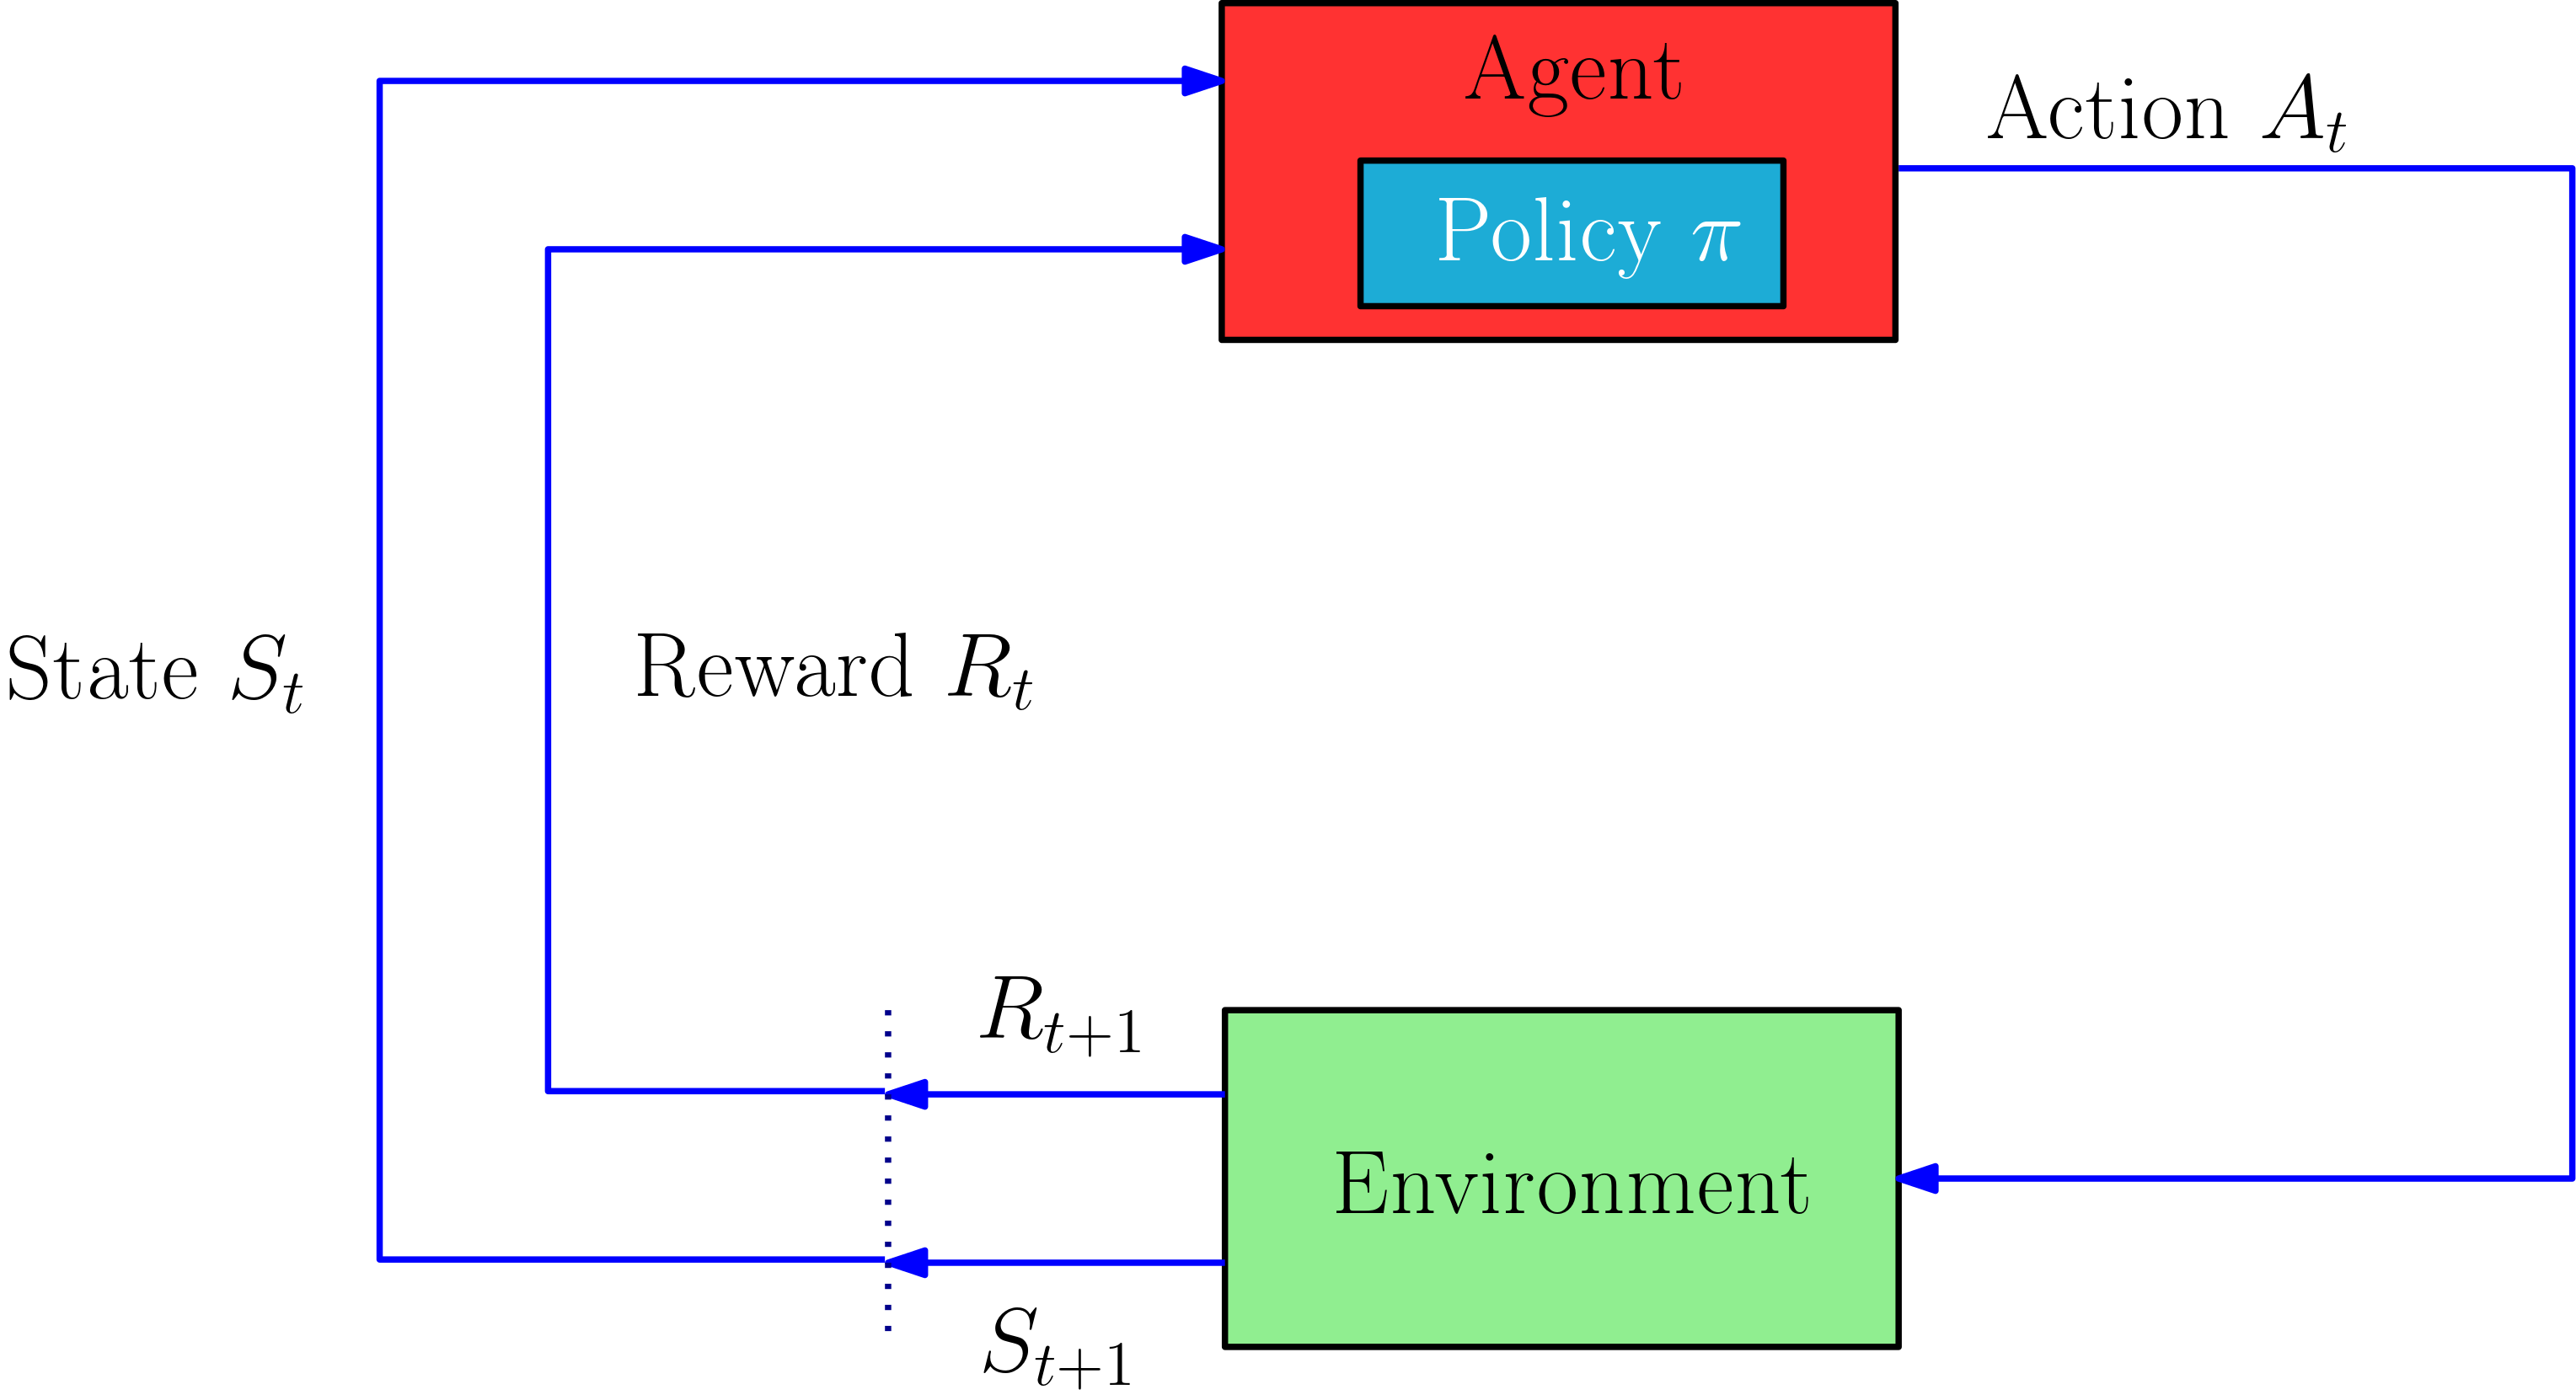
\includegraphics[width=0.9\textwidth]{images/rlv3.png}
    \caption{Reinforcement Learning}
    \label{fig:rl}
\end{figure}

% \begin{figure}[hbt] 
% \begin{center}
% \includegraphics[scale=.40]{./figures/bddig1}
% \caption{\label{fig:BDDD}A BDD where some boolean variables occur more than
% once on an evaluation path.}
% \end{center}
% \end{figure}

\subsection{DEEP REINFORCEMENT LEARNING}

We have already seen that in reinforcement learning, the agent tries to learn a policy $\pi$ in order to maximize its rewards. The policy $\pi$ is usually given by $\pi(s\gets a)$, a function mapping states to actions. In deep reinforcement learning we use neural networks to approximate the policy $\pi$, and other learnable functions such as the value function.

\begin{figure}[H]
    \centering
    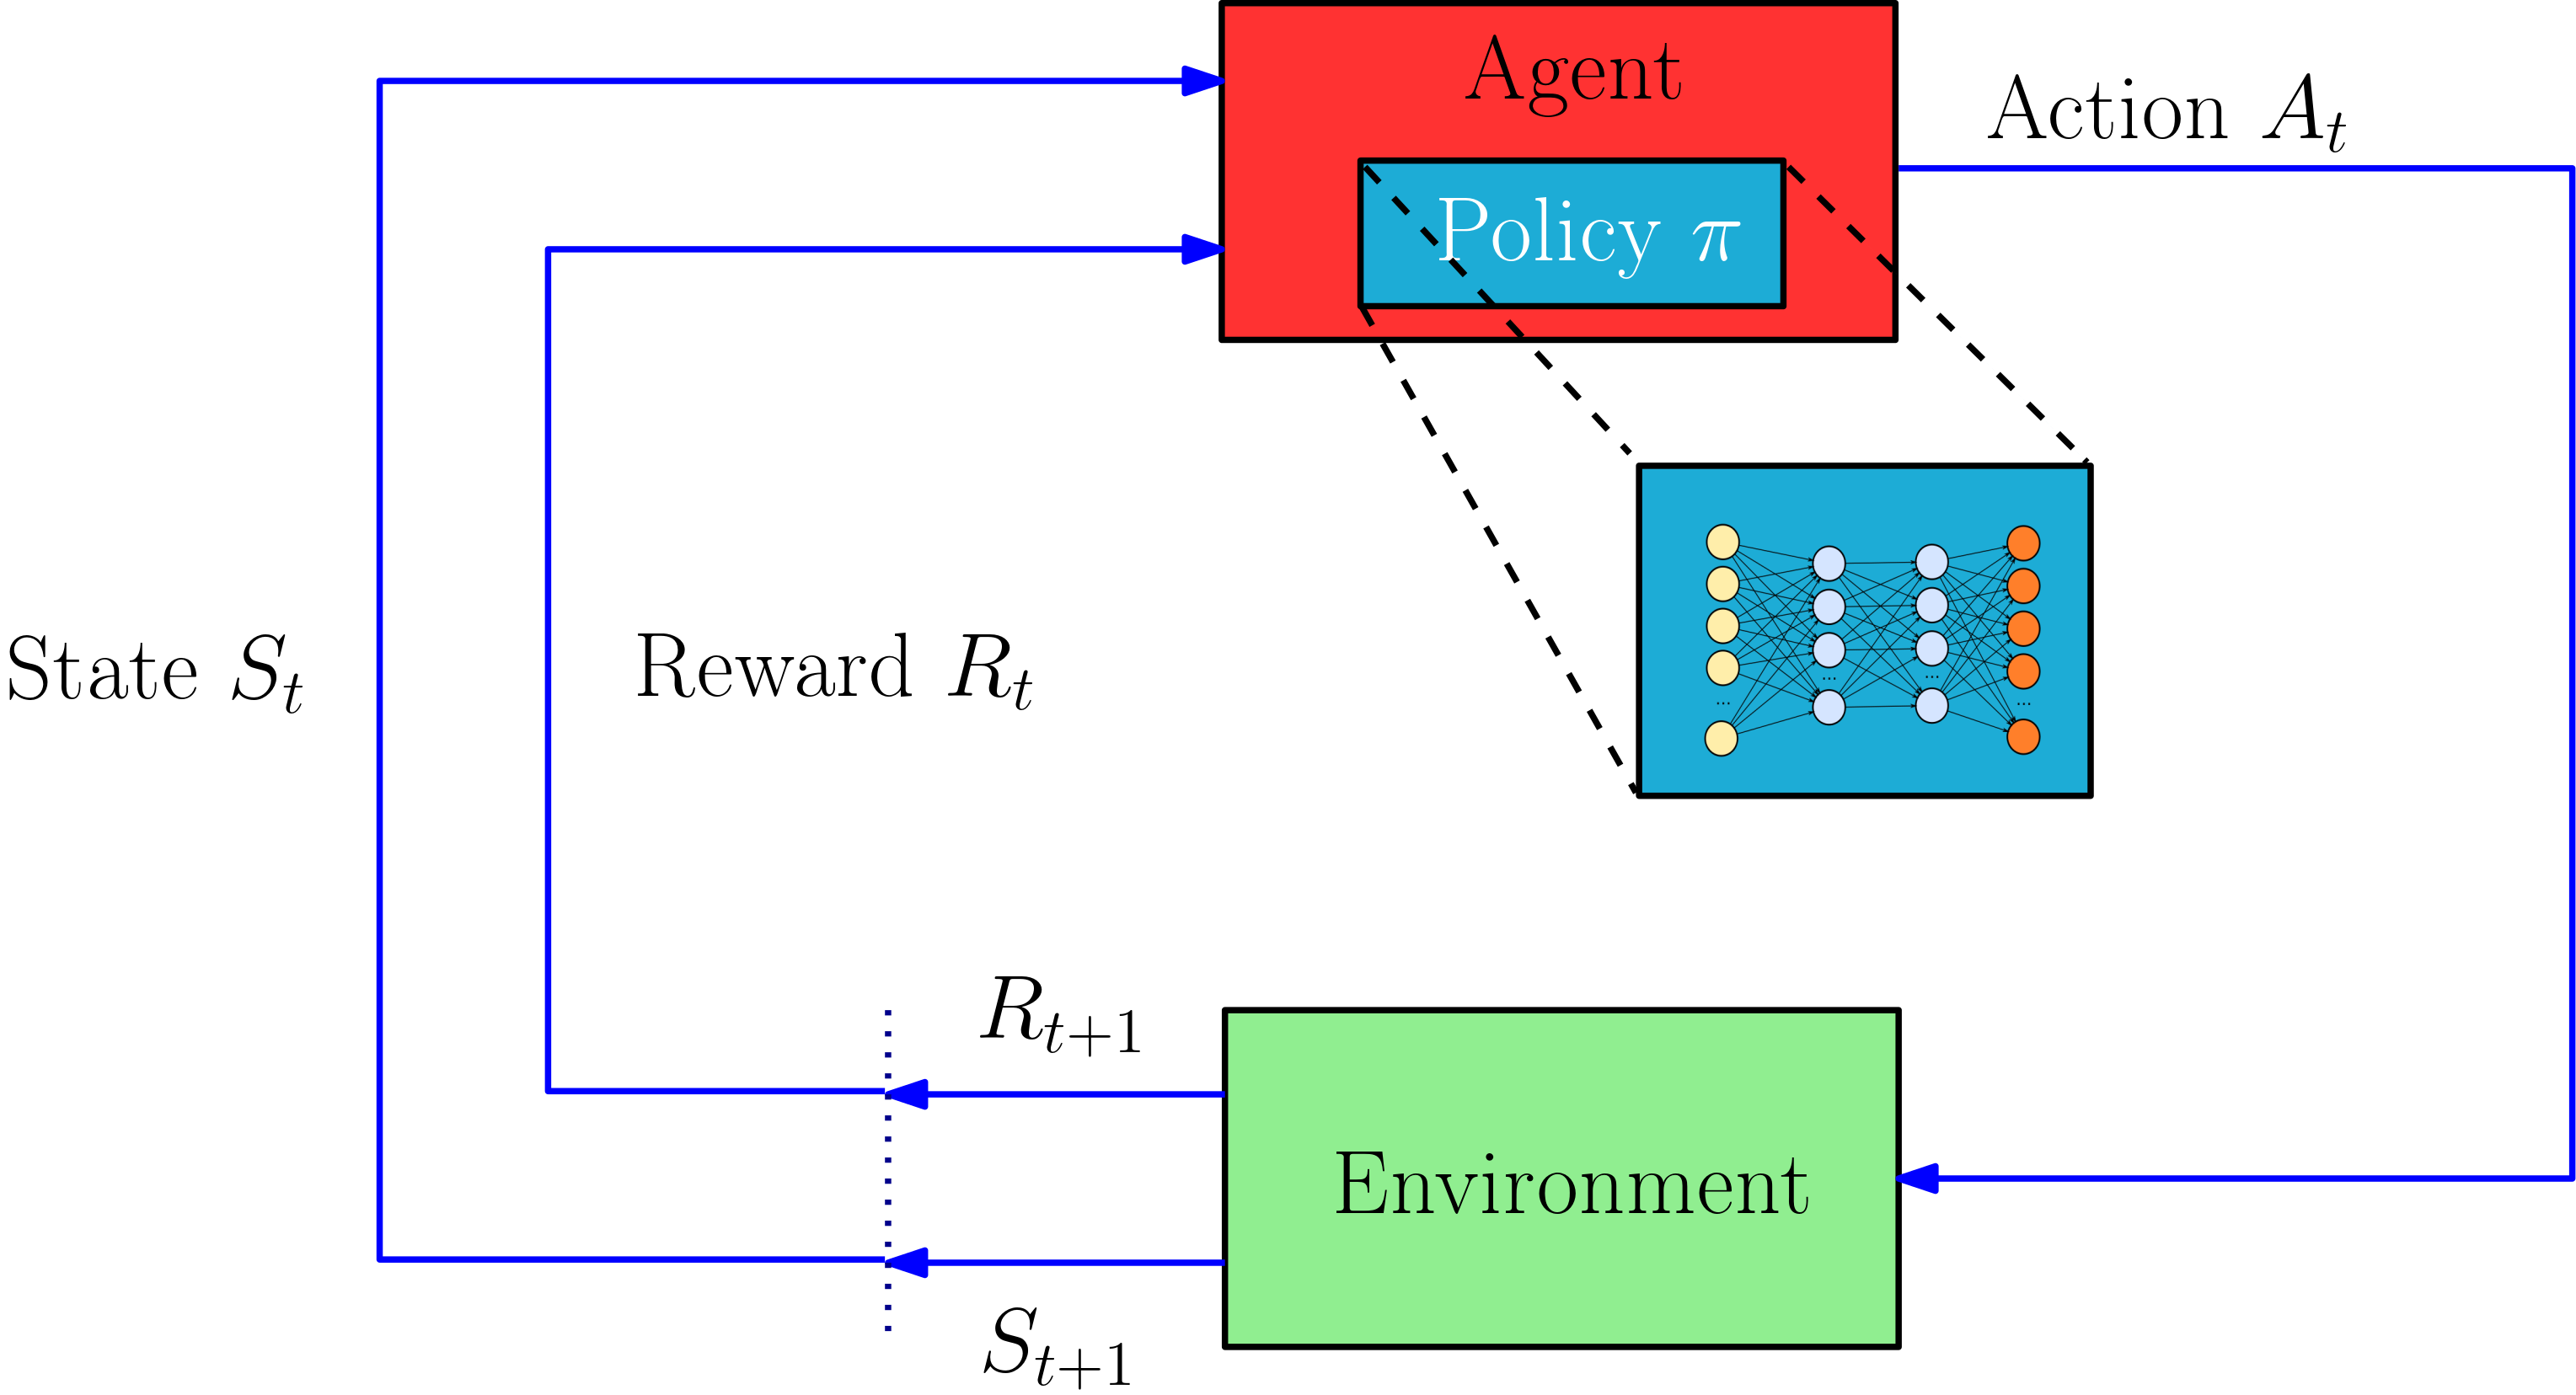
\includegraphics[width=0.9\textwidth]{images/drlv3.png}
    \caption{Deep Reinforcement Learning}
    \label{fig:rl}
\end{figure}

\section{TRANSFER LEARNING}


Transfer learning is a method that improves the performance on the target task by leveraging the knowledge gained by performing the same experiment on a similar source task. This can be often seen in supervised learning problems such as image labeling, where the knowledge from the source task is used to enhance the performance and efficiency of learning in the target task. However, this can be quite challenging in reinforcement learning, as each problem may have a different state space. We are able to utilize transfer learning to learn tasks that are rather similar, i.e, having a similar observation space and states.

\begin{figure}[H]
    \centering
    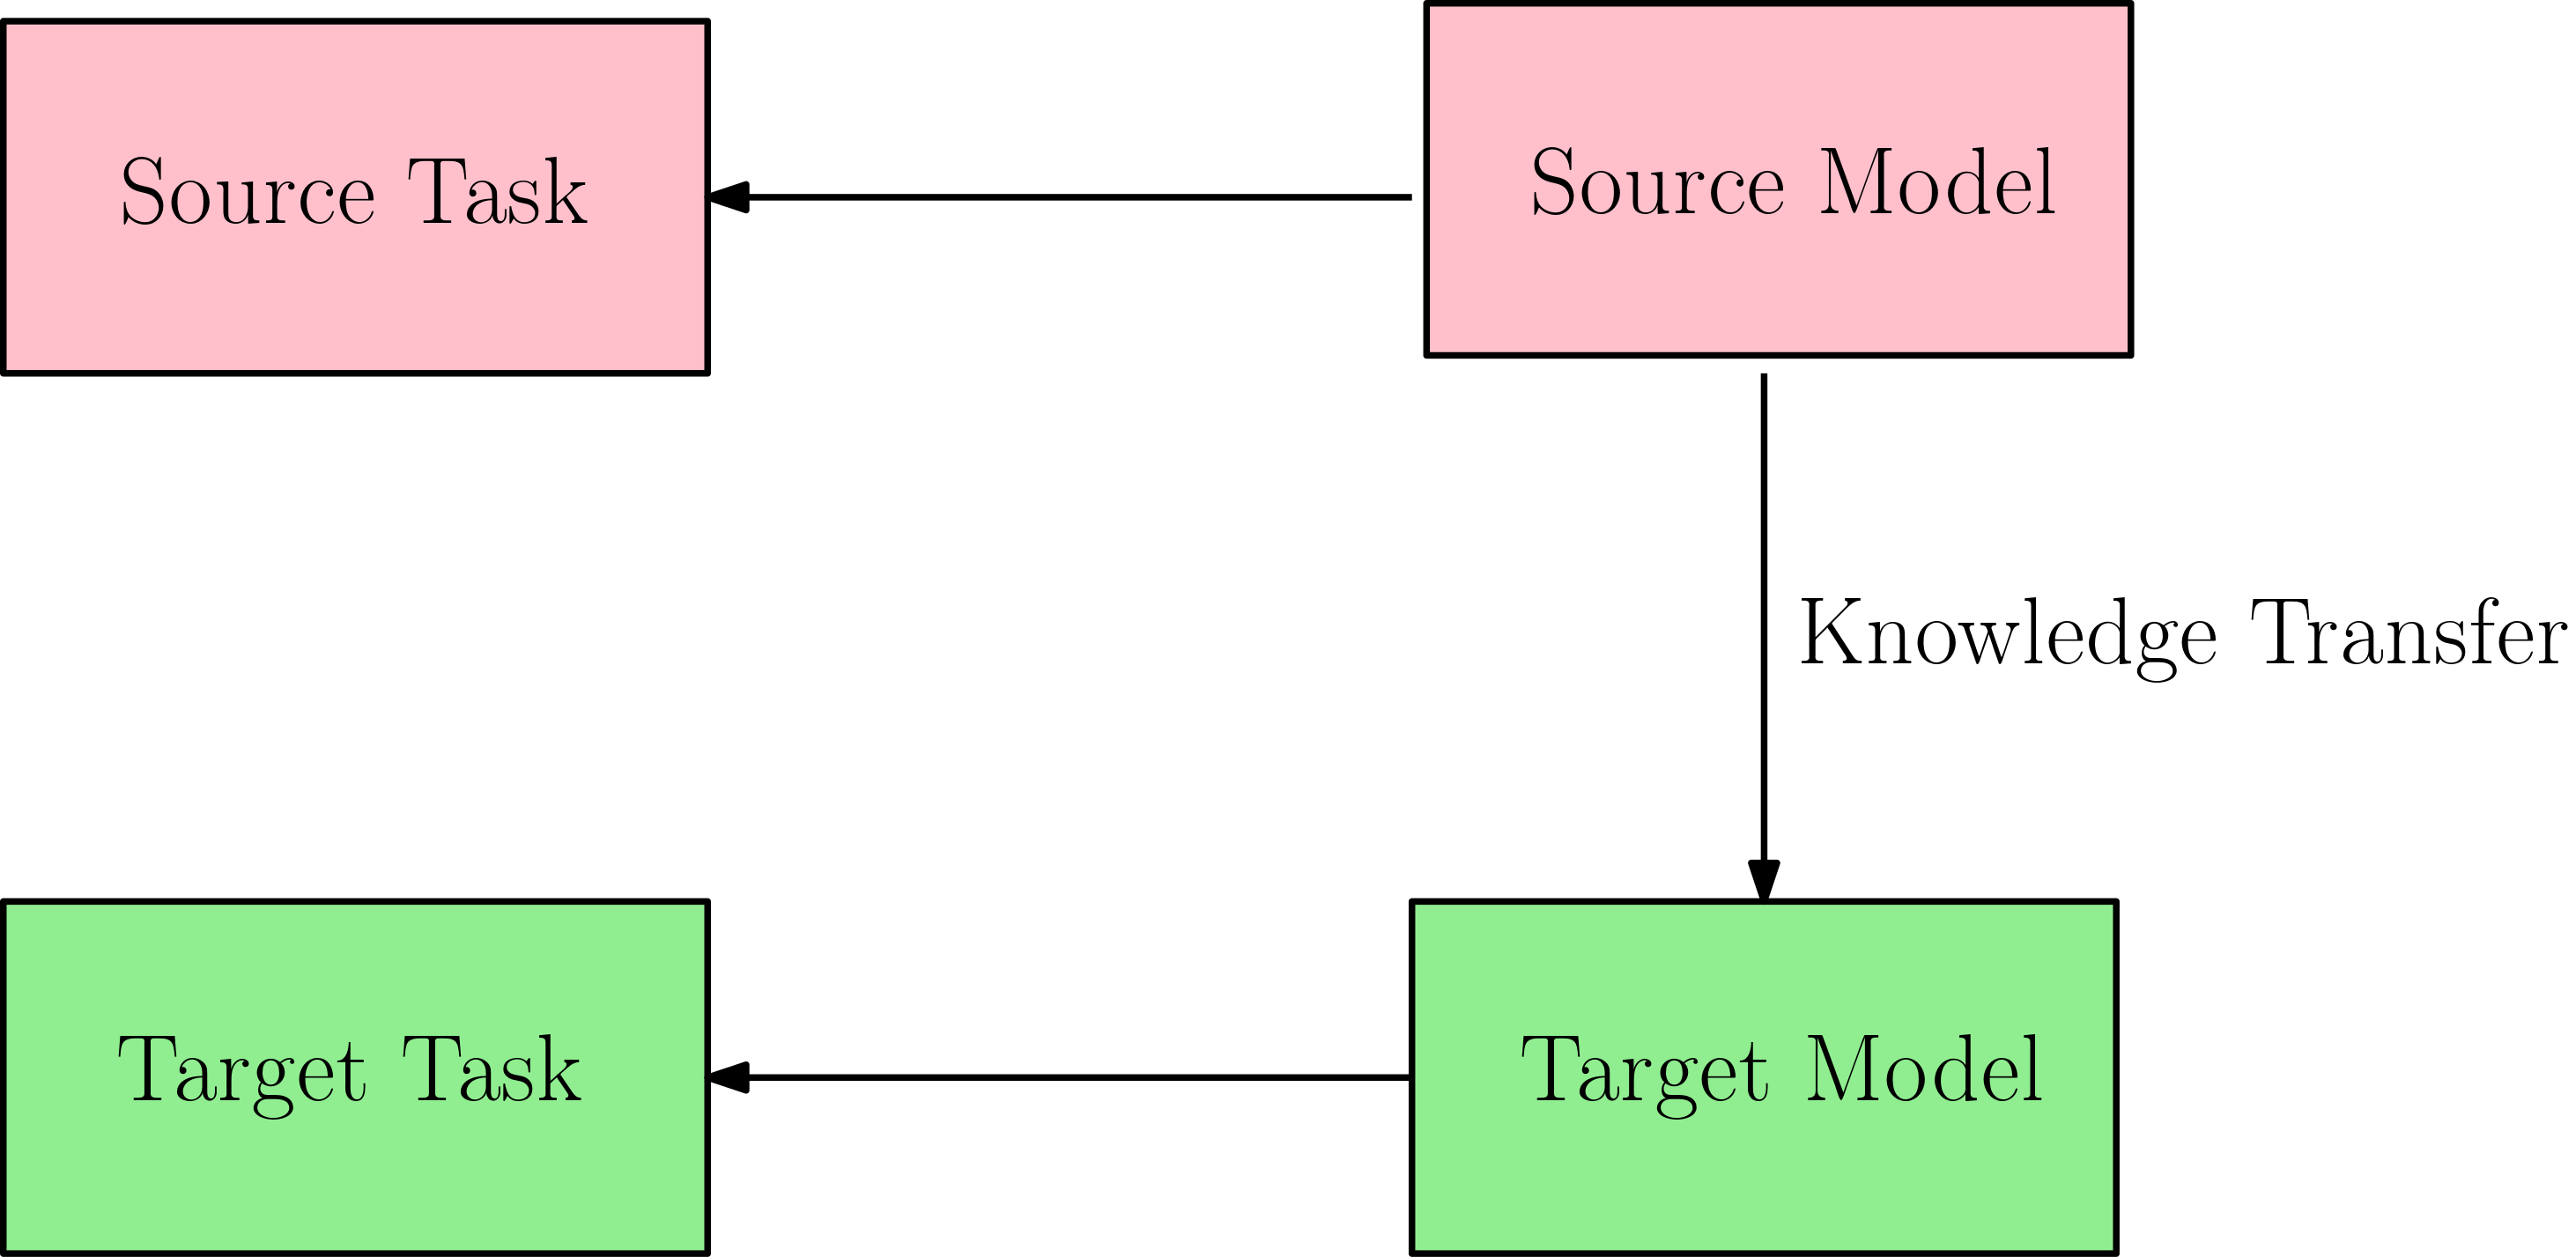
\includegraphics[width=0.9\textwidth]{images/tlv3.png}
    \caption{Transfer Learning}
    \label{fig:rl}
\end{figure}

\section{ADVERSARIAL TRAINING}

Many machine learning and deep learning models are often trained and tested on data from the same statistical distribution, and are hence often overtuned to perform well only on said distribution. This however causes issues when deployed with real world data and may be prone to adversaries that may take advantage of this fact and compromise the result of the model. Thus we use adversarial training to mitigate this concern. 

Adversarial training in reinforcement learning is made possible by using an adversary to attack the observations or the actions of the model. Knowing that adversarial training improves representational learning in supervised models, we can intuitively say that using adversarial training along with transfer learning will improve the performance of an agent using reinforcement learning.

\begin{figure}[H]
    \centering
    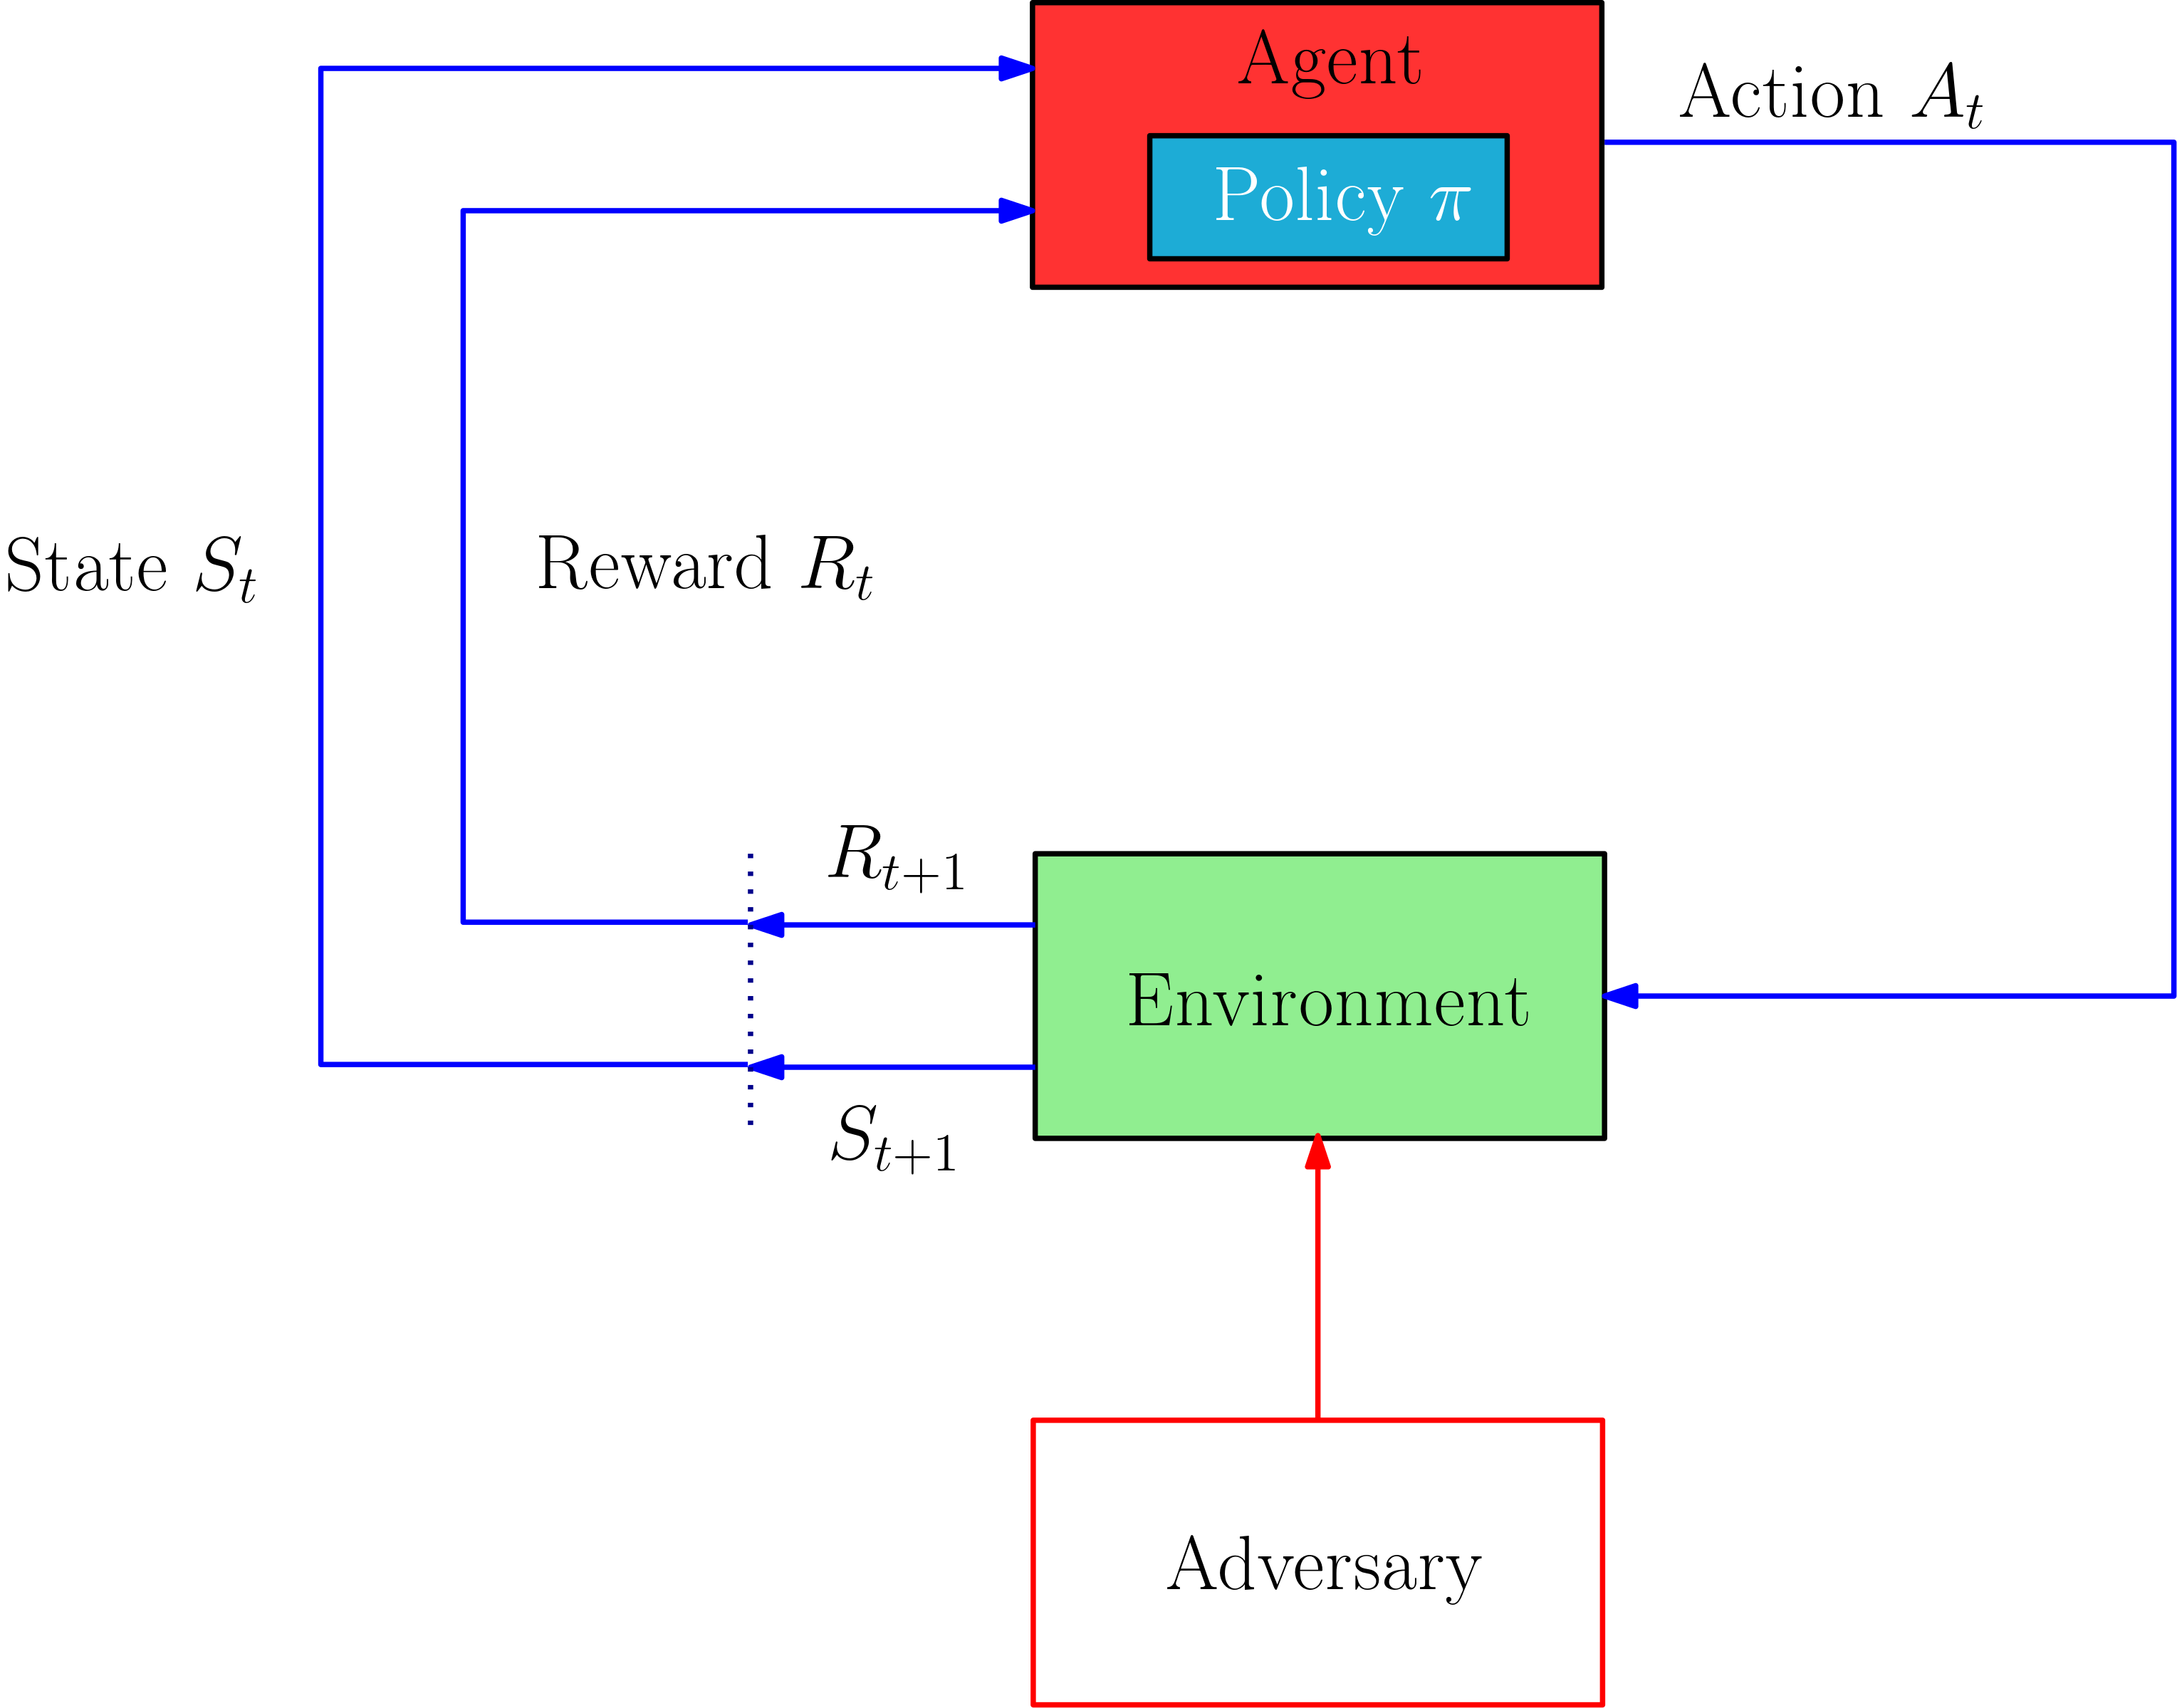
\includegraphics[width=0.9\textwidth]{images/rl_atv3.png}
    \caption{Adversarial Training in Reinforcement Learning}
    \label{fig:rl}
\end{figure}

\section{UNITY}

Unity is the game engine we used to create our environments. Unity allows us to create a 3D environment on which we can run our reinforcement learning algorithms. It uses a scripting API written in C\#. The engine also supports Object Oriented Programming paradigm, to create various game objects components that enable us to create an interactive environment for our agent.

Unity provides the user with a console, in which we can visualize the various components of the environments. The properties and functionalities of said components are defined in their respective script files. This gives us great control over the environment. We can set the goal state of the agent and define the various events on which we give the agent a reward, this is done by calling the API provided by unity. This flexibility in defining the problem makes Unity all the more alluring and our primary choice for creating an environment.

Unity provides a package known as MLagents, which provides a wrapper API and some baseline implementations of well known Deep Reinforcement learning algorithms. It also acts as the connector between the model and the environment enabling us to configure different models and train them in our environment.

 % LITERATURE SURVEY
% Chapter 2

\chapter{LITERATURE SURVEY} % Write in your own chapter title

This chapter covers the literature pertaining to Reinforcment Learning
(\ref{lit-rl}), Deep Reinforcement Learning (\ref{lit-drl}), Transfer
Learning (\ref{lit-tl}), Adversarial Training (\ref{lit-at}) and Unity
ML Agents (\ref{lit-mlagents}).

\section{REINFORCEMENT LEARNING} \label{lit-rl}

Reinforcement Learning refers to a trial-and-error interaction based
approach by which an agent learns to behave in its environment. This
is inspired by animal psychology study and has its roots in
statistics, psychology and computer science \cite{RLIntro}. Some early
real world applications of RL involved the usage of computer
simulation enhanced common sense based rules to create a fuzzy logic
system to design nuclear power plant control systems
\cite{RLNuke}. The usage of multi-layer perceptron as a function
approximator was first studied by \cite{RLMLP} for the cart pole
problem \cite{RLCartPole}.

\section{DEEP REINFORCEMENT LEARNING} \label{lit-drl}

Deep Reinforcement learning (DRL) has been able to solve a wide range
of complex decision-making tasks that were previously out of reach for
a machine \cite{DRL2}. Q-learning \cite{Qlearn} is a primitive RL
algorithm wherein the the value of the state is updated by performing
actions at the state and observing the rewards. Variations of
Q-learning allow us to successfully learn control policies directly
from high-dimensional sensory input using reinforcement learning
\cite{DRL1}. Actor critic DRL algorithims such as DDPG
\cite{cont-ddpg} and PPO \cite{ppo} can be used effectively in
continuous state space environments.

\section{TRANSFER LEARNING} \label{lit-tl}
%
Transfer learning is inspired by humans applying knowledge learned
previously to solve new tasks in a shorter amount of time and in an
improved manner in comparison to approaching the same task from
scratch \cite{TLInsp}. In the computer science domain, Transfer
Learning is the process of using knowledge learnt in source domains in
order to augment training and model performance in a similar target
domain \cite{transfer-rl}.

TL in Deep Learning(DL) has been successfully applied to obtain state
of the art performance on a smaller target dataset by transferring the
knowledge from a large source dataset \cite{TLDLBasic}. TL in DL has
been found to be resilient to the extent that even if the source
domains and target domains are quite distant, the performance obtained
by TL models outperforms the approach which uses random weight
initialization \cite{TLDLPower}.

TL in RL is more rigid in contrast to the DL equivalents; in RL based
algorithms, the agent's representaion of the world (its sensors and
actuators) need to remain the same with flexibility in the state and
action space of the agent. In cases where the semantics of the actions
vary across tasks, there is a requirement for a mapping function
between the two target tasks \cite{TLRLImplement}. Approaches for
transfer learning in RL are of five categories, namely, Reward
Shaping, Learning from Demonstrations, Policy Transfer, Inter-task
Mapping, and Representational Transfer \cite{tl-rl-survey}. Recent
research has shown that performance of TL models can be improved by
decoupling the processes of learning the domain and the reward
function \cite{tl-decoupling}.

\section{ADVERSARIAL ATTACK \& TRAINING} \label{lit-at}
%
Adversarial attacks were first investigated in \cite{ad-intro} wherein
the impact of adding noise to image data to misclassify the images was
studied. Initial methods to make models resilient to these attacks by
adding Gaussian Blur and AutoEncoders to negate some impact of
adversarial noise was studied by \cite{adreco1}. Other methods for
Adversarial defence were studied by performing image transformations
\cite{adreco2}.

Adversarial Training \cite{AT-Ian} also serves as a good form for
defence and is resilient against multiple forms of
attacks. Reinforcement Learning models, like Deep Neural Networks, are
impacted by adversarial attacks \cite{rlad1}. The RL agents can be
manipulated by using Fast Gradient Sign Method(FGSM) \cite{rl-fgsm} to
perturb observation frames in a Deep Reinforcement Learning setting or
dealing with an optimal adversarial agent, trained to drive the system
into suboptimal states \cite{rlad2}. Defending RL models from
Adversarial Attacks is best done by Adversarial Training methods like
\cite{rlat1} which makes use of Stochastic Gradient Langevin
Dynamics(SGLD).

\section{UNITY ML AGENTS} \label{lit-mlagents}

The ML agents toolkit is an open source package in Unity that provides
an intuitive and efficient way to create environments in Unity game
engine. The ML agents toolkit in Unity is used to create 2D and 3D
environments that enable reinforcement learning. Previous work with
the ML agents toolkit involves creating a single lane track for object
avoidance\cite{MLagents1}, and training actor critic algorithms on a
third person shooter gaming environment\cite{MLagents2}.





 % DESIGN
% Chapter 4

\chapter{SYSTEM ARCHITECTURE} \label{ch4}
This chapter describes the overall architecture of the project. The first section(\ref{ch4Env}) covers the custom environment that we have developed using Unity game Engine for conducting our experiment. We then describe our the agent(\ref{ch4Agent}) wherein the agent, the methods by which the agent perceives the environment (\ref{ch4inp}), obtains the rewards and takes decisions using the PPO algorithm are discussed . The penultimate section(\ref{ch4TL}) introduces the Transfer Learning process by which the knowledge learnt by the agent in one track is transferred to another track in our environment. Finally, we cover adversarial attacks(\ref{ch4AT}) on the action space and the observation space of the agent and performing Transfer Learning using Adversarial Training as a precursor.

\section{ENVIRONMENT} \label{ch4Env}



To perform Deep Reinforcement learning we have designed and created our own custom environment in Unity game engine. We have used a package called MLagents developed specifically for Unity that allows us to run our reinforcement learning algorithms in the environment.

We have designed 5 tracks of varying complexity to measure model performance in environments having the same action space. We shall further explore the different tracks in the upcoming chapters. 

Building the environment from scratch, allows us to have greater control over the different events that may occur and influence the agent. All the environments have similar events that are used to return a scalar reward to the agent.



The tracks are built using 4 major components : the sidewall(3), the checkpoints(2), the agent(1) and the ray perception sensors(4) as seen in figure \ref{fig:agent-inputs}

There are numerous checkpoints along the tracks that are placed approximately equidistant to one another. These checkpoints are used to encourage the agent to go in the right direction, and to measure how far the agent has progressed in a track. These invisible checkpoints have an event associated with them that enables the agent to detect them when a collision occurs. When this event is fired, we check if the current checkpoint is the correct checkpoint or not and appropriately provide a reward.

The sidewalls are solid game objects that are used to make sure the agent/car doesn't veer off track. When the agent collides with the sidewall, a function is triggered and a negative reward is sent to the agent. The ray-perception sensors are sensory beams originating from the car/agent, that allow the agent to detect the other game objects and components in the environment. The interactions between these 4 core components enable us to set our scalar rewards, that guide the agent and provide the essential logic required for training.


\subsection{REWARD SCHEME}

The reward scheme is crucial to enable the agent to train for the task. Rewards need to be provided at a constant interval when the agent is performing as expected in order to train faster and similarly negative rewards need to be provided immediately when performance is unexpected in order to train the agent faster. By experimenting with various permutations, we have arrived at the following reward scheme for the agent:

\begin{enumerate}
    \item \textbf{At each step}: A \textit{small negative} reward is provided to incentivize the agent to travel quicker around the track.
    \item \textbf{OnWallCollision:} A \textit{moderate negative} reward is provided to discourage agent from hitting the walls on the track.
    \item \textbf{OnWallCollisionStay:} The difference between collision stay and collision is that once an object has collided in Unity, if it is still in contact with the object post collision, a separate event called OnCollisionStay is triggered and hence a \textit{small negative} reward is provided to prohibit agent from using the walls to perform its turning actions.
    \item \textbf{CorrectCheckpoint:} The car has managed to make some progress in the track and hence to reward its progress, a \textit{positive} reward is provided.
    \item \textbf{IncorrectCheckpoint:} The car is moving in the wrong direction on the track and hence to prevent it from continuing to do so, we provide a \textit{negative} reward when it passes through an incorrect checkpoint.
    \item \textbf{LapCompleted:} The car has completed a lap successfully around the track and hence a \textit{large positive} reward is provided to the agent.
\end{enumerate}


\section{AGENT} \label{ch4Agent}

\subsection{Actor-Critic Methods}
Actor Critic Methods are a subclass of Reinforcement Learning algorithms. They consist of a “Critic” and an “Actor” entities during the training process. The “Critic” estimates the value function, ie, the value or predicted reward of a given state. This value function could be a state or action value function. The “Actor” in turn, makes use of the Critic’s output in order to update the policy distribution, and takes action based on the current policy. The samples generated by the Actor in turn, are used to update the value estimates of the Critic. Both the Actor and Critic are function approximators, generally with neural networks. 

\begin{figure}[H]
    \centering
    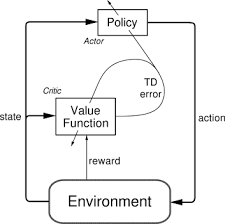
\includegraphics[width=0.45\textwidth]{images/ActorCriticMethod.png}
    \caption{Actor Critic Methods}
    \label{fig:rl}
\end{figure}

\subsection{Proximal Policy Optimization}
Proximal Policy Optimization (PPO) is an RL algorithm that falls under the actor-critic class of methods. It is a policy gradient method, ie, it uses a function approximator to represent the policy and performs gradient ascent on it to obtain the maximum reward. The main advantage of PPO over vanilla policy gradient or actor-critic algorithms is the fact that PPO clips the updates made to its value function to a certain extent. By clipping its updates, PPO ensures that the policy doesn’t go too far in the wrong direction and ruin its chances of finding the optimal solution.

In order to understand how PPO performs this clipping, we need to understand a few key terms first. The first term is $r(\theta)$. $r(\theta)$ is defined as the probability ratio of an action under the current policy and the action under the previous policy. If a particular action becomes more likely to be taken by the current policy, the value of $r(\theta)$ will be greater than 1. If a particular action becomes less likely to be taken by the current policy, the value of $r(\theta)$ will be between 0 and 1.

% \begin{figure}[H]
%     \centering
%     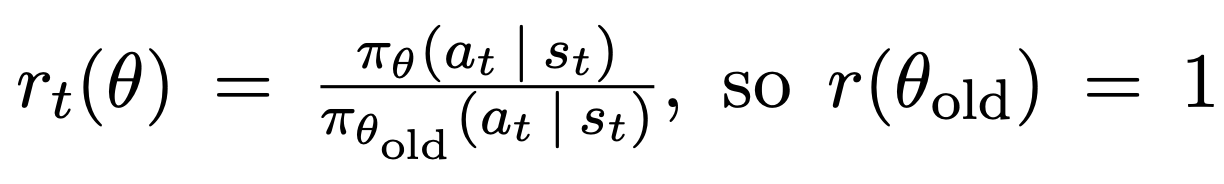
\includegraphics[width=0.75\textwidth]{images/r-theta.png}
%     \caption{r(theta)}
%     \label{fig:rl}
% \end{figure}


\begin{equation}
    r_{t}(\theta) = \frac{\pi_{\theta}(a_{t}|s_{t})}{\pi_{\theta}_{old}(a_{t}|s_{t})}, so\; r(\theta_{old}) = 1
\end{equation}


The second term is the advantage $\hat{A}_{t}$. The advantage $\hat{A}_{t}$ is an estimate of the relative value of the selected action in the current state. This advantage is used to estimate how good a particular action is compared to the average action in that state. The advantage is used to reduce variance in the updates made to the value function. If the advantage function for an action is positive, it means that action is good and will generate better rewards in the future. Therefore, we should increase the probability of picking that particular action in the future. On the other hand, if the advantage function for an action is negative, the probability of picking that action should be reduced.

% \begin{figure}[H]
%     \centering
%     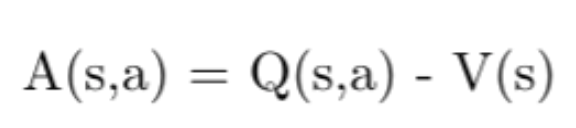
\includegraphics[width=0.75\textwidth]{images/advantage-function.png}
%     \caption{Advantage Function}
%     \label{fig:rl}
% \end{figure}
\begin{equation}
    A(s,a) = Q(s,a) - V(s)
\end{equation}
The general method in which policy-gradient methods work is by optimizing a policy loss function. Optimizing this function for reward can theoretically lead to an optimized function, but it is often quite difficult due to the nature of the samples. During the training process, the neural network representing our value function is constantly being updated, therefore our values are quite noisy and may not be very accurate.

PPO aims to solve this issue by making use of both of these terms, ie, $r(\theta)$ and $\hat{A}_{t}$, to generate a unique loss function called the Clipped Surrogate Objective. Clipped Surrogate Objective computes the minimum of two terms: the normal PG(Policy gradient) objective and clipped PG objective. The key component in PPO is the 2nd term, which clips the normal PG objective between $1 + \epsilon$ and $1 - \epsilon$. The effects of this clipping can be captured in the below graphs. 

% \begin{figure}[H]
%     \centering
%     
\includegraphics[width=0.75\textwidth]{images/clip-ppo.png}
%     \caption{Clipped Loss}
%     \label{fig:rl}
% \end{figure}

\begin{equation}
    L^{CLIP}(\theta) = \hat{\mathbb{E}}_{t}[min(r_{t}(\theta) \hat{A}_{t}, clip(r_{t}(\theta), 1- \epsilon, 1 + \epsilon)\hat{A}_{t})]
\end{equation}

\begin{figure}[H]
    \centering
    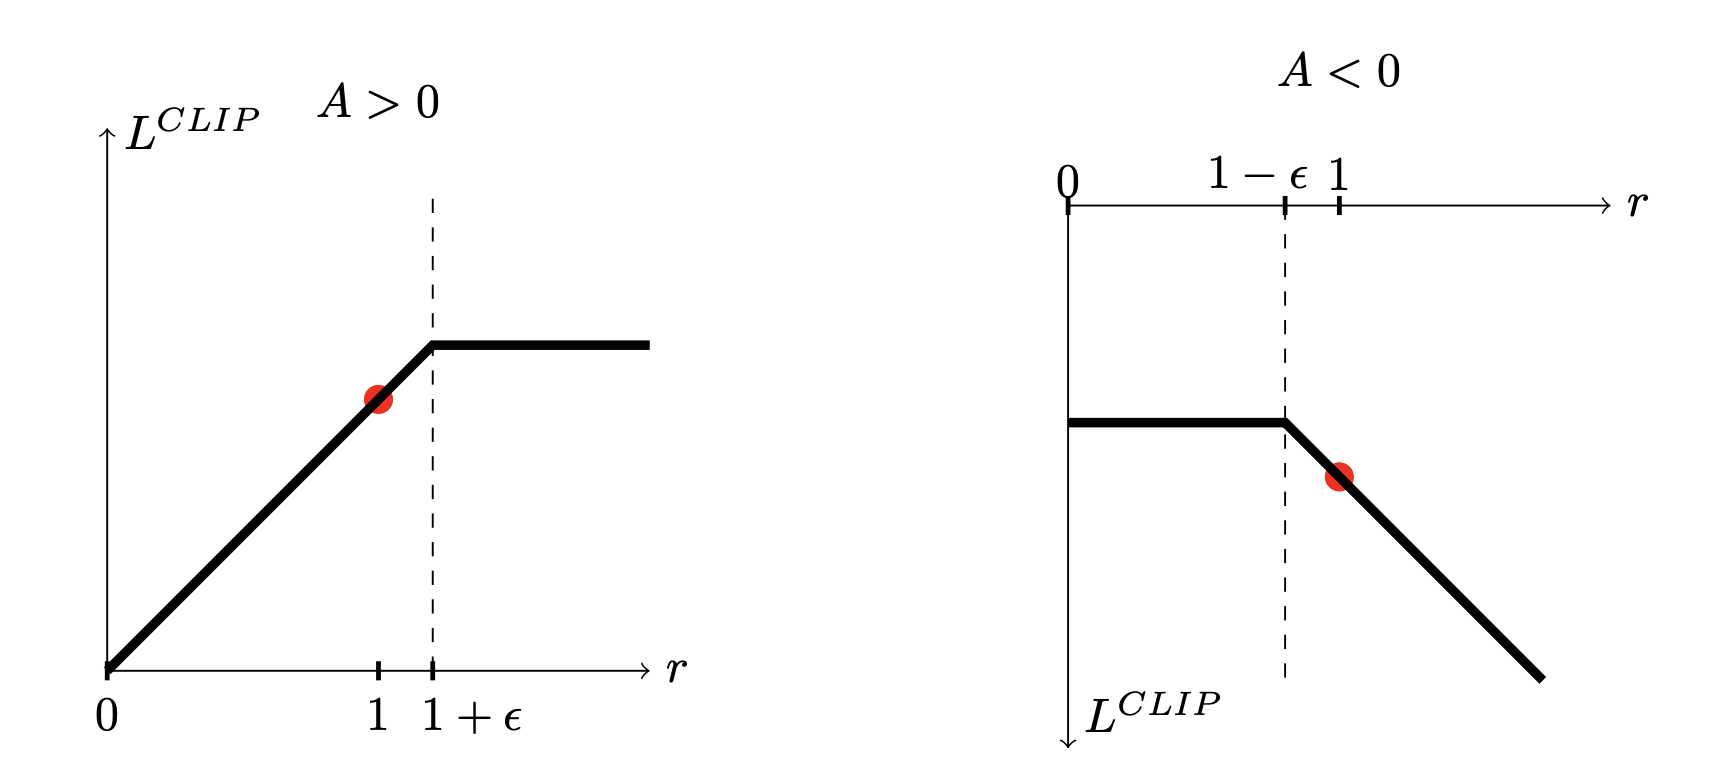
\includegraphics[width=0.75\textwidth]{images/clipped-loss-graph.png}
    \caption{Clipped Loss Graph}
    \label{fig:rl}
\end{figure}


On the left side, we see the scenario where the advantage is positive, i.e., the action taken by the agent had a better-than-expected return. With increasing values of r, the value of the $L^{CLIP}$ also increases, but only to a certain point. This prevents the algorithm from taking an update too far in the wrong direction. A similar scenario takes place on the right side as well. The algorithm is prevented from over-correcting its mistakes. 

PPO combines this loss function with two other terms, namely $L^{VF}$ and $S$. $L^{VF}$ is the mean squared error of the value function that is in charge of updating the network. S is a measure of entropy, which helps the agent act spontaneously in the initial stages of training, which can help the agent experiment and find optimal actions.



% \begin{figure}[H]
%     \centering
%     
\includegraphics[width=0.75\textwidth]{images/ppo-final-loss.png}
%     \caption{Final Loss}
%     \label{fig:rl}
% \end{figure}

\begin{equation}
    L_{t}^{CLIP+VF+S}(\theta) = \hat{\mathbb{E}}[L_{t}^{CLIP}(\theta) - c_{1}L_{t}^{VF}(\theta) + c_{2}S[\pi_{\theta}](s_{t})] 
\end{equation}

% \section{ALGORITHM: PPO} \label{ch4-ppo-alg}



\subsection{ALGORITHM: PPO} \label{ch4-ppo-alg}

% \begin{figure}[H]
%     \centering
%     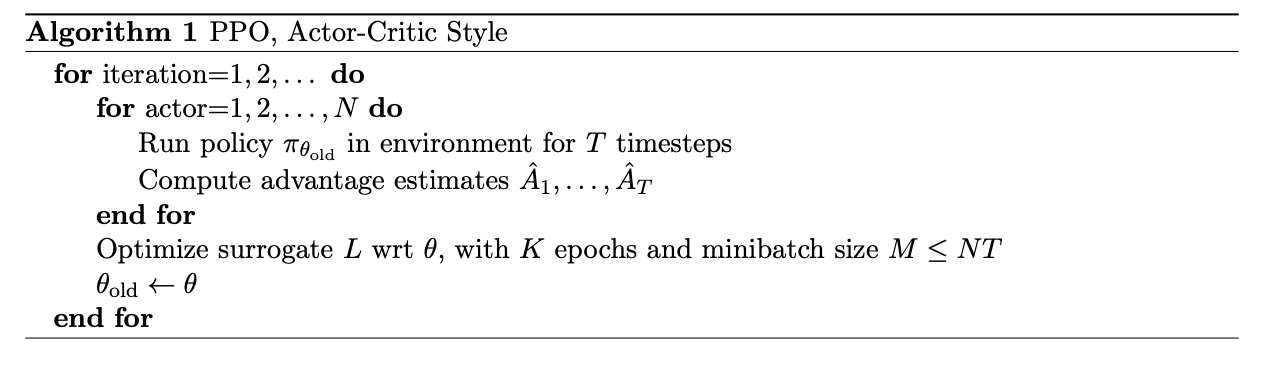
\includegraphics[width=0.95\textwidth]{images/ppo-algo.png}
%     \caption{Agent Inputs}
%     \label{fig:rl}
% \end{figure}


\begin{algorithm}[H]
\caption{Proximal Policy Optimization (PPO)}\label{alg:ppo}
\begin{algorithmic}
\For {iteration = 1,2,\ldots}
\For {actor = 1,2,\ldots,N}
\State Run policy ${\pi_{\theta}}_{old}$ in the environment for T timesteps
\State Compute advantage estimates $\hat{A_{1}}$,\ldots,$\hat{A_{T}}$
\EndFor
\State Optimize surroage $L$ wrt $\theta$, with K epochs and minibatch size $M \leq NT$\\
\State $\theta_{old} \gets \theta$
\EndFor
\end{algorithmic}
\end{algorithm}


\section{AGENT INPUTS} \label{ch4inp}

The agent in our environment is the Car(1) itself. The car makes decisions regarding acceleration deceleration and steering angle based on the inputs that it receives. The two major types of inputs that the agent perceives from the environment are the current speed and the Ray Perception Senor data(4) from the sensors placed on the car. The Ray Perception inputs inform the car of the distance of the object, what kind of object it is and also the angle from the car at which the object is located. For example, the object could be a Checkpoint(2) or a SideWall(3). The car makes use of this information to decide when to accelerate, brake, or turn.

\begin{figure}[H]
    \centering
    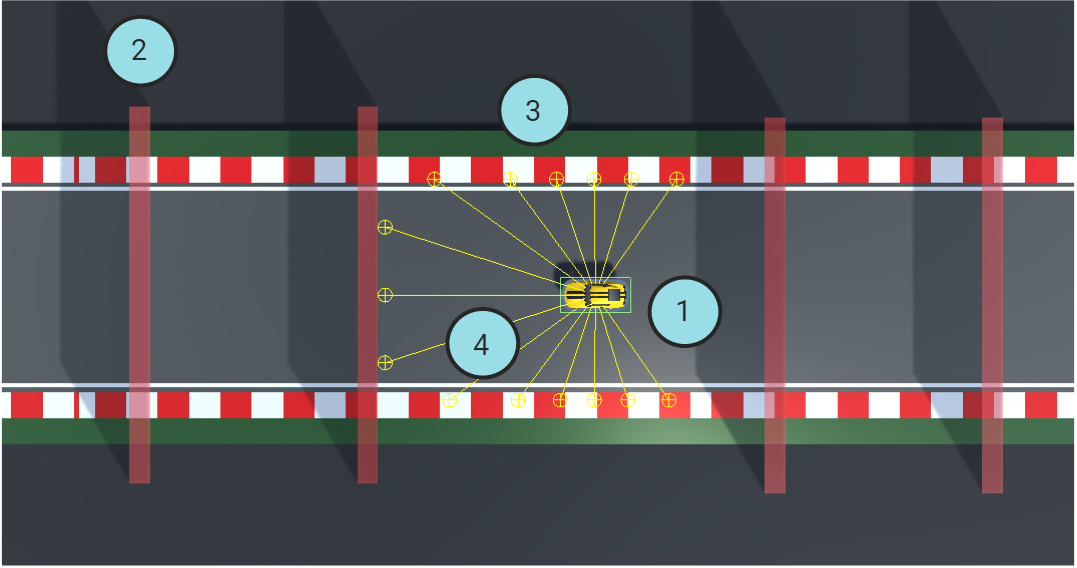
\includegraphics[width=0.75\textwidth]{images/UnityEnv.png}
    \caption{Agent Inputs}
    \label{fig:agent-inputs}
\end{figure}

\section{TRANSFER LEARNING} \label{ch4TL}
Upon training the models on the basic tracks developed using the PPO Algorithm, we then move on to creating complex tracks which we cover in section \ref{ch5} for the purposes of studying the results obtained by using Transfer Learning in our environment. 
\\ We study the performance obtained by TL when the similarity is high (intra basic track) and similarity is lower (basic track - complext track). It is to be noted that the latter is more dissimilar only when compared to the former and that in both cases the source task and the target task have the same task structure, satisfying the requirement to perform TL in RL \cite{TLRLImplement}. We peform these experiments to understand the difficulties associated with using TL in RL to leverage learned representation. 
\\To measure the performance of TL in RL in our environment, we measure the cumulative reward obtained at the end of fixed amount of steps on the target task and compare it with the cumulative reward obtained by training for the same number of steps on the target task with no prior knowledge. We also monitor the variance in  episode length as it is an indicator of the stability of the agent on the track.


\section{ADVERSARIAL  TRAINING} \label{ch4AT}
Finally, we perform Adversarial Attack and Adversarial Training in our environment using noise based attacks on the observations(\ref{at-obs}) and on the action space (\ref{at-action}).
\subsection{Attack on Observation} \label{at-obs}
The observations perceived by the agent are the current speed of the car and the distance and angle at which the checkpoints and walls of the track are located at. For the purposes of attacking the observation space, we add noise to the checkpoint positioning resulting in sub-optimal checkpoint orientation on track. Upon passing through a `attacked checkpoint', we attack the successive checkpoint and finally all checkpoints are reset at the time of lap completion.
\begin{algorithm}[H]
\caption{Adversarial Attack on Checkpoints}\label{alg:cap}
\begin{algorithmic}
\Require checkpointAtttackFlag = True
\State checkpointList[] $\gets$ track.getCheckpointList()
\State nextCheckpoint = 0
\While{lapCompleted = False}
\State $X_{disp} \gets$ Random.RandInt(-4, 4)
\State $Y_{disp} \gets$ Random.RandInt(-4, 4)
\State checkpointList[nextCheckpoint].position += ($X_{disp}$, $Y_{disp})$\\
\State nextCheckpoint = (nextCheckpoint + 1) \% totalCheckpoints\\
\If{nextCheckpoint = 0} \Comment{All checkpoints passed}
\State lapCompleted $\gets$ True
\State reset positions of all checkpoints
\EndIf
\EndWhile
\end{algorithmic}
\end{algorithm}

\subsection{Attack on Action Space} \label{at-action}
In this attack, we randomly pick actions ignoring the output provided by the policy of the agent during a fraction of time steps determined by a parameter called \textit{actionAdversaryThreshold}.

\begin{algorithm}[H]
\caption{Adversarial Attack on Actions}\label{alg:cap}
\begin{algorithmic}
\Require actionAdversaryThreshold $\geq$ 0, policy $\pi$
\State action $\gets \pi$.getAction() 
\State forward = action[0]
\State turn = action[1]
\If{Random.Rand() $\geq$ actionAdversaryThreshold} 
\State $forward \gets$ Random.RandInt(-1, 2)
\State $turn \gets$ Random.RandInt(-1, 2)
\EndIf
\State car.forward = forward
\State car.turn = turn
\end{algorithmic}
\end{algorithm}


We perform experiments and train agents on all the basic and complex tracks using both the attacks as  a precursor and repeat the experiments performed for TL in \ref{ch4TL} and study the performance of TL obtained using AT as a precursor and in the absence of AT.

 % IMPLEMENTATION
% Chapter 5 Experimental Setup

\chapter{EXPERIMENTAL SETUP} \label{ch5}
In this chapter we discuss the method used to measure the complexity of any given race track following which we move on to describe tracks developed for performing our experiments using the custom environment discussed in Chapter \ref{ch4}. We have developed 5 different types of tracks in two levels of complexity. The first level of complexity is called `Basic Tracks' . The second level of tracks are inspired by AWS Deepracer \cite{deepracer} challenge tracks and are inspired by real world race tracks with much higher level of complexity and are labelled `Complex Tracks'.


\section{TRACK COMPLEXITY MEASURE}
Before proceeding with the Basic and Complex Tracks, we will introduce the features used to quantify the complexity of a track. Features indicating the complexity of the track in decreasing order of complexity are as follows:
\begin{enumerate}
    \item Chicanes
    \item Sharp Turns
    \item Sweeping Turns
    \item Distance of Track
\end{enumerate}
\subsection{Chicanes}
Chicanes refer to a tight sequence of corners in alternate directions. They are usually inserted into a circuit to slow the cars, often just before a high-speed corner \cite{F1Chicane}. These are the most complex for the agent to navigate due to slow speed required and precise control of the turn inputs in order to pass the chicane without hitting the sidewalls of the track. The leeway for error is the least when navigating a chicane due to this nature. Figure \ref{fig:chicane} depicts an example of a chicane.
\begin{figure}[H]
    \centering
    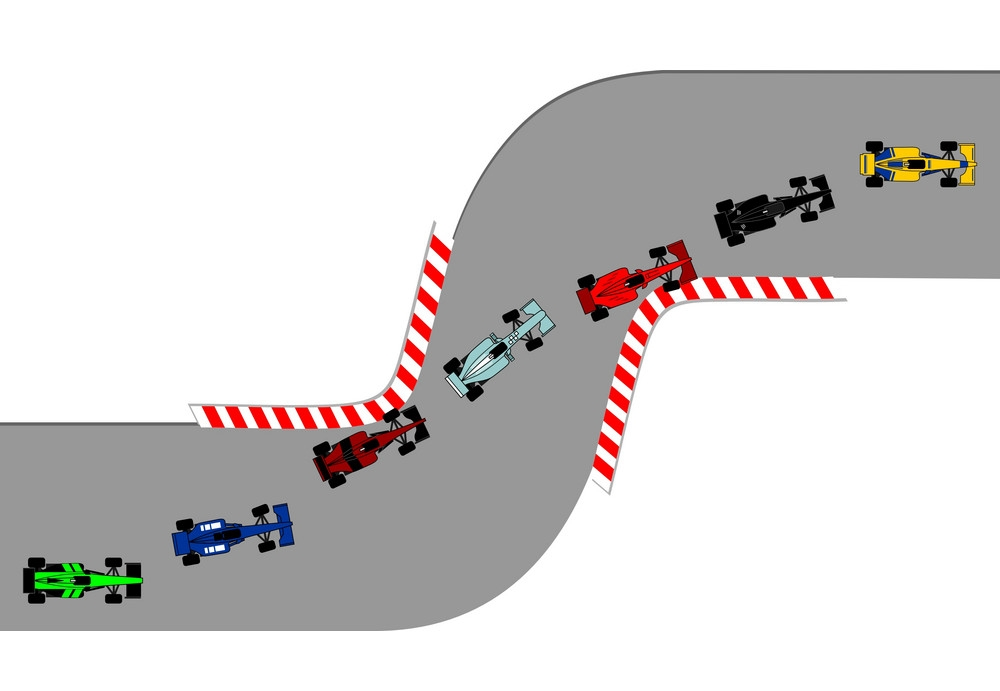
\includegraphics[width=0.7\textwidth]{images/Chicane.jpg}
    \caption{Chicane example (Image from \href{https://www.vectorstock.com/royalty-free-vector/chicane-road-circuit-vector-7128004}{Vector Stock})}
    \label{fig:chicane}
\end{figure}
\subsection{Sharp Turns \& Sweeping Turns}
The difference betwen Sharp Turns and Sweeping Turns is the radius of the turn. Turns with a lower radius are more difficult to navigate and the average speed of the car(agent) is lower and these are called sharp turns. Sweeping turns are turns having a larger radius of curvature allowing for faster speeds and minimal steering input allowing for more leeway for errors in the inputs. Figure \ref{fig:turns} shows the different types of turns.

\begin{figure}[H]
    \centering
    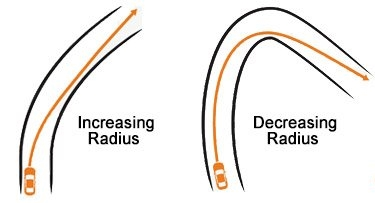
\includegraphics[width=0.5\textwidth]{images/Turn-Types-crop.jpg}
    \caption{Sweeping vs Sharp Turns (Image from \href{https://go-kart-source.com/go-kart-cornering/}{Go-Kart-Source})}
    \label{fig:turns}
\end{figure}

\subsection{Distance}
Distance of the track is the least important feature for track complexity. For the same given distance, the presence of more chicanes and/or turns determines the real world complexity in navigating the track. Thus, distance of the track is the least important feature to determine the complexity of a track. However, it is to noted that longer the distance, the chances for making a mistake increases due to the time taken to complete a lap around the track.

\subsection{Computing Complexity}
In order to quantify the complexity of a track, we use a custom metric given by
\begin{equation}
    Complexity = (4 \times Chicanes) + (2 \times SharpTurns) + SweepingTurns     
\end{equation}

% +  \frac{10 \times TotalTurns}{distance}

The complexity of all the tracks developed in our custom environment are provided in table \ref{tab:complexity}.
\section{BASIC TRACKS} \label{ch5-basictrack}
In this section we cover the basic tracks we developed as a part of Phase I of our experimentation. We developed the Oval track, shown in figure \ref{fig:ovaltrack}, which is the simplest of the tracks in terms of layout as a proof of concept tracks to ensure all our supporting systems like the checkpoint-ing systems were working as expected in our custom built environment. To test the the agent behaviour when more complicated maneuvers are required, we developed the One Kink Track and Two Kink track as shown in figures \ref{fig:onekink} \& \ref{fig:twokink}.

\begin{figure}[H]
    \centering
    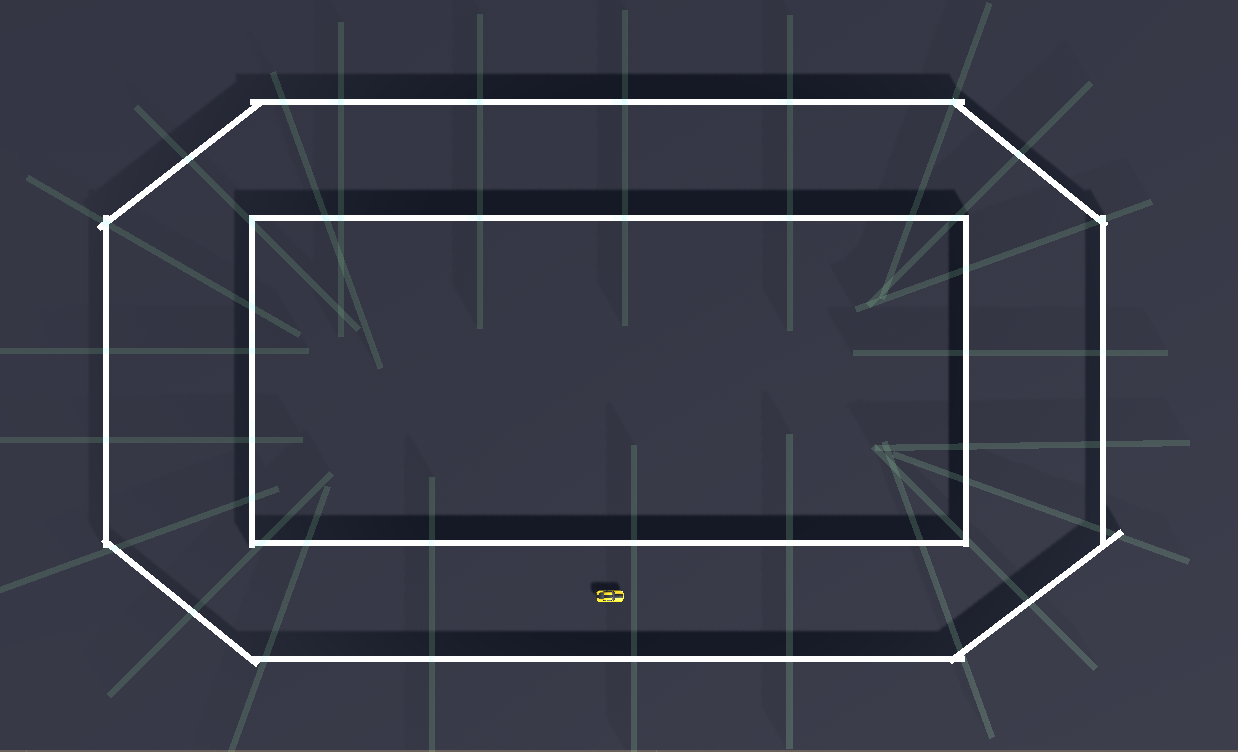
\includegraphics[width=0.90\textwidth]{images/tracks/OvalTrack.png}
    \caption{ Oval Track}
    \label{fig:ovaltrack}
\end{figure}
\begin{figure}[H]
    \centering
    \begin{minipage}[b]{0.45\textwidth}
    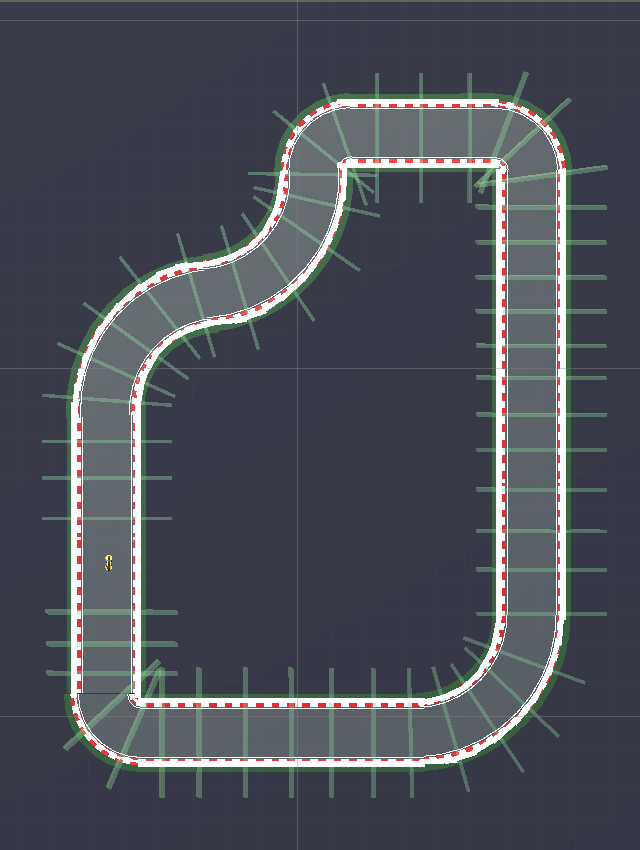
\includegraphics[width=\textwidth]{images/tracks/ComplicatedTrack.PNG}
    \caption{One Kink Track}
    \label{fig:onekink}
  \end{minipage}
  \hfill
  \begin{minipage}[b]{0.45\textwidth}
    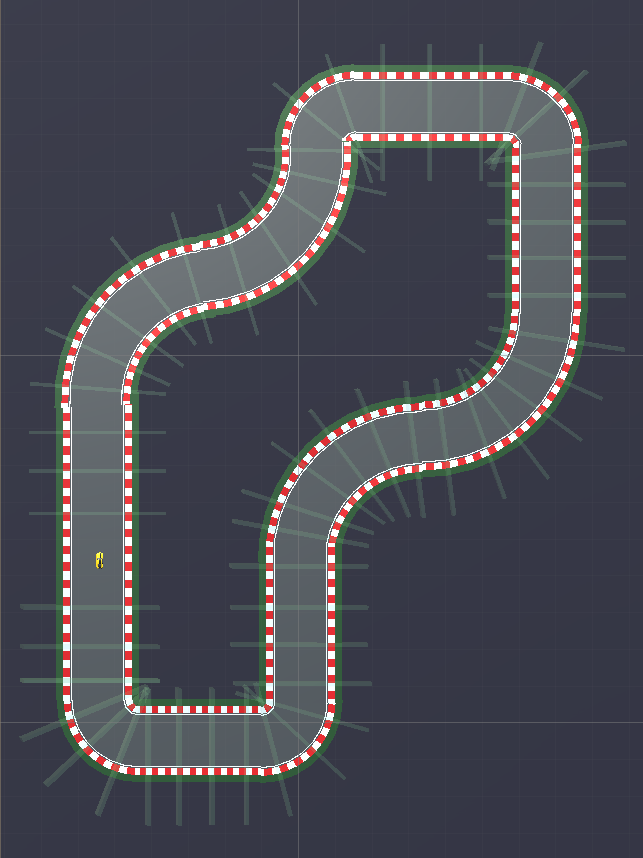
\includegraphics[width=\textwidth]{images/tracks/EvenMoreComplicatedTrack.PNG}
    \caption{Two Kink Track}
    \label{fig:twokink}
  \end{minipage}
  
\end{figure}
\section{COMPLEX TRACKS}
For developing `complex tracks', we have used a real world Formula 1 race track of barcelona and a track used as a part of AWS deepracer challenge namely AWS Asia Pacific Track to serve as inspirations to test the agent performance in tracks closer to real world. These tracks are longer and feature more complicated track layout in  comparison to the basic tracks discussed in section \ref{ch5-basictrack}.
\begin{figure}[H]
    \centering
    
\includegraphics[width=1.0\textwidth]{images/tracks/BarcelonaOG.png}
    \caption{Original Barcelona Racerack (Image from \href{https://www.clipartmax.com/download/m2H7G6d3Z5A0G6d3_circuit-de-barcelona-catalunya-el-circuit-restaurant-barcelona-f1-circuit-map/}{Clipartmax})}
    \label{fig:barcelona}
\end{figure}


\begin{figure}[H]
    \centering
    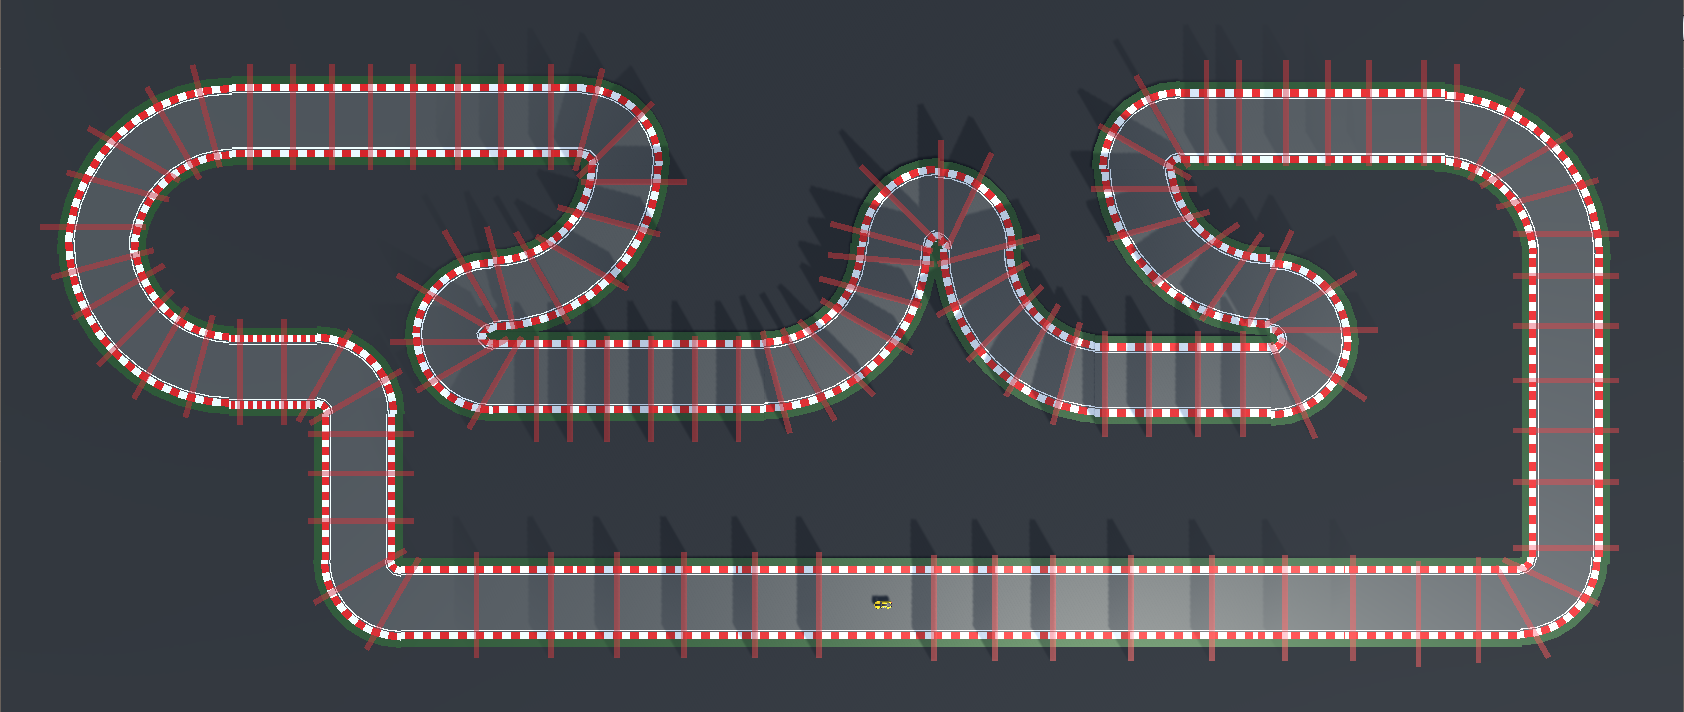
\includegraphics[width=1.0\textwidth]{images/tracks/Barcelona.png}
    \caption{Barcelona Track in Unity}
    \label{fig:barcelona}
\end{figure}

\begin{figure}[H]
    \centering
    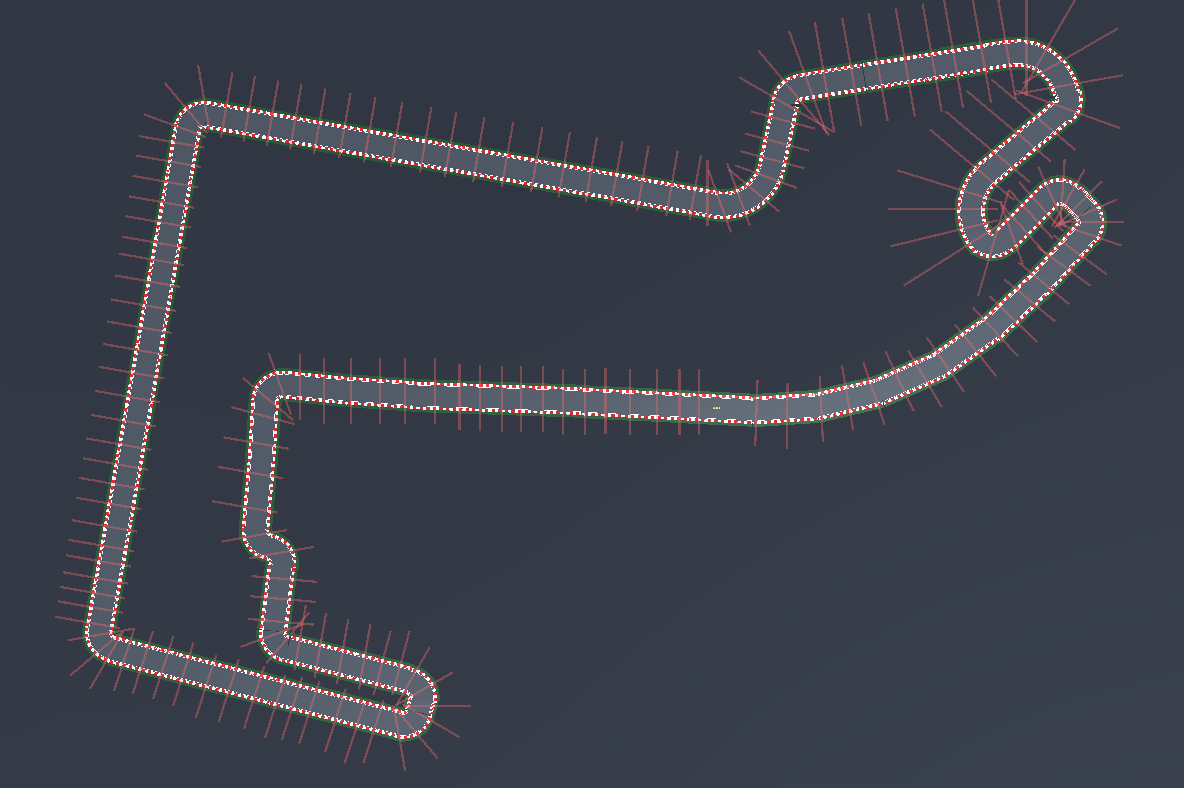
\includegraphics[width=0.9\textwidth]{images/tracks/AWSTrack.png}
    \caption{ AWS Asia Pacific Track}
    \label{fig:awstrack}
\end{figure}



\begin{table}[H]
\centering
\begin{tabular}{|p{1.9cm}|p{2.5cm}|p{2cm}|p{1.8cm}|p{2cm}|p{3.5cm}|}
\hline
\textbf{Type}                                         & \textbf{Track} & \textbf{Chicanes (C)} & \textbf{Sharp Turns (SH)} & \textbf{Sweeping Turns (SW)} & \textbf{Complexity \newline (4C+2SH+SW)} \\ \hline
\multicolumn{1}{|c|}{\multirow{3}{*}{\textbf{Basic}}} & Oval     & 0                     & 4                         & 0                            & 8                                      \\ \cline{2-6} 
\multicolumn{1}{|c|}{}                                & One Kink       & 1                     & 3                         & 1                            & 11                                     \\ \cline{2-6} 
\multicolumn{1}{|c|}{}                                & Two Kink       & 2                     & 4                         & 0                            & 16                                     \\ \hline
\multirow{2}{*}{\textbf{Complex}}                     & Barcelona      & 0                     & 8                         & 6                            & 22                                     \\ \cline{2-6} 
                                                      & AWS Track      & 1                     & 8                         & 4                            & 24                                     \\ \hline
\end{tabular}
\caption{Complexity of the various tracks developed}
\label{tab:complexity}
\end{table}

% \section{AGENT INPUTS}

% The agent in our environment is the Car(1) itself. The car makes decisions such as when to accelerate and when to brake based on the inputs that it receives. The two inputs that the agent receives are the current speed and the Ray Perception inputs(4) from the sensors placed on the car. The Ray Perception inputs inform the car of the distance of the object, and also what kind of object it is. For example, the object could be a Checkpoint(2) or a SideWall(3). The car can make use of this information to decide when to accelerate, brake, or turn.


\section{ML AGENTS}
MLagents is an open source package that provides a framework to train and develop intelligent agents in the Unity game engine environment. It supports multiple methods of training intelligent agents using reinforcement learning, imitation learning, and other machine learning methods through the Python API provided. ML Agent contains 4 major components as shown in image \ref{fig:mlagents}

\begin{figure}[H]
    \centering
    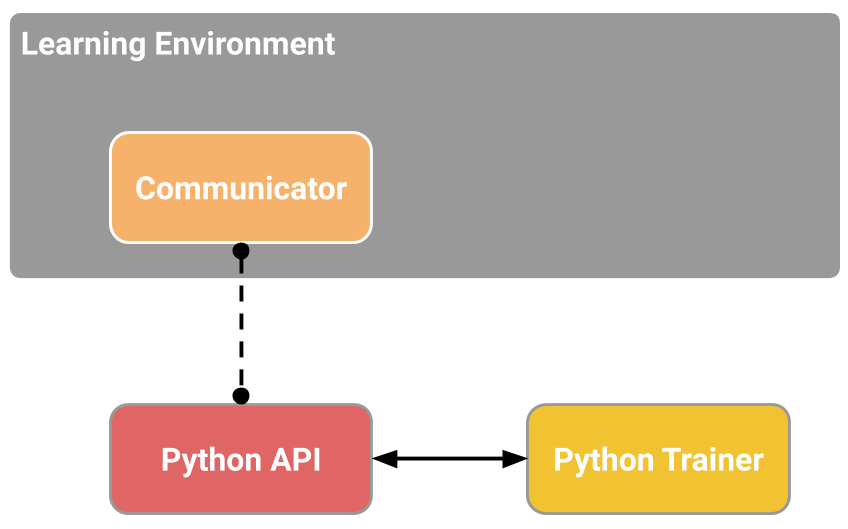
\includegraphics[width=1.0\textwidth]{images/mlagents.png}
    \caption{Components of ML Agents Framework (Image from \href{https://github.com/Unity-Technologies/ml-agents}{ML Agents Github})}
    \label{fig:mlagents}
\end{figure}

\begin{itemize}
    \item \textbf{Learning Environment:} Refers to the Unity scene created for experimentation. This scene serves as the environment for the agent to interact with and receive observations and take actions in.
    \item \textbf{External Communicator: } Feeds the data from the Unity scene and passes it on to the python API
    \item \textbf{Python API: } Provides for a method to directly access the Learning Environment from the external python code to interact and manipulate the learning environment
    \item \textbf{Python Trainer: } Is the place where the Algorithm used to train the agent is located. The algorithm has access only to the Python API and are written using PyTorch \cite{Pytorch}
\end{itemize}

\section{PPO NETWORK \& HYPER-PARAMETERS}

The algorithm we use to train our agents in the environment is the PPO Algorithm covered in section \ref{ch4-ppo-alg}. PPO Contains two function approximators representing the actor and the critic respectively and these are developed using the neural networks as shown below in image \ref{fig:ppo-network}. Both the networks consist of 3 layers with 256 hidden units present in each of the layers. The Actor network returns the action probabilities and the Critic returns the value function.


\begin{figure}[H]
    \centering
    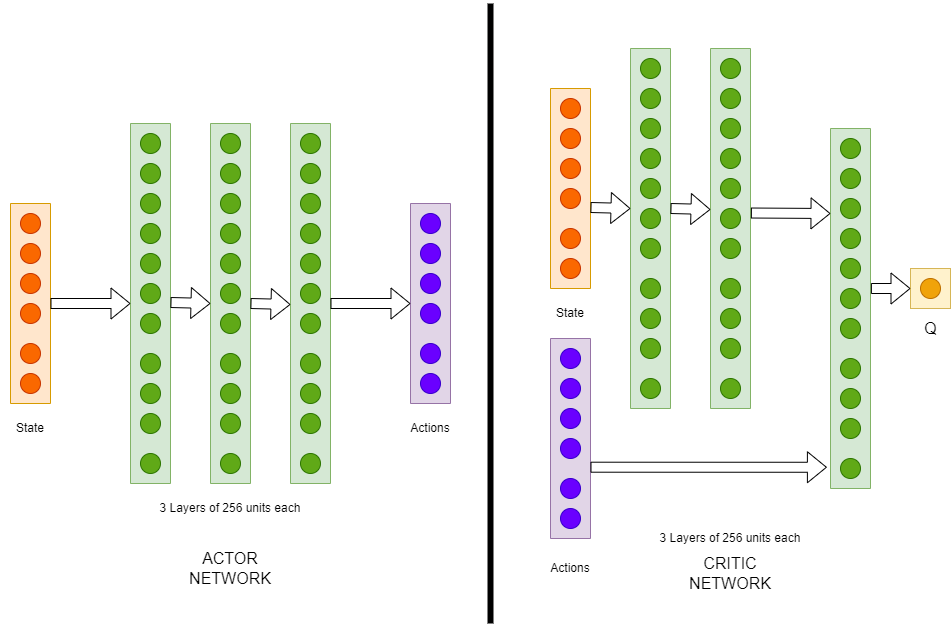
\includegraphics[width=1.0\textwidth]{images/ppo-network-v2.png}
    \caption{PPO Network Architecture}
    \label{fig:ppo-network}
\end{figure}

All the models were trained for 8-12 million steps depending on complexity. A batch size of 1024 was used with a buffer which stores experiences before making updates of the size 10240. All the agents were trained using 3 passes of the experience buffer to improve the stability of the training. Training episode ends when the reward accumulated becomes negative ($R \< 0$) or if the agent successfully completed a lap around track. At episode completion, the progress of the agent is reset on the track and the agent is reset at start location with 0 initial velocity. We use an initial learning rate of $3 \times 10^{-2}$ with a linear learning rate scheduler to ensure that the updates are not to large with the progress.

 % CONCLUSION AND FUTURE WORK
%  Chapter 6

\chapter{PERFORMANCE ANALYSIS}

In this chapter, we discuss the results obtained across the 3 phases
of our experimentation done as a part of this project.
\begin{itemize}
\item \textbf{Phase 1} covers the baseline scores obtained on all
  tracks
\item \textbf{Phase 2} covers the results obtained by performing
  Transfer Learning between tracks within the same level and across
  levels.
\item \textbf{Phase 3} is the final phase of our project which covers
  the result obtained by training the agents in the presence of the
  adversaries we have devised and the results obtained by transferring
  the knowledge learnt from these models.
\end{itemize}

For all these phases, we present the graphs obtained during the
training of our models. The first graphs shows the cumulative reward
obtained during the training process and our objective is to
\textit{maximise} the reward obtained. The second graphs shows the
average length of an episode of agent as the training
progresses. Having a lower value is \textit{better} but is not
mandatory as this is an indicator of how stable the agent is with
sudden dips indicating crashes on the track.

\section{PHASE I - BASELINE PERFORMANCE}
\subsection{Oval Track - Basic Track}
\begin{figure}[H]
    \centering
    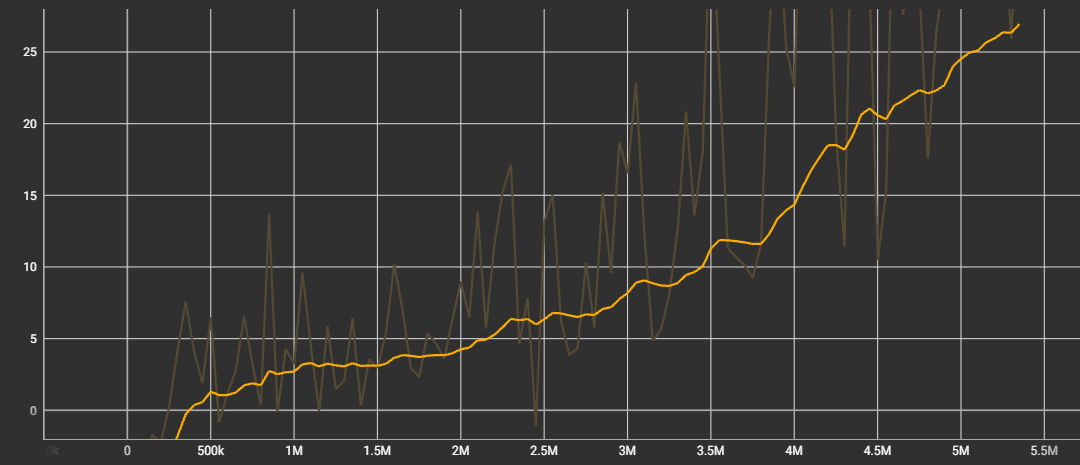
\includegraphics[width=1.0\textwidth]{images/graphs/OvalTrack-Reward.png}
    \caption{Oval Track Cumulative Reward. X-axis: Time steps. Y-axis: Cumulative Reward}
    \label{fig:1}
\end{figure}
\begin{figure}[H]
    \centering
    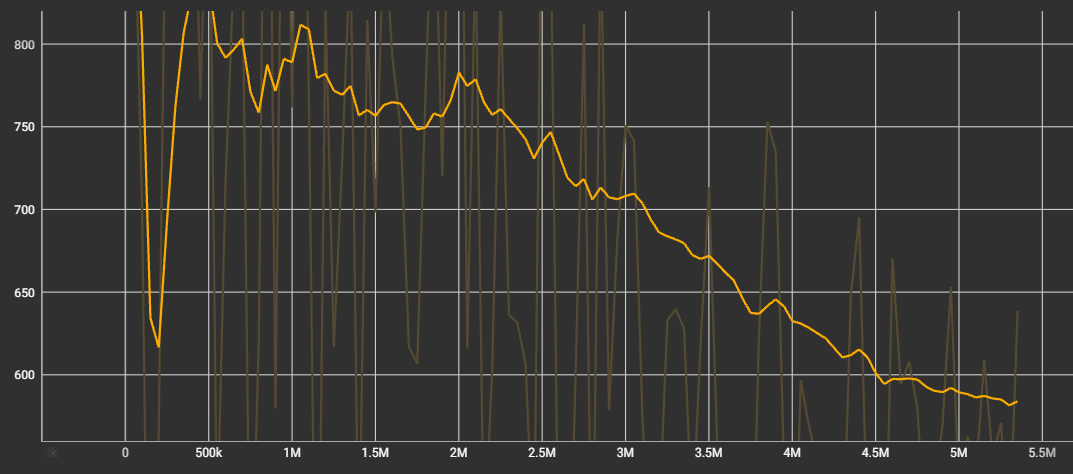
\includegraphics[width=1.0\textwidth]{images/graphs/OvalTrack-Episode.png}
    \caption{Oval Track Episode Length. X-axis: Time steps. Y-axis: Episode Length}
    \label{fig:2}
\end{figure}

\subsection{One-Kink Track}

\begin{figure}[H]
    \centering
    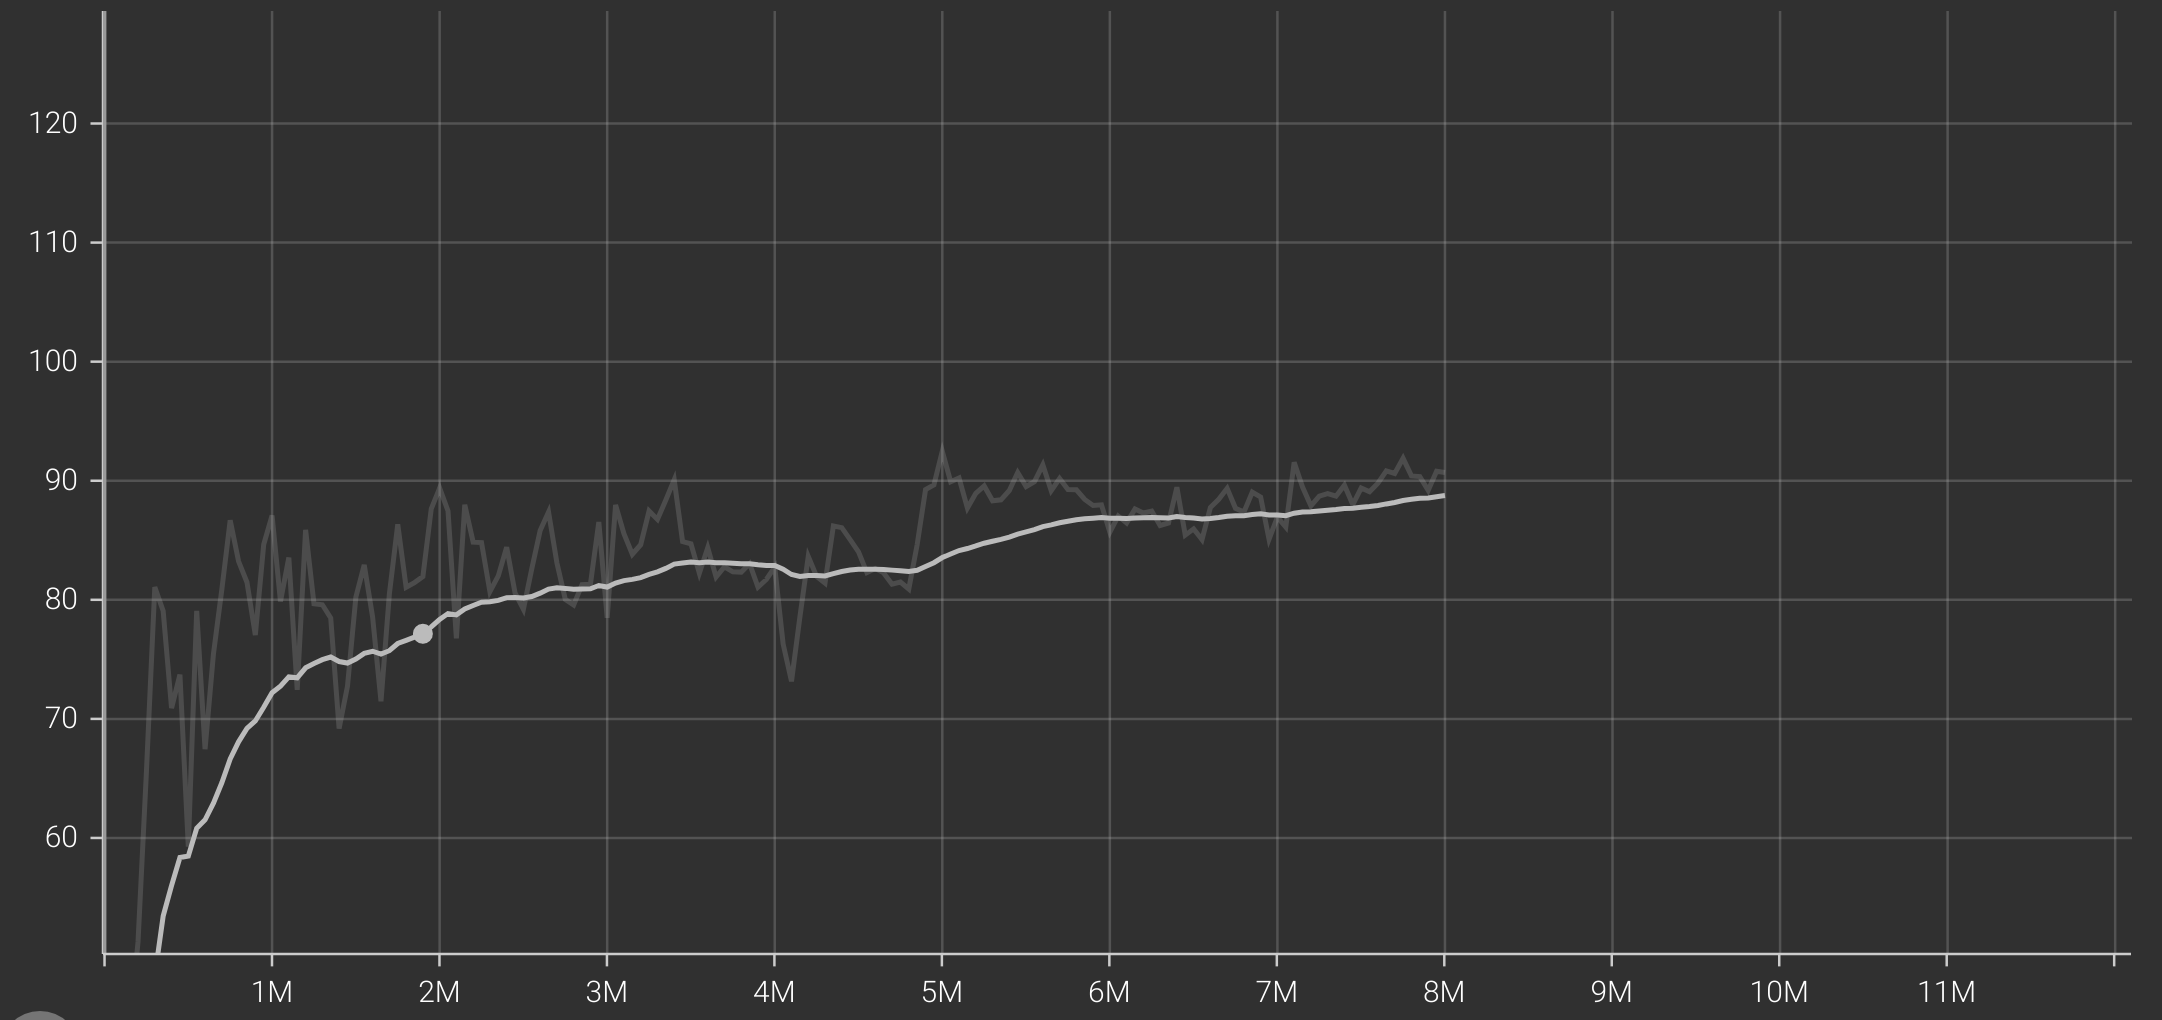
\includegraphics[width=1.0\textwidth]{images/graphs/OneKink-Reward.png}
    \caption{One Kink Track Cumulative Reward.  X-axis: Time steps  Y-axis: Cumulative Reward}
    \label{fig:3}
\end{figure}

\begin{figure}[H]
    \centering
    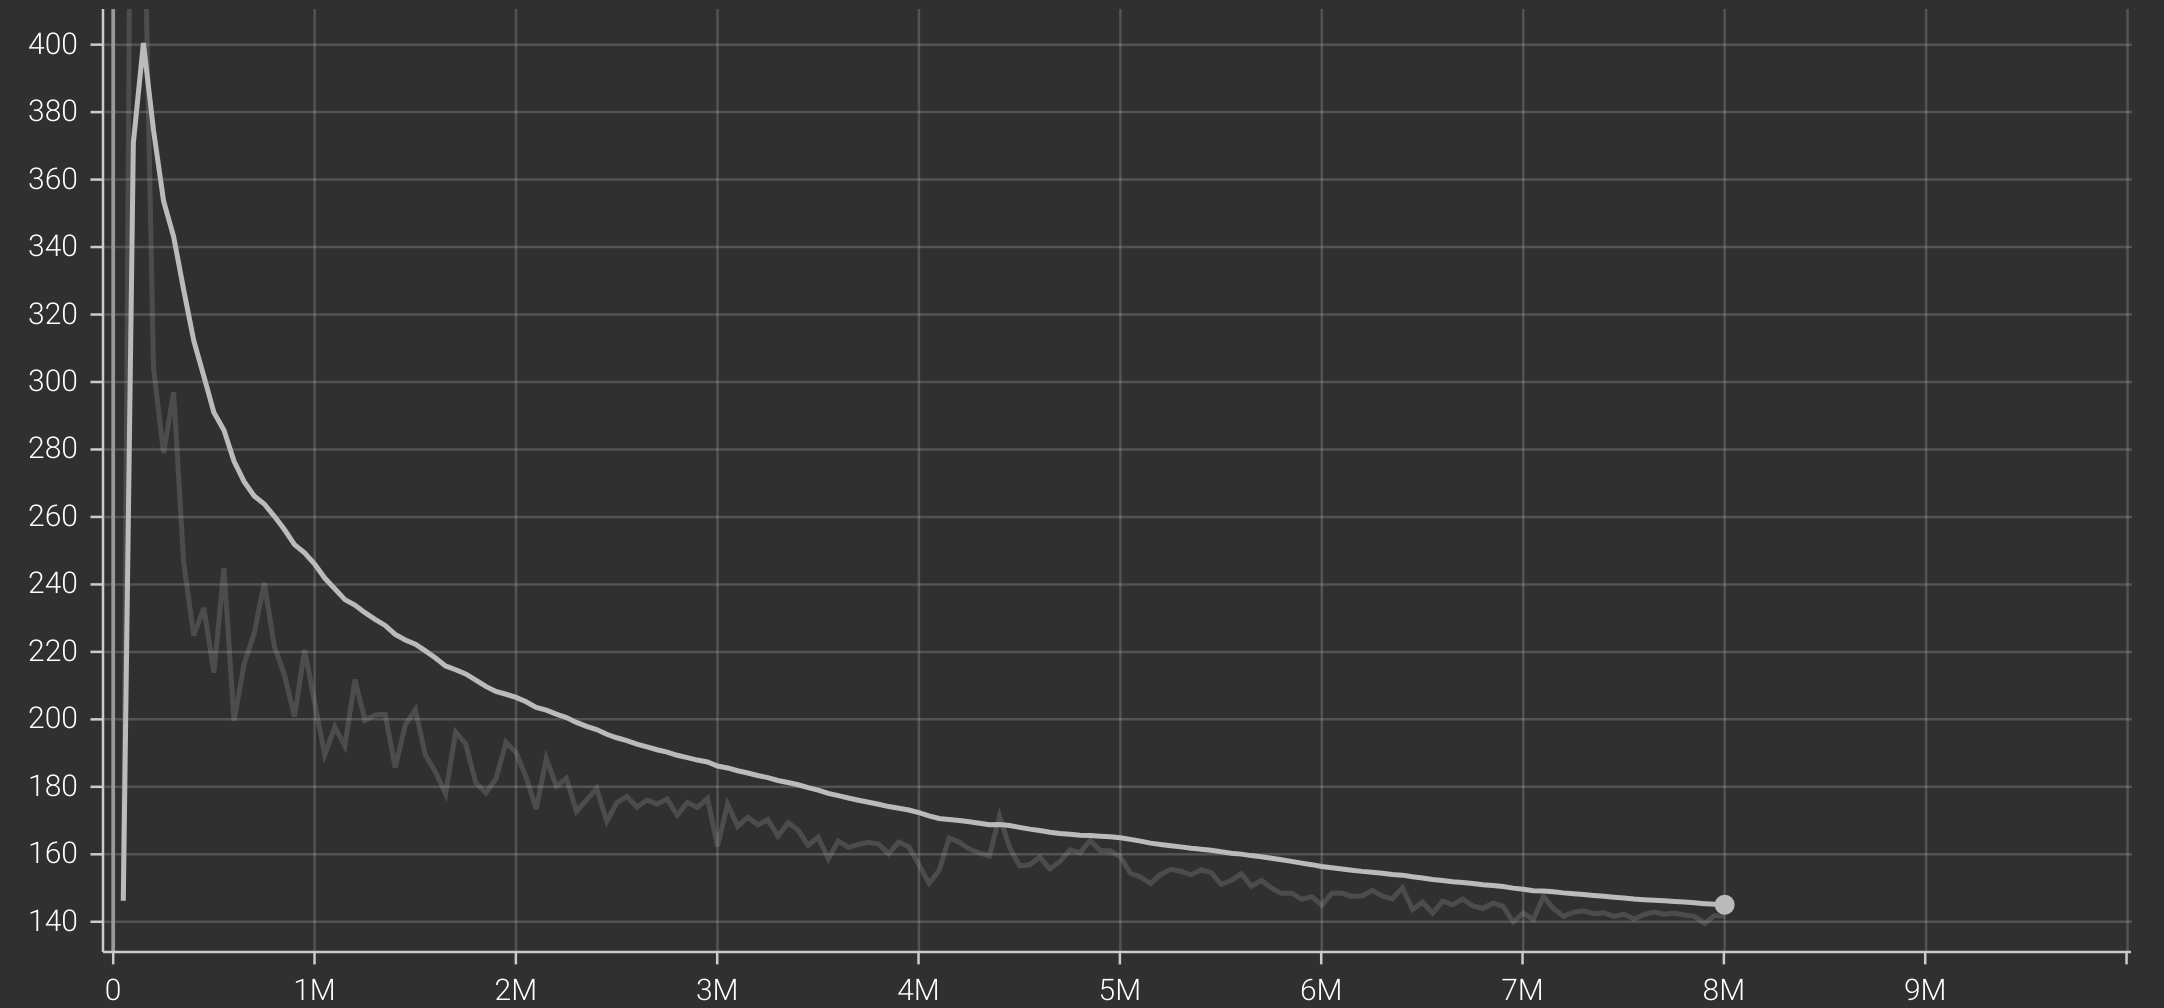
\includegraphics[width=1.0\textwidth]{images/graphs/OneKink-Episode.png}
    \caption{One Kink Track Episode Length.  X-axis: Time steps  Y-axis: Episode Length}
    \label{fig:4}
\end{figure}


\subsection{Two-Kink Track}

\begin{figure}[H]
    \centering
    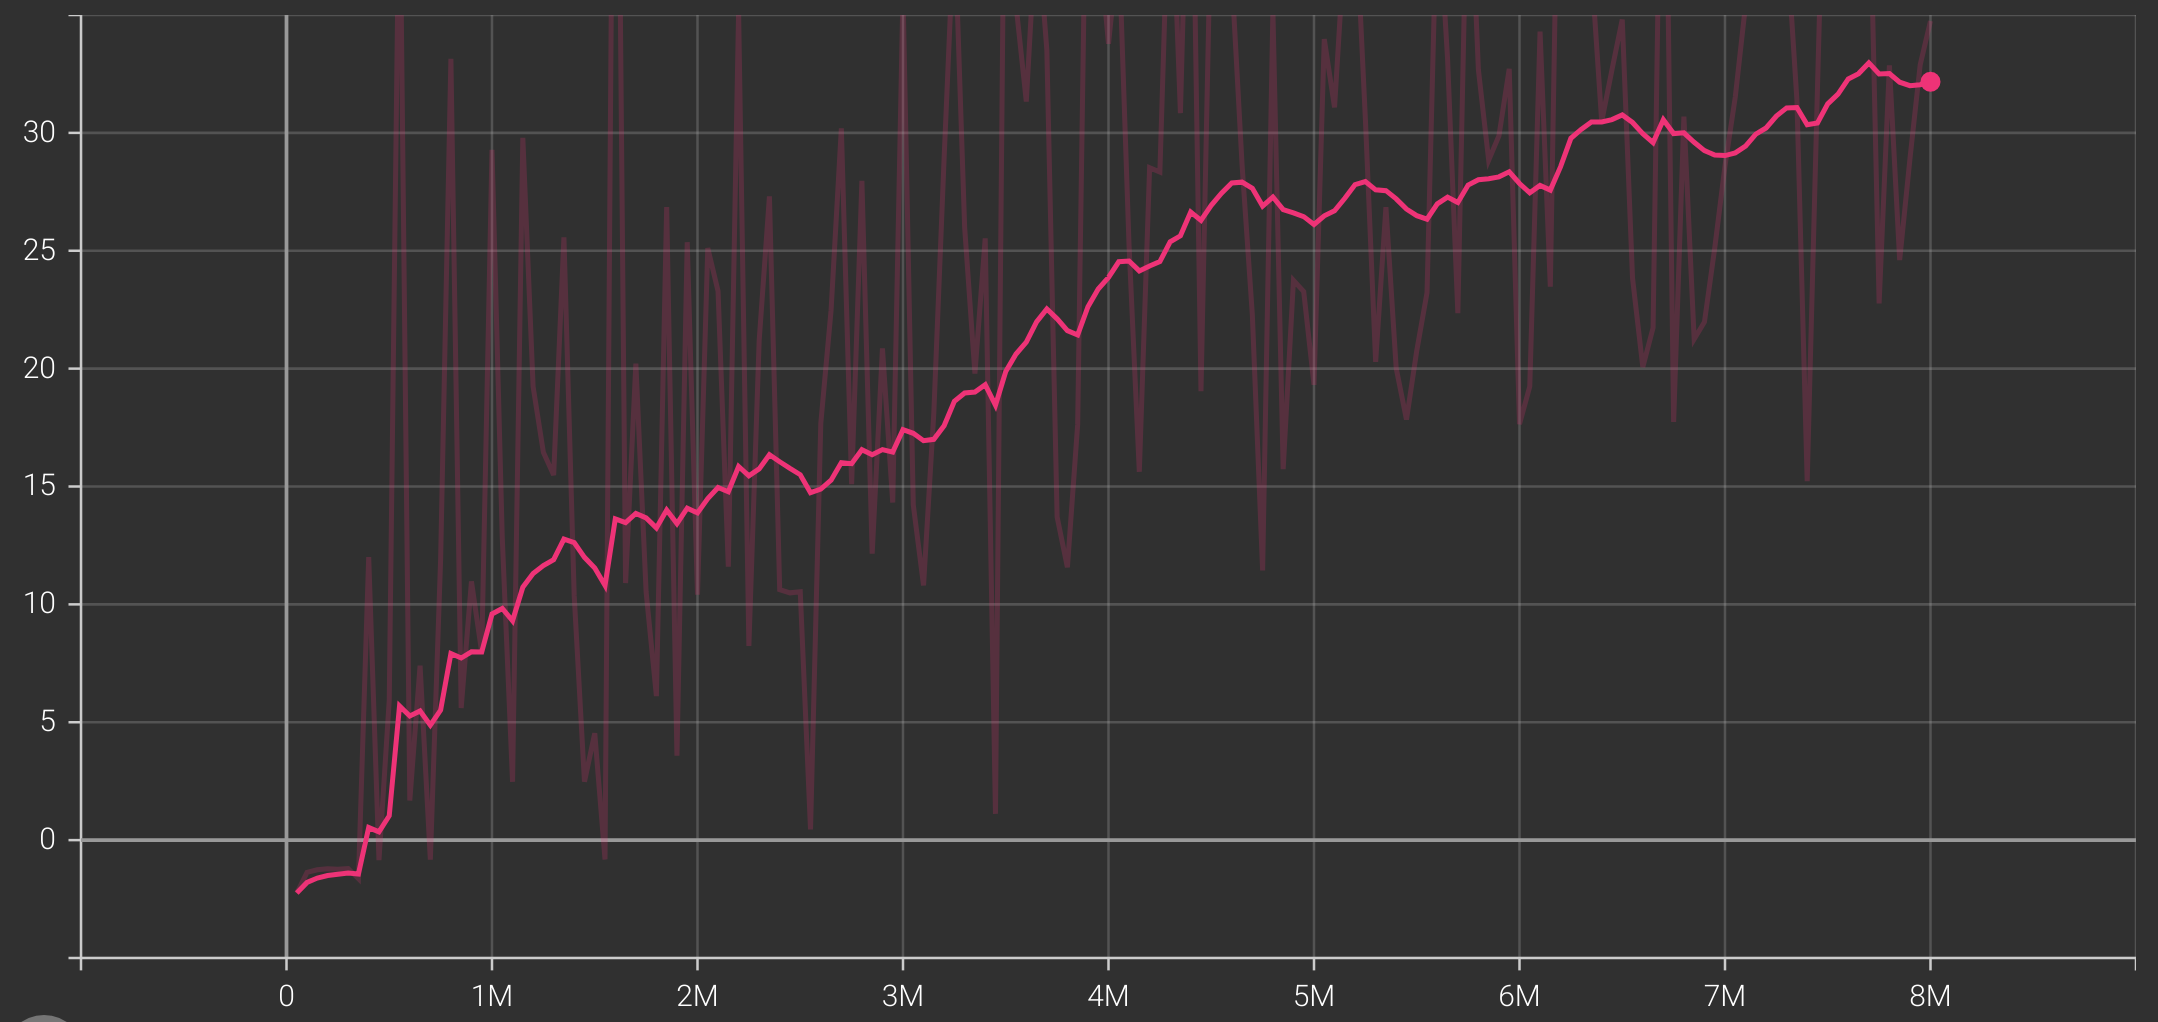
\includegraphics[width=1.0\textwidth]{images/graphs/TwoKink-Reward.png}
    \caption{Two Kink Track Cumulative Reward.  X-axis: Time steps  Y-axis: Cumulative Reward}
    \label{fig:5}
\end{figure}

\begin{figure}[H]
    \centering
    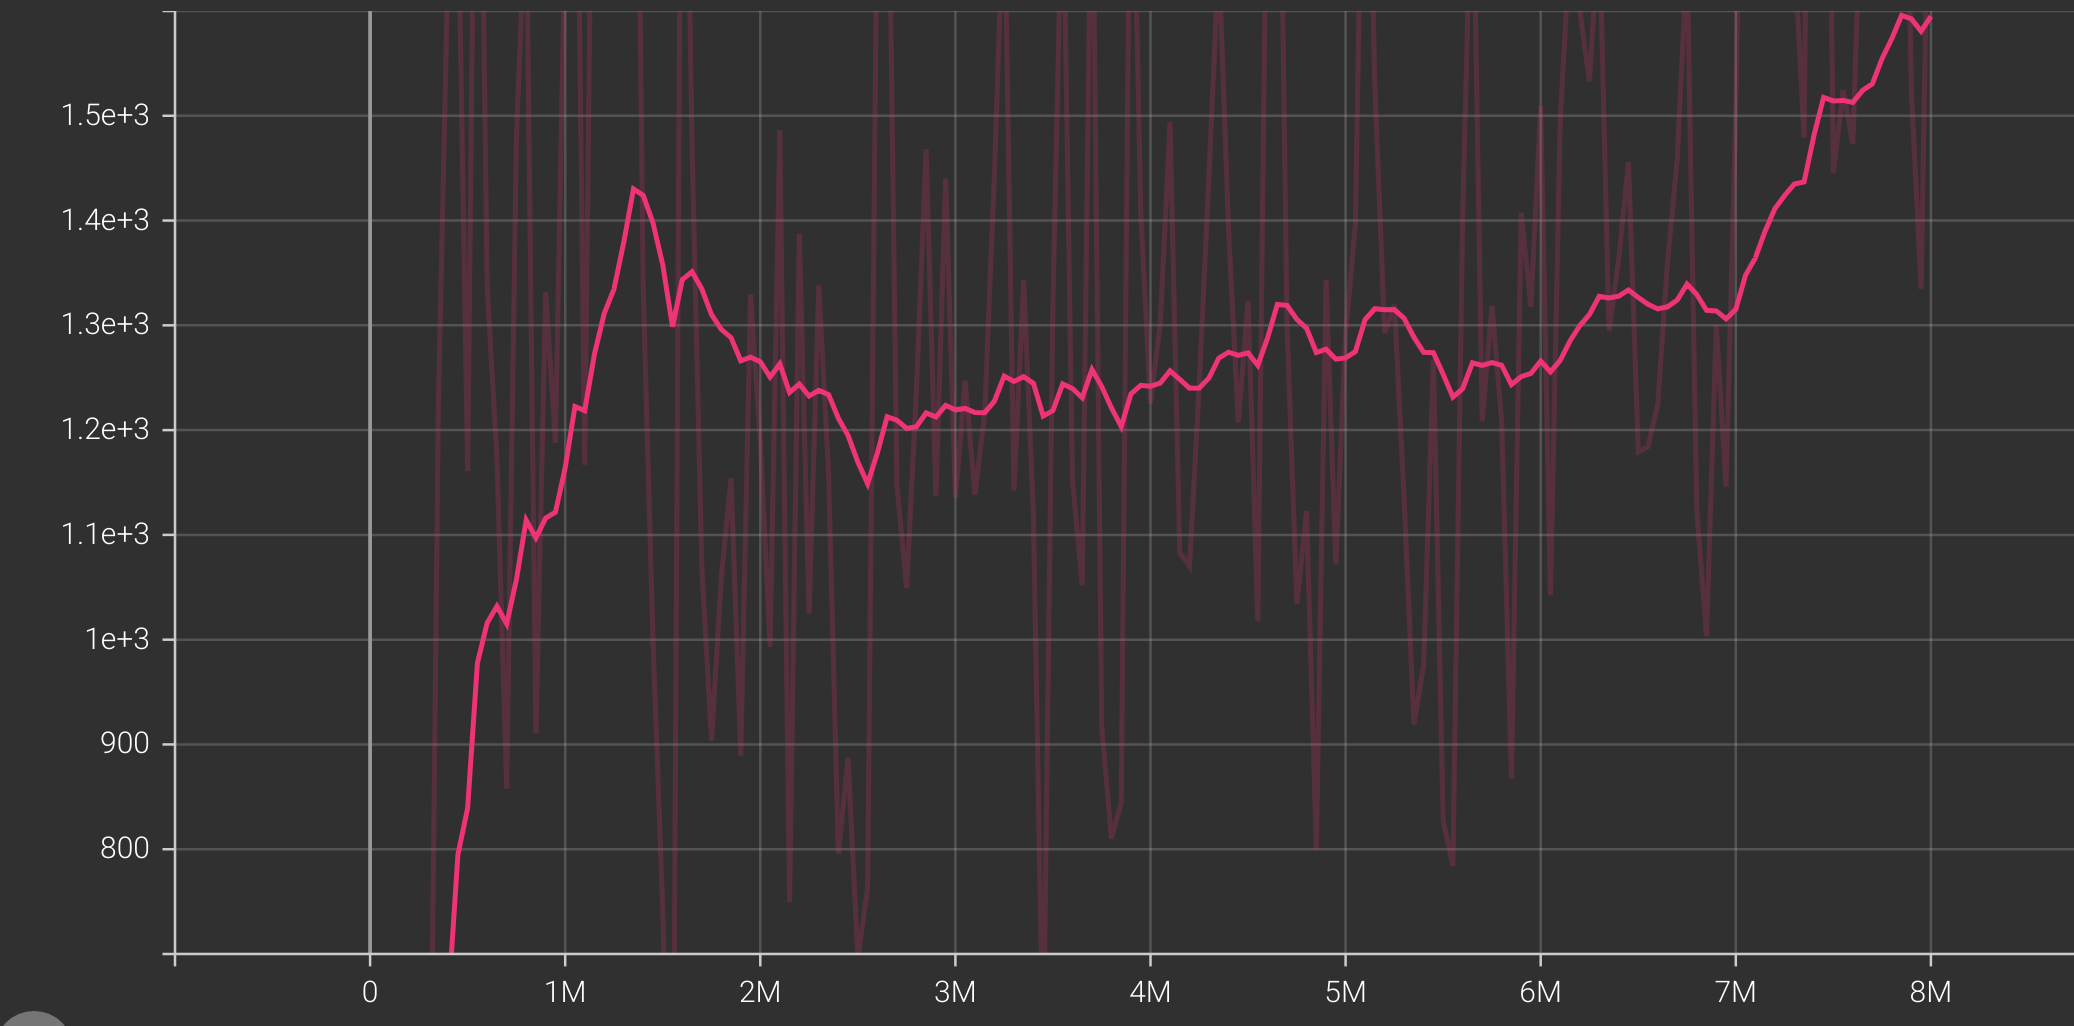
\includegraphics[width=1.0\textwidth]{images/graphs/TwoKink-Episode.png}
    \caption{Two Kink Track Episode Length.  X-axis: Time steps  Y-axis: Episode Length}
    \label{fig:6}
\end{figure}


\subsection{Barcelona}

\begin{figure}[H]
    \centering
    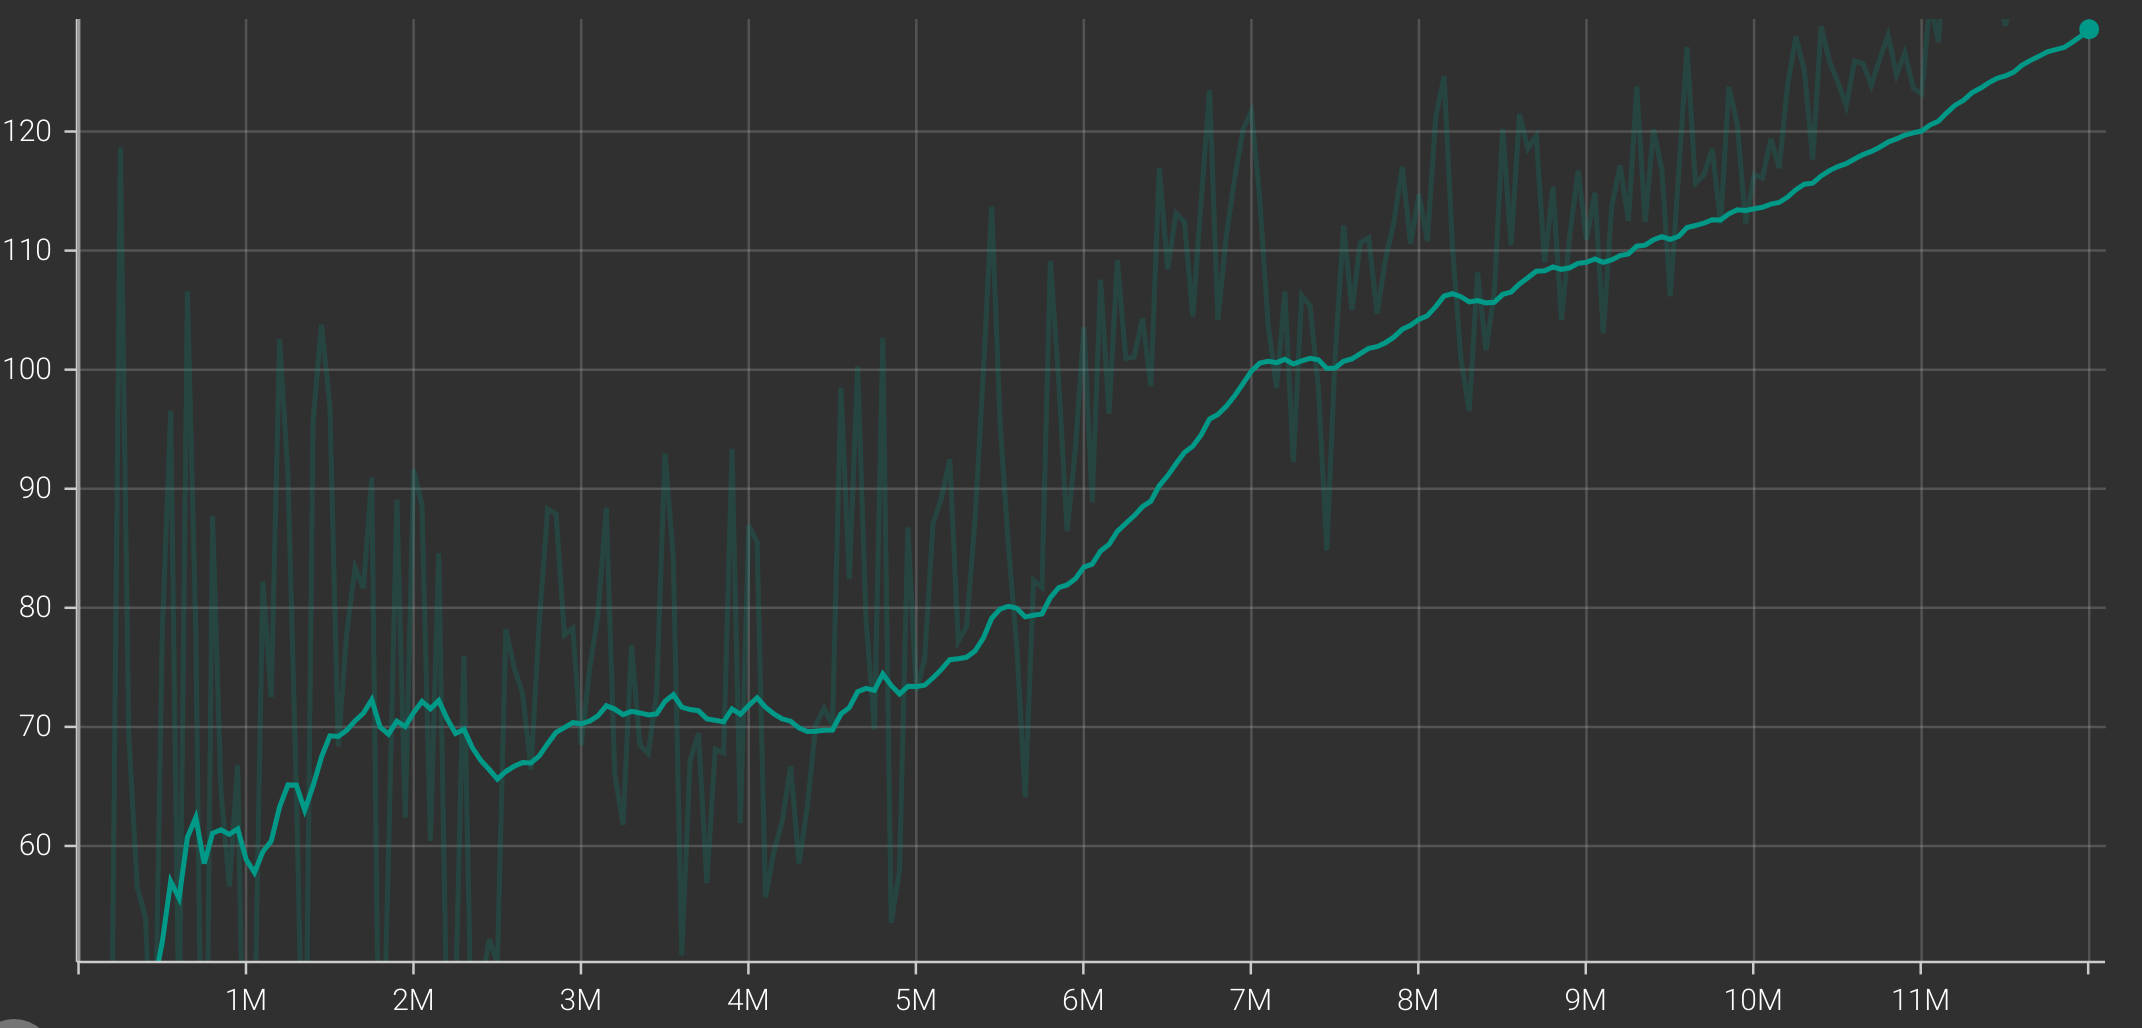
\includegraphics[width=1.0\textwidth]{images/graphs/Barcelona-Reward.png}
    \caption{Barcelona Track Cumulative Reward.  X-axis: Time steps  Y-axis: Cumulative Reward}
    \label{fig:7}
\end{figure}

\begin{figure}[H]
    \centering
    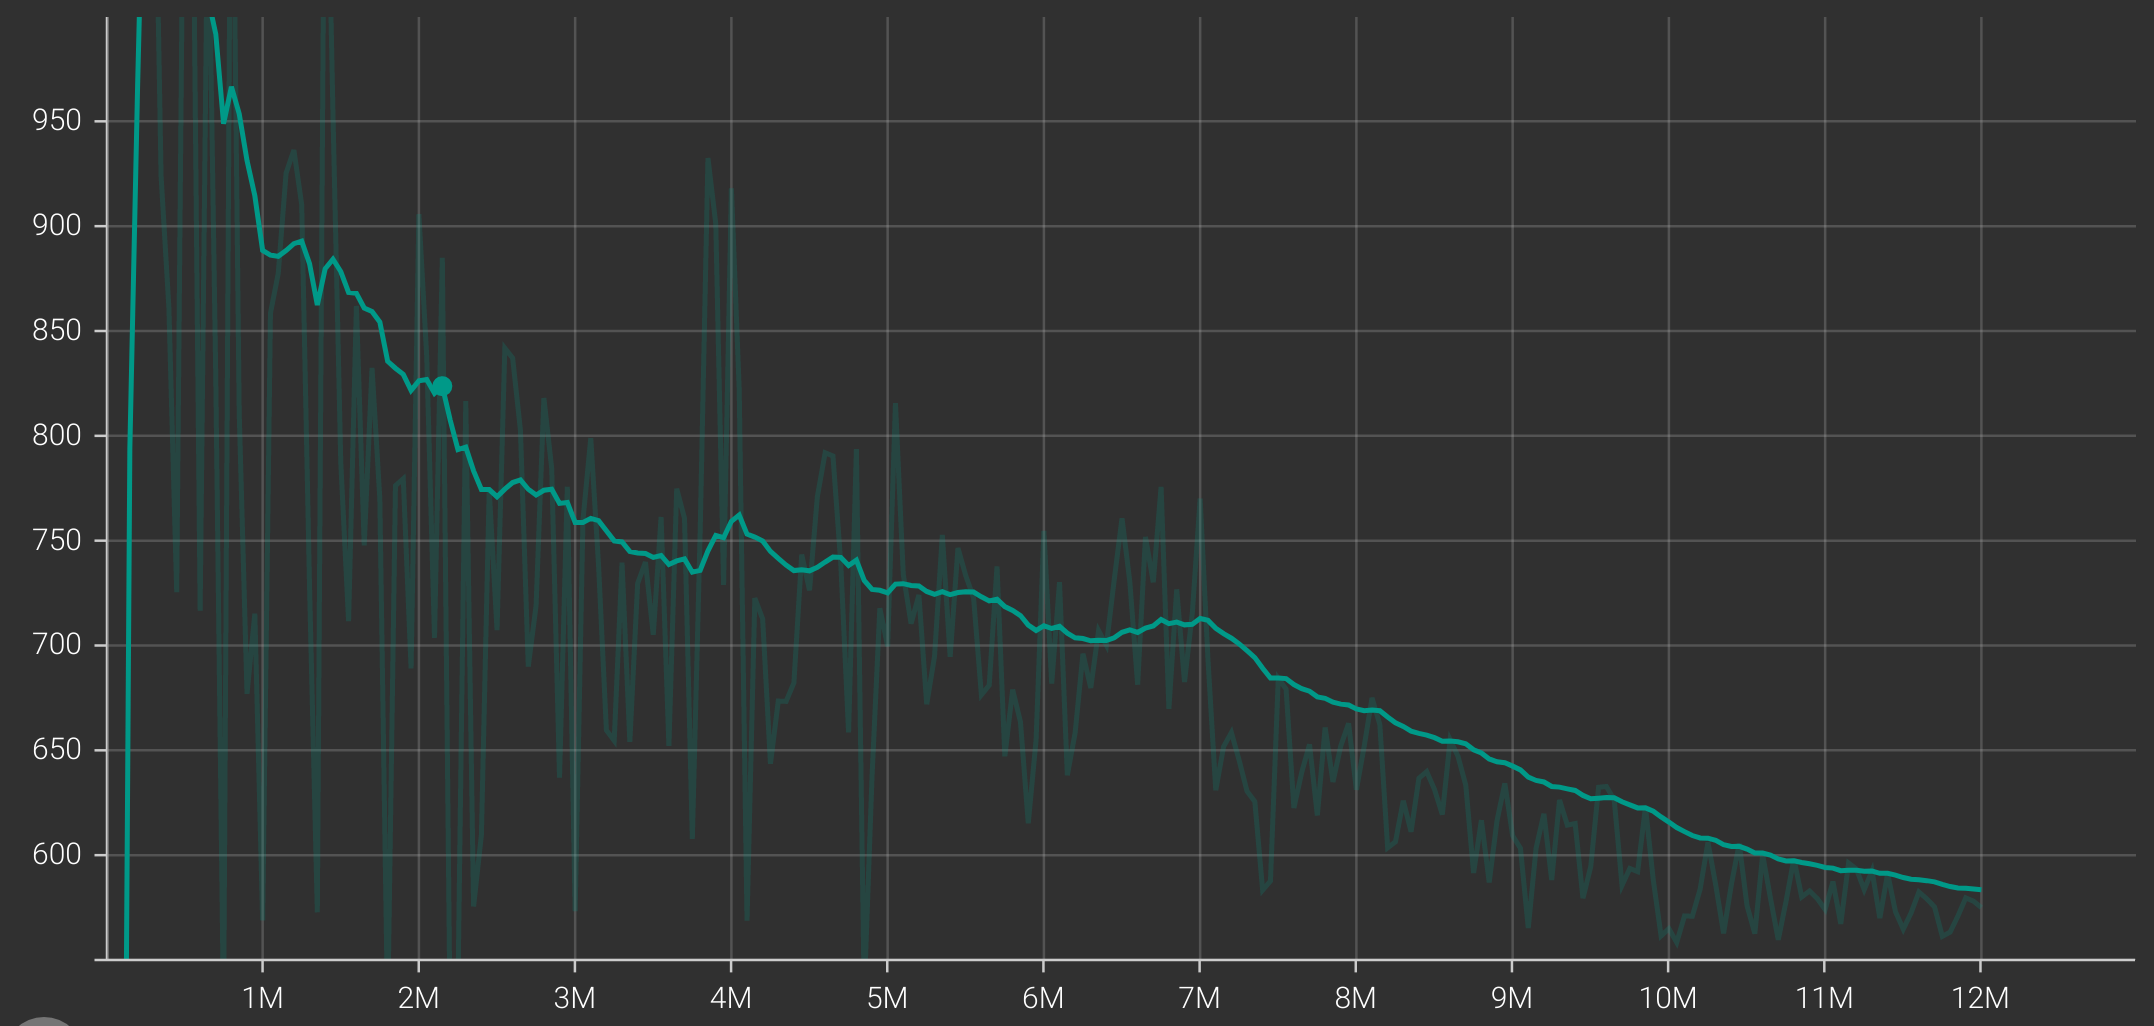
\includegraphics[width=1.0\textwidth]{images/graphs/Barcelona-Episode.png}
    \caption{Barcelona Track Episode Length.  X-axis: Time steps  Y-axis: Epsiode Length}
    \label{fig:8}
\end{figure}

\subsection{AWS Track}

\begin{figure}[H]
    \centering
    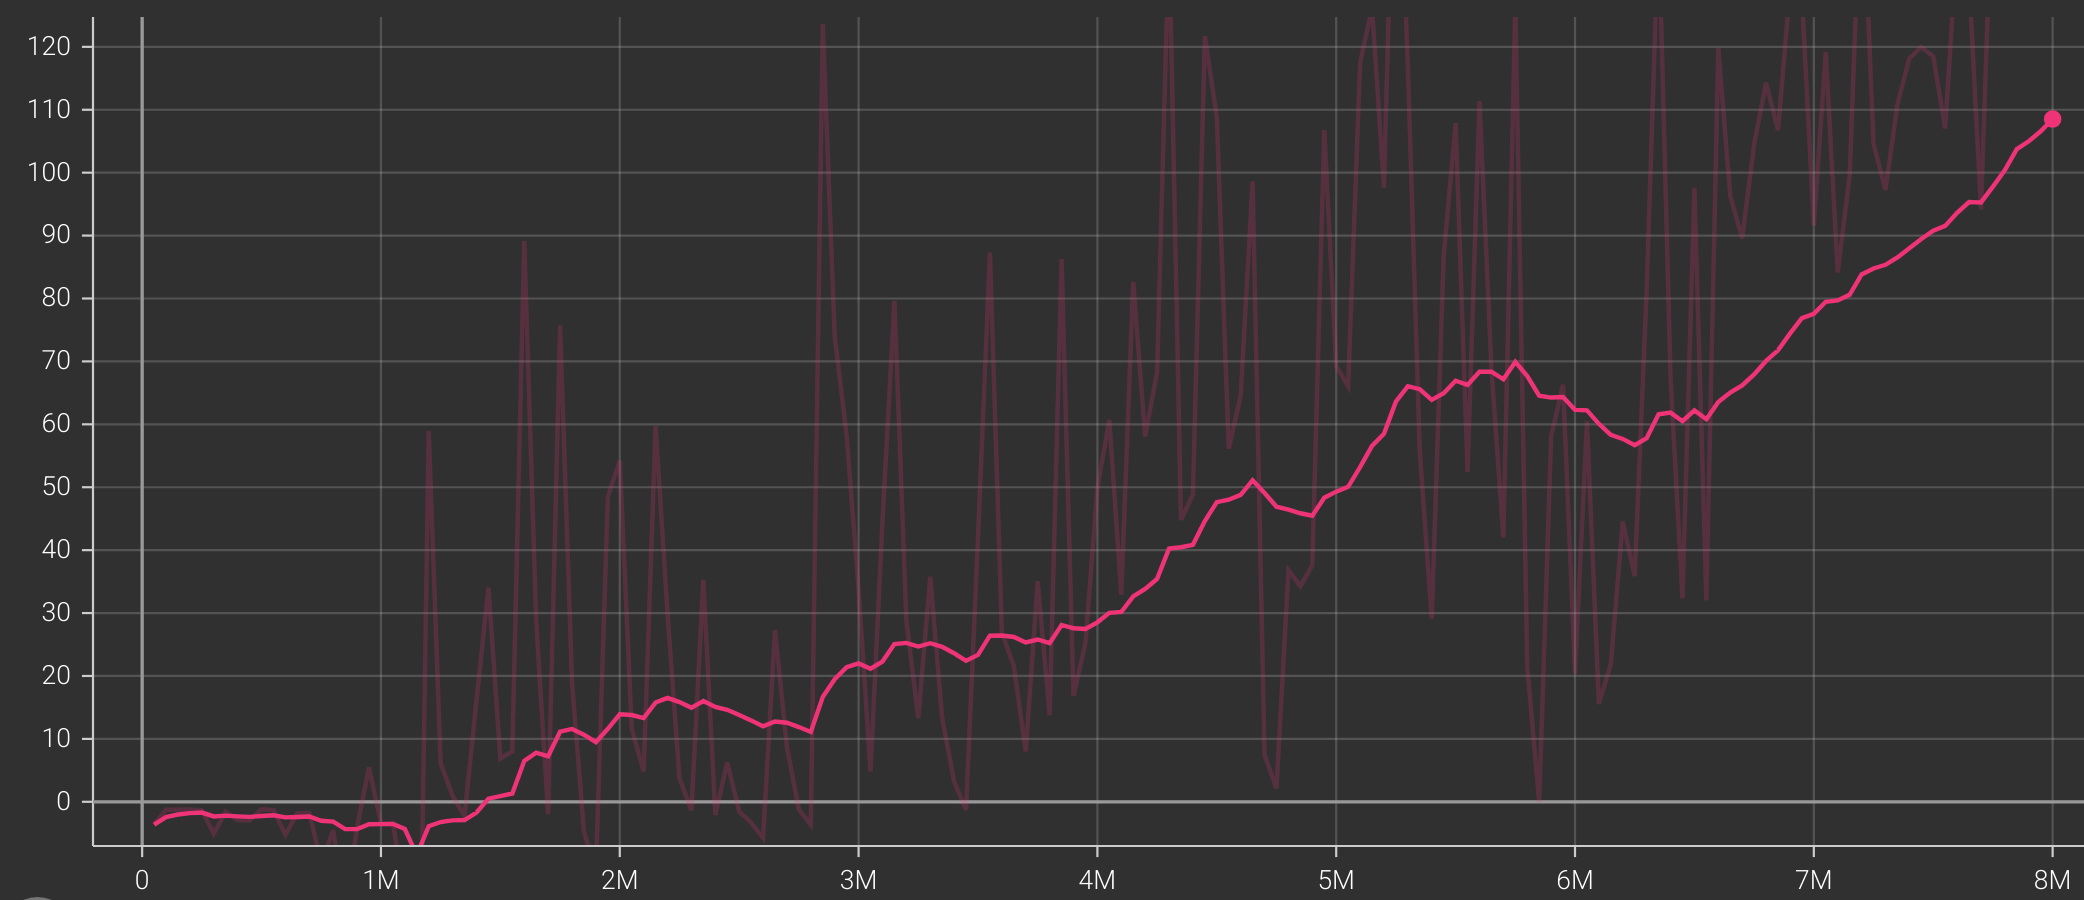
\includegraphics[width=1.0\textwidth]{images/graphs/AWS_baseline.png}
    \caption{AWS Track Cumulative Reward.  X-axis: Time steps  Y-axis: Cumulative Reward}
    \label{fig:9}
\end{figure}

\begin{figure}[H]
    \centering
    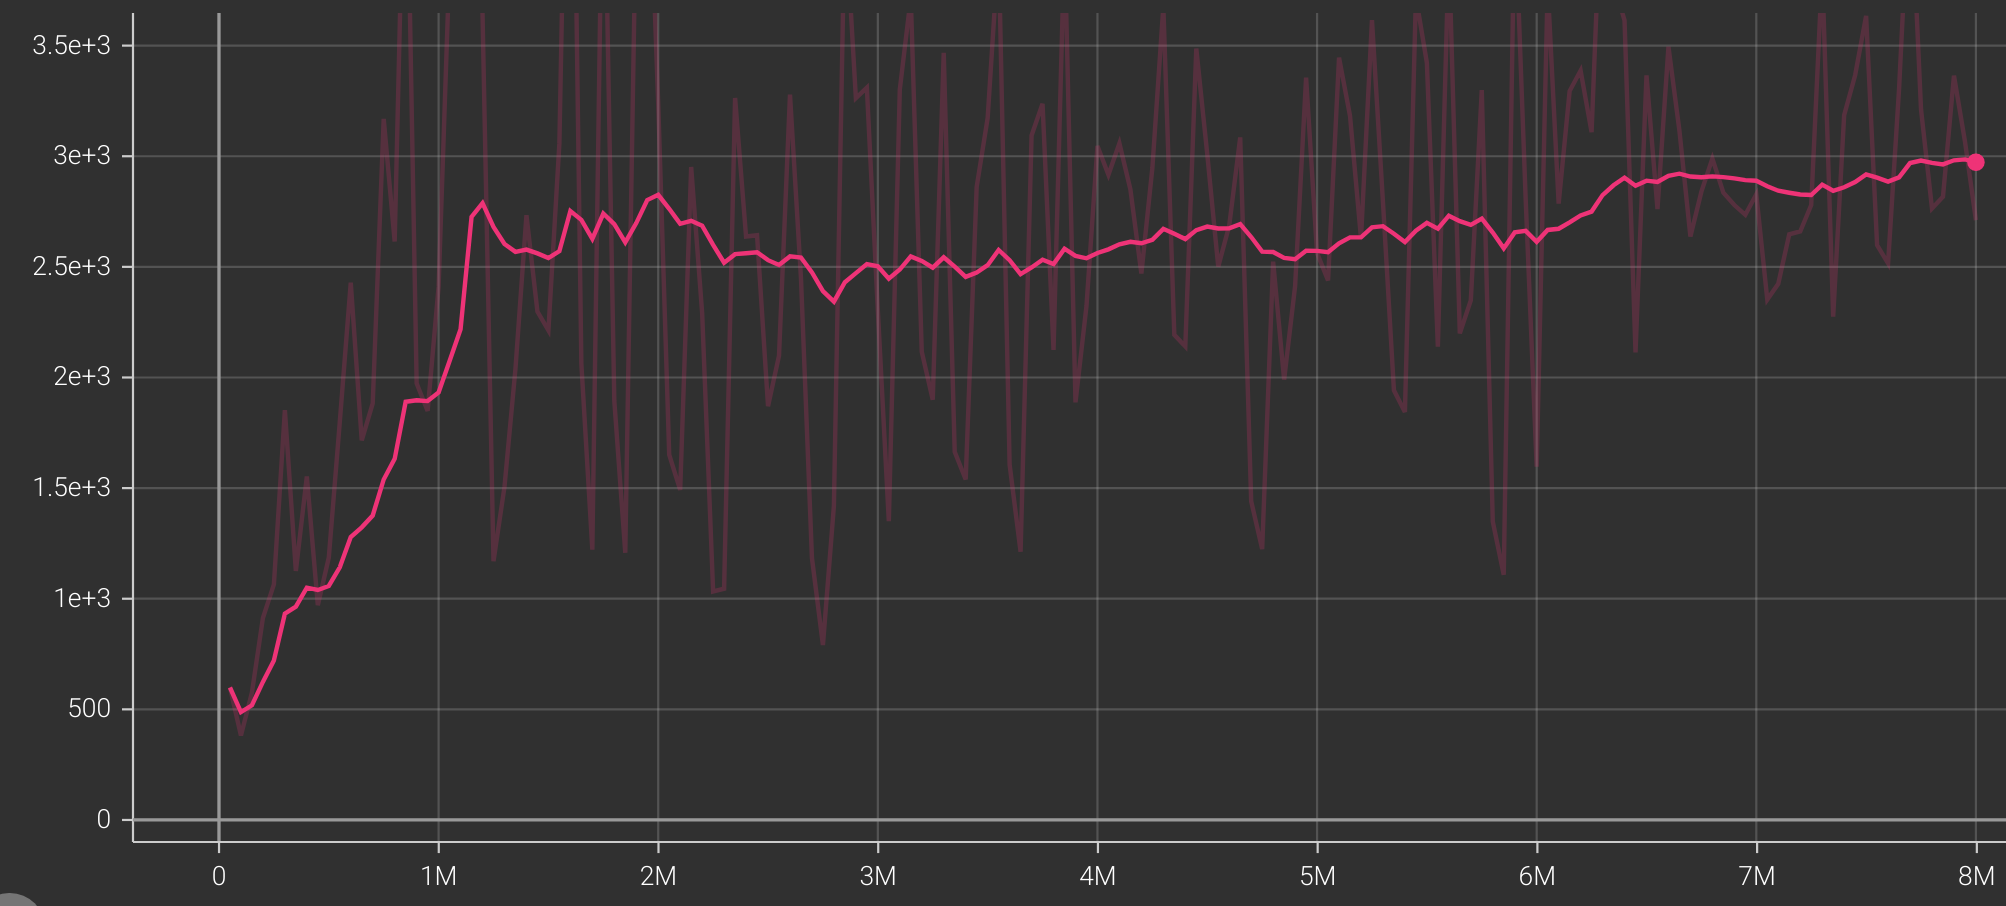
\includegraphics[width=1.0\textwidth]{images/graphs/AWS-EpisodeLength.png}
    \caption{AWS Track Cumulative Reward.  X-axis: Time steps  Y-axis: Episode Length}
    \label{fig:10}
\end{figure}

In this phase we record the baseline performance of the PPO algorithm
on all the tracks that we have developed in
Table~\ref{tab:baseline}. These scores will be used in the upcoming
sections to quantify the effects and improvement of Transfer Learning
and Adversarial Training.

\begin{table}[H]
\centering\begin{tabular}{|c|l|c|c|}
\hline
\textbf{Type}                                         & \textbf{Track} & \textbf{Steps (in Million)} & \textbf{Reward} \\ \hline
\multicolumn{1}{|c|}{\multirow{3}{*}{\textbf{Basic}}} & Oval Track     &  5                           &    41.2             \\ \cline{2-4} 
\multicolumn{1}{|c|}{}                                & One Kink       & 8                            &  90.7               \\ \cline{2-4} 
\multicolumn{1}{|c|}{}                                & Two Kink       & 8                           & 34.75           \\ \hline
\multirow{2}{*}{\textbf{Complex}}                     & Barcelona      & 12                         &   128.6              \\ \cline{2-4} 
                                                      & AWS Track      &        8                     & 136.8                 \\ \hline
\end{tabular}
\caption{Average reward scores of baseline models}
\label{tab:baseline}
\end{table}

\section{PHASE II - TRANSFER LEARNING}

\subsection{One-Kink -- Two-Kink TL Performance}

Here we compare the performance obtained by the model that uses
transfer learning in comparison to the baseline model of the Two-Kink
track with the source track (One-Kink) and target track (Two-Kink)
being tracks of the same class of complexity namely `Basic Tracks'.

\begin{figure}[H]
  \centering
  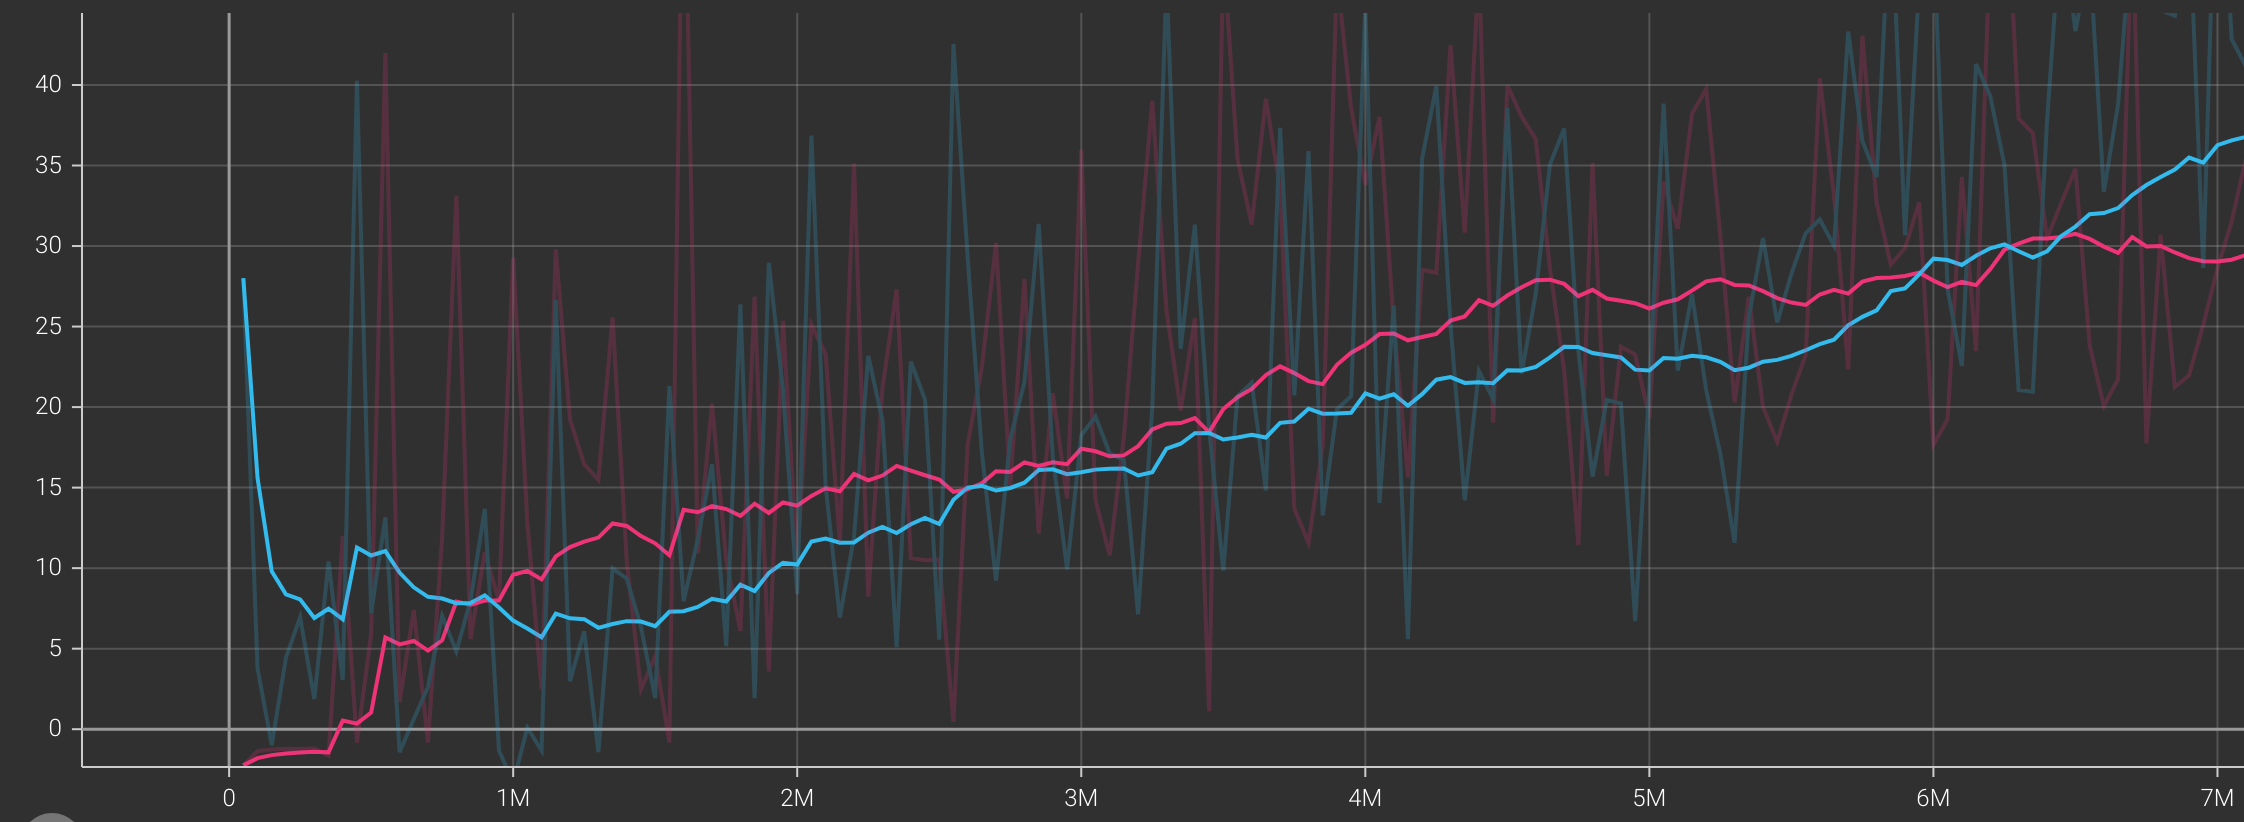
\includegraphics[width=1.0\textwidth]{images/graphs/TL-OneKink-TwoKink.png}
  \caption{\textit{Blue}: Transfer Learned model, \textit{Pink}:
    Baseline model. X-axis: Time steps. Y-axis: Cumulative Reward }
  \label{TL-OneKink-TwoKink}
\end{figure}
  
The graph in Figure~\ref{TL-OneKink-TwoKink} above represents the
rewards obtained with Transfer Learning and without Transfer Learning
on our Two-Kink Track. The Transfer Learned model was trained first on
the One-Kink track for 1 million steps and transferred for a further 7
million steps on the Two-Kink Track. Some key observations made are:
\begin{itemize}
\item The initial performance of the Transferred Model is higher as it
  has prior knowledge about the first few steps to be made which are
  track independent.
\item As the training further progresses, the scores obtained are very
  similar across both the models till the 6 million step mark.
\item The Transfer Learned model proceeds to performs better on the
  target task and achieves 13.1\% more reward (36.3 vs 32.1) at the
  end of TL training.
\item While the results are positive, Transfer Learning in RL is still
  more volatile than in the case of DL and ML. This is further
  highlighted by the similar performance of the two models.
\end{itemize}


\subsection{Two-Kink - AWS TL Performance}
In this experiment we perform transfer learning between tracks of two
levels of complexity. Two-Kink track is the most complex `Basic Track'
and AWS track is the most complicated track that we use in our
experimentation.
\begin{figure}[H]
  \centering
  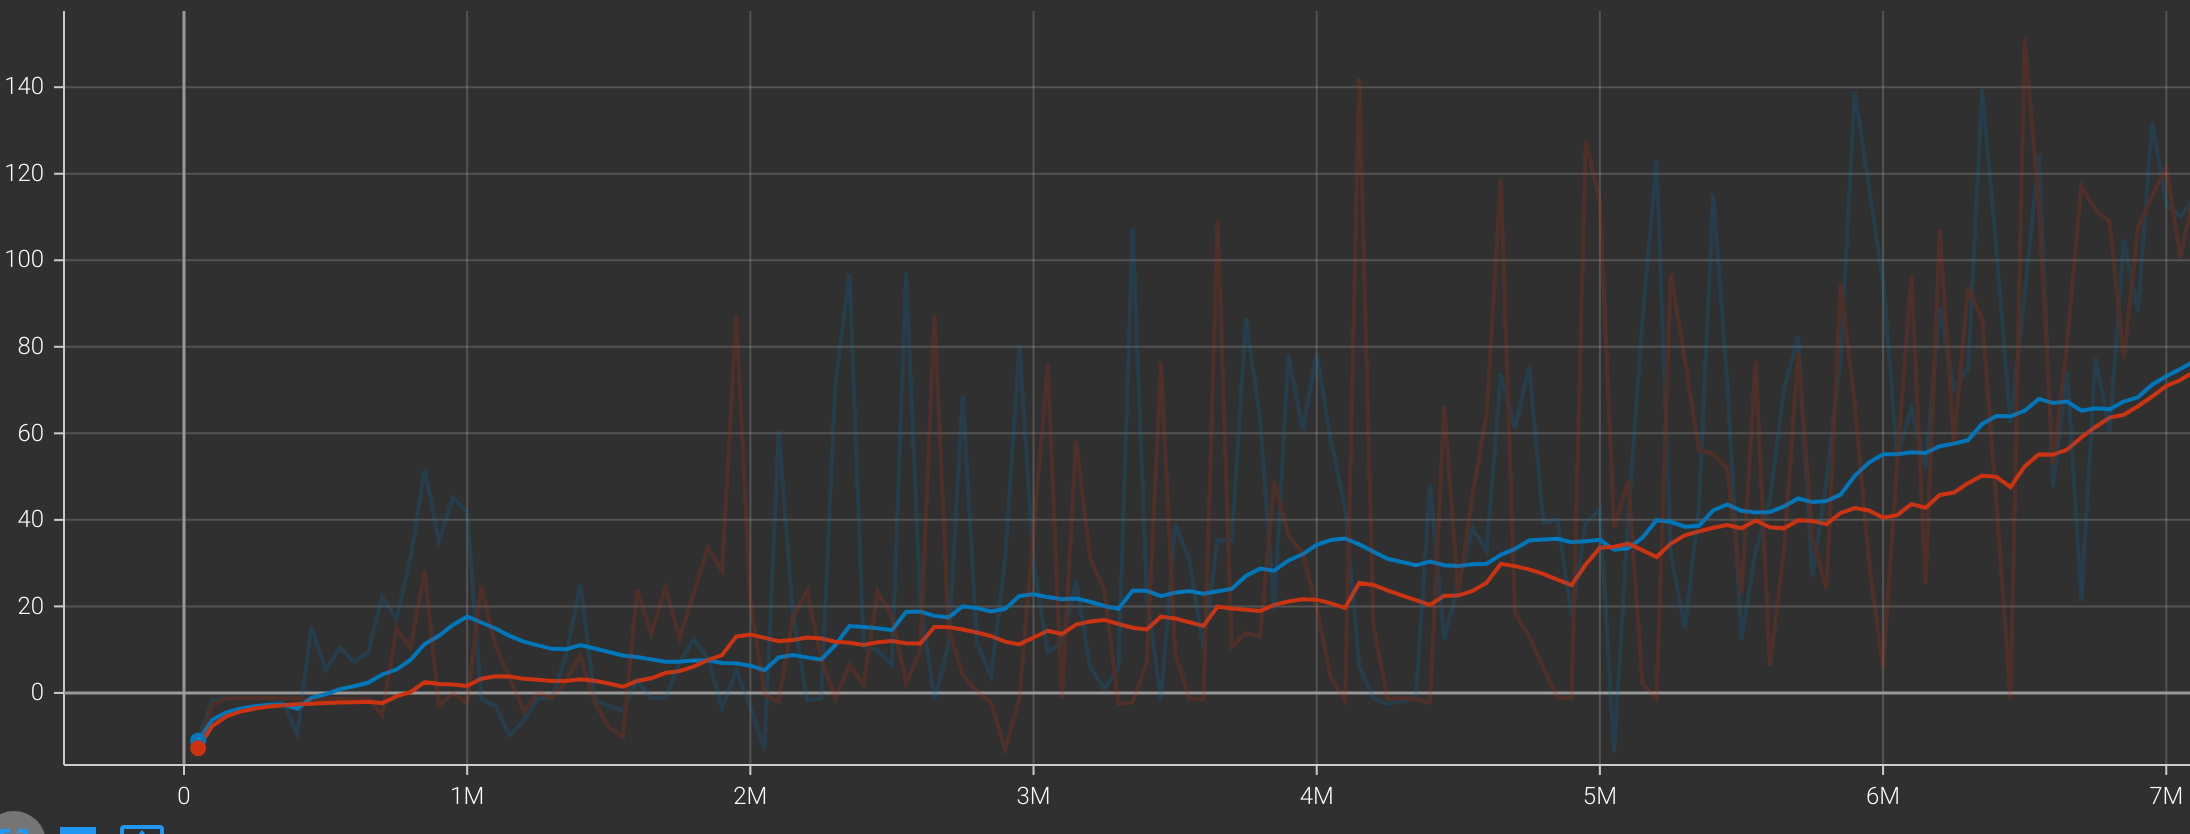
\includegraphics[width=1.0\textwidth]{images/graphs/TL-TwoKink-AWS.png}
  \caption{\textit{Blue}: Transfer Learned model, \textit{Red}:
    Baseline model. X-axis: Time steps. Y-axis: Cumulative Reward}
  \label{TL-TwoKink-AWS}
\end{figure}

The graph shown in Figure~\ref{TL-TwoKink-AWS} above represents the
rewards obtained with Transfer Learning and without Transfer Learning
on our AWS Track. The Transfer Learned model was trained first on the
Two-Kink track for 1 million steps and transferred for a further 7
million steps on the AWS Track. Some key observations made are
\begin{itemize}
\item The performance of the Transfer Learned model is consistently
  around 5-7\% better than the baseline model from the start of
  training.
\item Around the 6.5 million steps mark, the gap shrinks to a
  negligible difference with no significant improvement at the end of
  training
\end{itemize}
This further fortifies the findings that TL is much more challenging
in RL than in DL or ML.


\section{PHASE III}

\subsection{Transfer Learning after Adversarial Training }
In this section, we shall explore the effects and results of
performing Adversarial Training. We shall discuss its effects on
transfer learning between two tracks of similar complexity (One-Kink
track and Two-Kink track), and between tracks of varying complexity
(Two-Kink Track and AWS Track).  We are using 2 different types of
random noise attacks: Adversarial attack on the Observations (AT-TL)
and the Adversarial Attack on the actions (AAT-TL)

\subsubsection{One Kink to Two Kink}

\begin{figure}[H]
  \centering
  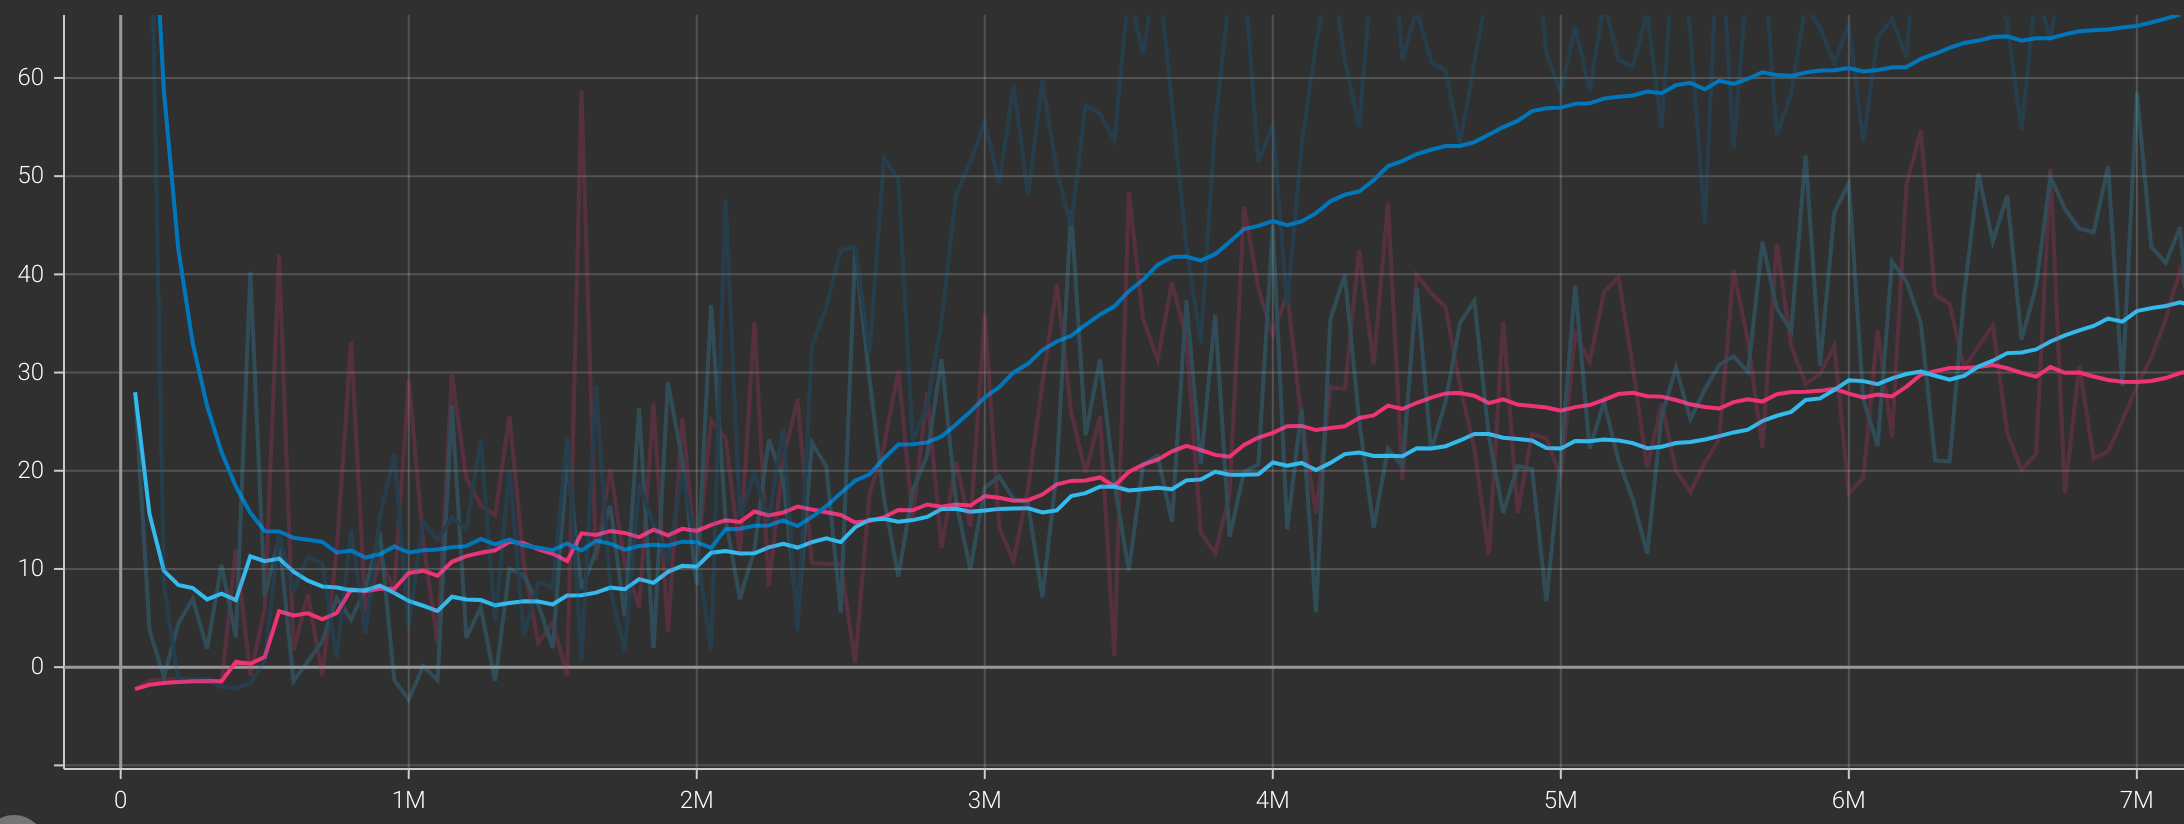
\includegraphics[width=1.0\textwidth]{images/graphs/AT-TL-OneKink-TwoKink.png}
  \caption{\textit{Dark-Blue}: Adversarially Trained(Observation
    Attack) Transfer Learned model, \textit{Light-Blue}: Transfer
    Learned model, \textit{Red}: Baseline model. X-axis: Time
    steps. Y-axis: Cumulative Reward }
  \label{fig:my_label}
\end{figure}

% The adversarial attack performed in this model is a random noise attack, which perturbs the sensory inputs of the model by moving the next checkpoint by a small distance.
% The above graph shows the model performance of the Adversarial trained - transfer learned model, compared to the simple transfer learned and baseline model. In this graph we can clearly see the advantage of using adversarial training. For the same number of steps the Adversarial trained model outperforms the other two models by a significant margin. 

\begin{figure}[H]
  \centering
  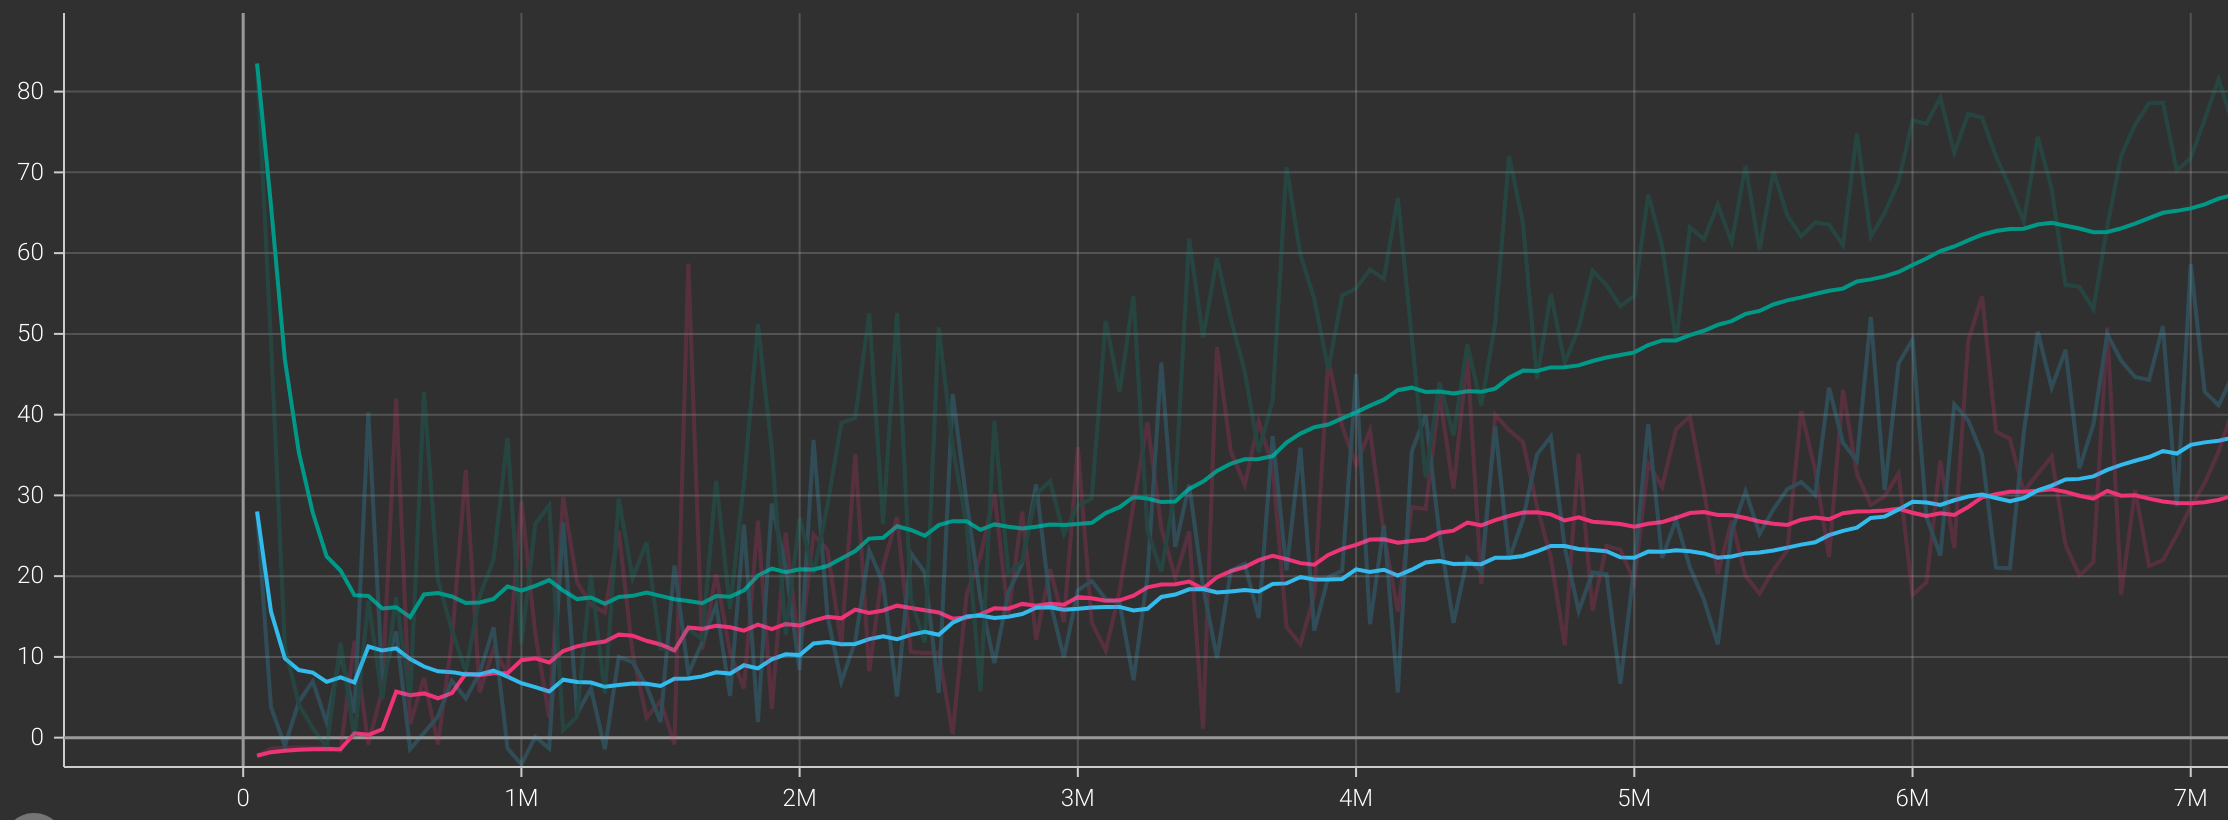
\includegraphics[width=1.0\textwidth]{images/graphs/AAT2-TL-OneKInk-TwoKink.png}
  \caption{\textit{Green}: Adversarially trained(Action Attack)
    transfer learned model, \textit{Light-Blue}: Transfer Learned
    model, \textit{Red}: Baseline model. X-axis: Time steps. Y-axis:
    Cumulative Reward }
  \label{fig:my_label}
\end{figure}

% This graph shows the performance of the model that is trained with an action adversary. Again we observe that the adversarial training followed by transfer learning improves the performance of the model/agent by a significant margin when compared to simple transfer learning.

% We can see that performing Adversarial Training followed by Transfer learning in both cases seems to be very effective; this may be attributed to the similarity of the layout of the tracks. The agent is able to better learn the state representations when we use adversarial training. The agent is able to use prior knowledge because of the higher quality of representations learned as a result of the adversarial training as we hypothesized. 

Various Action Adversary Models were trained using different action
adversary thresholds. It was observed that values are between 0.2 to
0.5; we see a significant drop in performance when $threshold > 0.6$.
\begin{itemize}
\item The AT model reaches an average reward of 65.3 at 7 million
  steps, which is is significantly better than the Transfer Learning
  model (36.3).
\item This is a 79.9\% improvement over the average reward obtained by
  the simple Transfer learned model.
\item We also observe that the AAT model is similar in performance to
  the AT model and reaches a score of 65.5 at the end of 7 million
  steps.
\item This is again a 80.4\% improvement over the simple Transfer
  learned model.
\end{itemize}
We can see that performing Adversarial Training followed by Transfer
learning in both cases seems to be extremely effective; this may be
attributed to the similarity of the layout of the tracks. The agent is
able to better learn the state representations when we use adversarial
training and is thus performing better after transfer learning.


\subsubsection{Two Kink to AWS }

\begin{figure}[H]
  \centering
  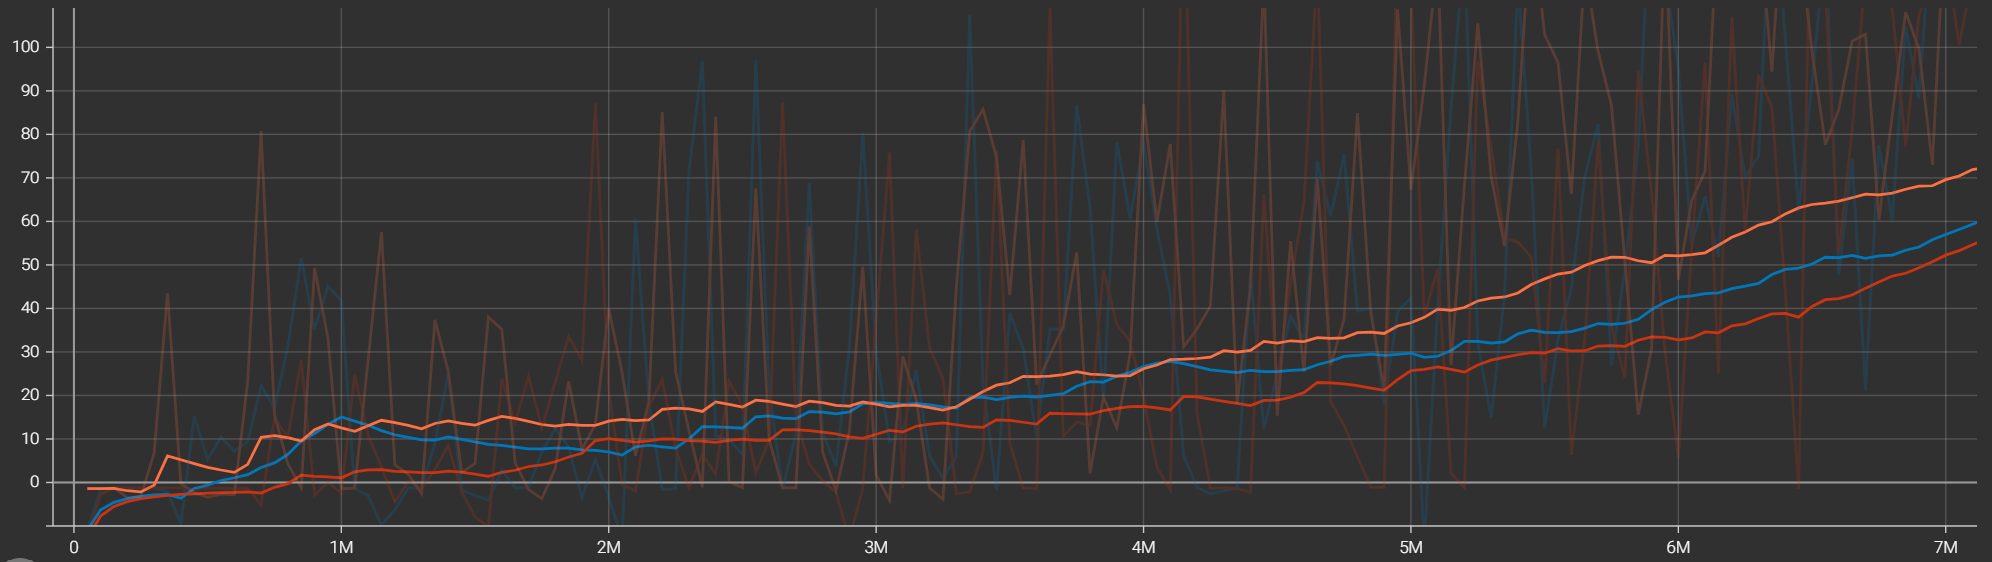
\includegraphics[width=0.9\textwidth]{images/graphs/AT-TL-TwoKink-AWSTrack-0.98.png}
  \caption{\textit{Orange}: Adversarially Trained(Observation Attack)
    Transfer Learned model, \textit{Blue}: Transfer Learned model,
    \textit{Red}: Baseline model. X-axis: Time steps. Y-axis:
    Cumulative Reward }
  \label{fig:my_label}
\end{figure}

% In this graph we can observe that the results produced by the observation adversary trained transfer learned model(AT-TL) performs better that the baseline model and the transfer learned model. The AT-TL model uses adversarial training that disrupts

\begin{figure}[H]
  \centering
  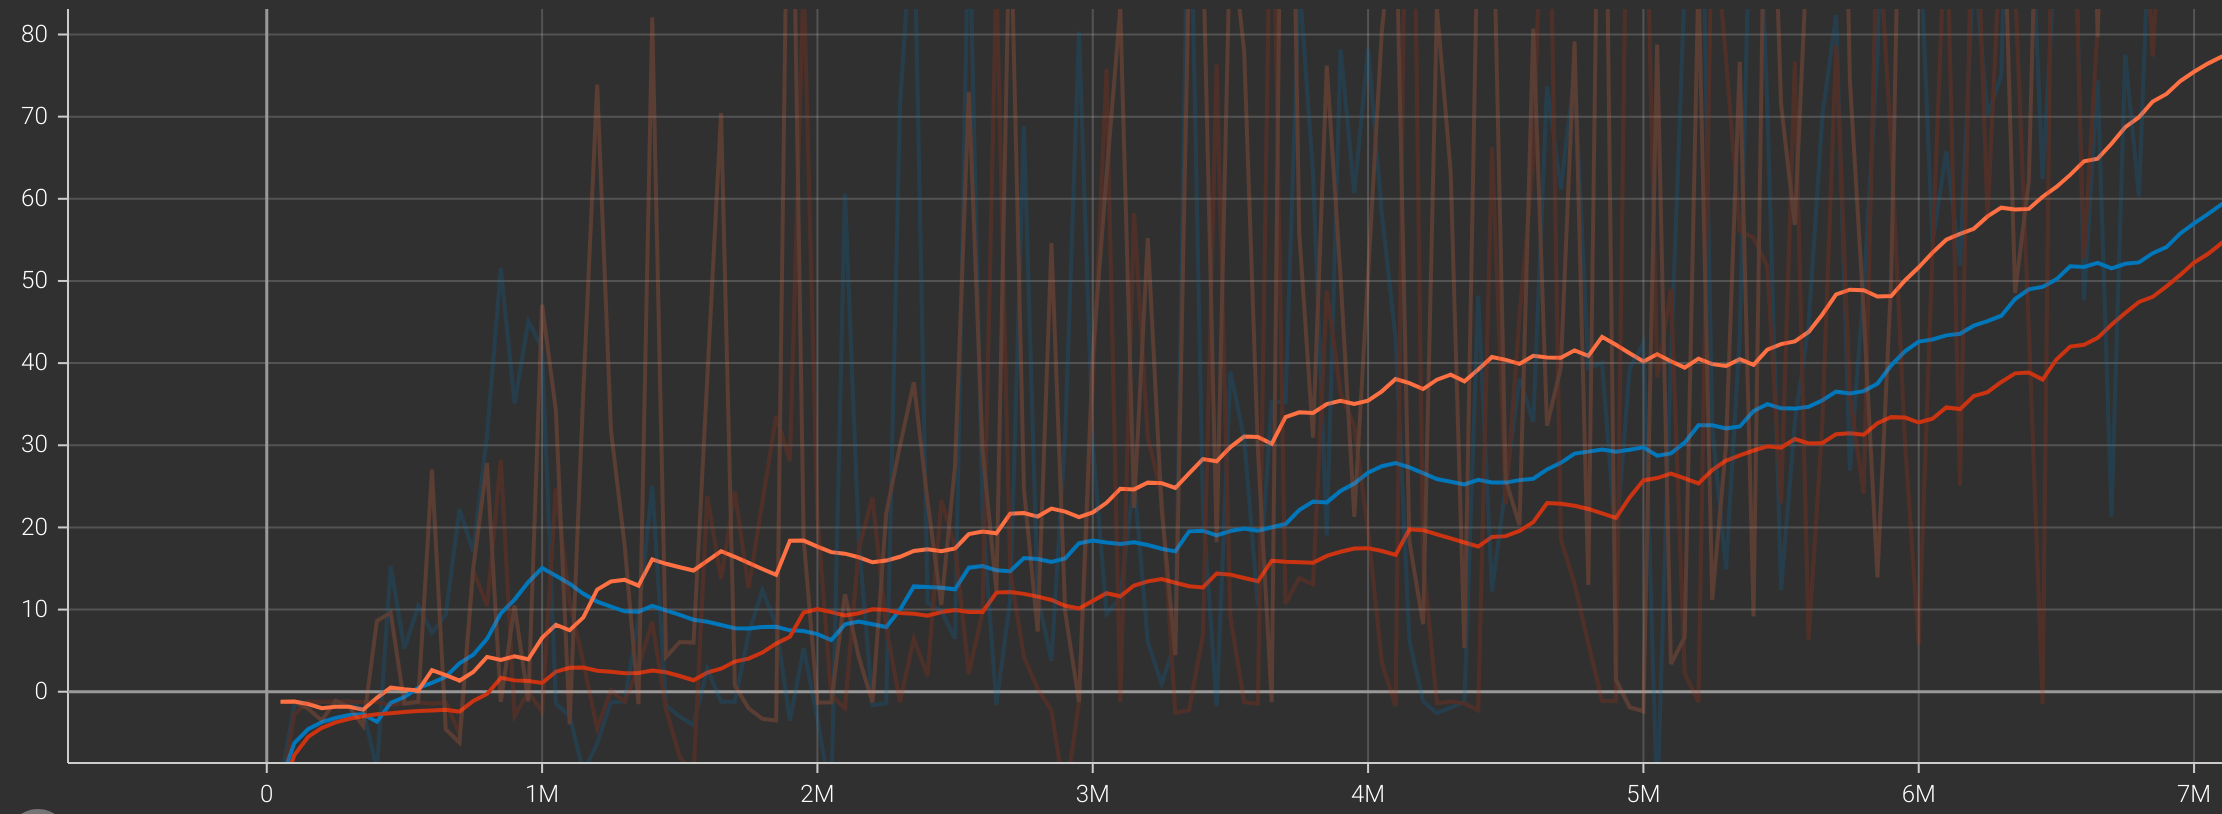
\includegraphics[width=0.9\textwidth]{images/graphs/AAT2-TL-TwoKink-AWS.png}
  \caption{\textit{Orange}: Adversarially Trained(Action Attack)
    Transfer Learned model, \textit{Blue}: Transfer Learned model,
    \textit{Red}: Baseline model. X-axis: Time steps. Y-axis:
    Cumulative Reward }
  \label{fig:my_label}
\end{figure}

\begin{itemize}
\item The AT-TL model achieves a score of 69.6 and the AAT-TL model
  achieves a score of 75.5 at the end of 7 million steps.
\item The AT-TL model gives an improvement of 21.9\% over the TL model
  and similarly the AAT-TL model gives an improvement of 32.2\%.
\item Given the stark differences in complexity of the Two-Kink Track
  and the AWS Track, this improvement in performance is a significant
  improvement over the results seen when performing vanilla transfer
  learning.
\end{itemize}

% \begin{table}[H]
% \begin{tabular}{|l|l|l|}
% \hline
% \textbf{Model}                      & \textbf{Steps (in millions)} & \textbf{Average Reward} \\ \hline
% TL Model OneKink - TwoKink & 8                   & 39.7           \\ \hline
% TL - AT OneKink - TwoKink  & 8                   & 69.8           \\ \hline
% TL - AAT OneKink - TwoKink & 8                   & 63.9           \\ \hline
% TL Model TwoKink - AWS     & 7                   & 57.1               \\ \hline
% TL - AT TwoKink - AWS      & 7                   & 69.6             \\ \hline
% TL - AAT TwoKink - AWS     & 7                   & 75.5             \\ \hline
% \end{tabular}
% \end{table}

Table \ref{tab:phase2} shows the consolidated results obtained across
Phase 2 and Phase 3 of our experimentation.
\begin{table}[H]
\begin{tabular}{|p{1.8cm}|p{1.8cm}|l|p{1.8cm}|l|p{3.2cm}|}
\hline
\textbf{Source Track} & \textbf{Target Track} & \textbf{Training Type} & \textbf{Steps ($\times 10^{6}$)} & \textbf{Average Reward} & \textbf{\%improvement (wrt TL)} \\ \hline
\multirow{3}{*}{OneKink}               & \multirow{3}{*}{TwoKink}               & TL                                      & 7                                             & 36.3                                     & -                      \\ \cline{3-6} 
                                      &                                        & AT - TL                                 & 7                                             & 65.3                                     & 79.9                   \\ \cline{3-6} 
                                      &                                        & AAT - TL                                & 7                                             & 65.5                                     & 80.4                   \\ \hline
\multirow{3}{*}{TwoKink}               & \multirow{3}{*}{AWS}                   & TL                                      & 7                                             & 57.1                                     & -                      \\ \cline{3-6} 
                                      &                                        & AT - TL                                 & 7                                             & 69.6                                     & 21.9                   \\ \cline{3-6} 
                                      &                                        & AAT - TL                                & 7                                             & 75.5                                     & 32.2                   \\ \hline
\end{tabular}
\caption{Average reward  of different Adversarial Attacks and Transfer Learned Models \\ AT - Observation Attack \\ AAT - Action Attack}
\label{tab:phase2}
\end{table}


% \begin{table}[H]
% \centering\begin{tabular}{|l|l|l|c|p{2.5cm}|}
% \hline
% \textbf{Source Track}             & \textbf{Target Track}             & \textbf{Training Type} & \textbf{Steps (in millions)} & \textbf{Average Reward} \\ \hline
% \multirow{3}{*}{OneKink} & \multirow{3}{*}{TwoKink} & TL            & 7                   & 36.3           \\ \cline{3-5} 
%                          &                          & AT - TL       & 7                   & 65.3            \\ \cline{3-5} 
%                          &                          & AAT - TL      & 7                   & 65.5           \\ \hline
% \multirow{3}{*}{TwoKink} & \multirow{3}{*}{AWS}     & TL            & 7                   &  57.1               \\ \cline{3-5} 
%                          &                          & AT - TL       & 7                   &      69.6         \\ \cline{3-5} 
%                          &                          & AAT - TL      & 7                   &       75.5         \\ \hline
% \end{tabular}
% \caption{Average reward  of different Adversarial Attacks and Transfer Learned Models \\ AT - Observation Attack \\ AAT - Action Attack}
% \label{tab:phase2}
% \end{table}
% Chapter 7

\chapter{CONCLUSION AND FUTURE WORK}

Reinforcement Learning has become a field that has found practical
applications in numerous avenues and has been adopted to solve a wide
range of industry problems. In our project, we investigated the
effectiveness of adversarial training in improving the results of
transfer learning in reinforcement learning, and conducted experiments
for the same purpose.

We conducted our experiments on 5 different tracks, namely, Oval
Track, One-Kink Track, Two-Kink Track, Barcelona Track and AWS
Track. Out of these 5 tracks, we use the One-Kink, Two-Kink and AWS
Track for transfer learning and adversarial training.

In the first phase of our project, we conducted baseline training
experiments to quantify our performance when training on a single
track from scratch. This experiment was performed on all 5 tracks.

In the second phase of our project, we trained models for a moderate
amount of time (around 1 to 2 million time steps) on a simple track,
and then transferred the trained model to a more complex track. After
transferring the model, we continued training on the new track for
about 8 million time steps. When compared with the baseline trained
from scratch, the transfer learnt models were able to achieve 5\% to
7\% better performance when given the same amount of training time.

In the third phase of our project, we introduced adversarial training
into our regimen in two different methods. In the first method, we
performed a random noise attack in order to perturb the sensory inputs
of the agent. In the second method, we added an action adversary to
the agent which picks random actions during the training process to
disturb the inputs to the agent. Both of these methods perform
significantly better than vanilla transfer learning by approximately
least 60\%.

With these results, we have shown that adversarial training
significantly improves the effectiveness of transfer learning in
reinforcement learning, and helps the agents generate better
representations of their states. We plan to examine the effectiveness
of other adversarial attacks in the future such as gradient-based
attacks.

\end{spacing}
\newpage
\appendix
% Appendix
\chapter{USING OUR CUSTOM ENVIRONMENT FOR RL EXPERIMENTATION}
% \setstretch{1.0}
% \inputminted[linenos,tabsize=2,breaklines]{csharp}{clean_code_fucnt.cs}

In this chapter we discuss how to set up Unity and the resources required for the running project. Unity is a free for personal use game development engine, and it UnityHub can be downloaded from  \href{https://store.unity.com/\#plans-individual}{https://store.unity.com/\#plans-individual}. After installing UnityHub, install Unity version 2019.4.25f1.

Clone the project repository into the system from \href{https://github.com/MaheshBharadwaj/UnityRacer}{https://github.com/MaheshBharadwaj/UnityRacer}.
Open the cloned project in UnityHub using the installed version of Unity. Click on Window $\rightarrow$ Package Manager $\rightarrow$ Unity Registry, search for MLagents version 2.1.0 and install. Finally, install the MLAgents python package using pip or conda from \href{https://pypi.org/project/mlagents/}{https://pypi.org/project/mlagents/}.

Once you have completed these steps, you will be able to explore the environments we have created. You will also be able to access the prefabs created by us in Assets $\rightarrow$ Prefabs. The 3 prefabs as seen in figure \ref{fig:prefabs} are the building blocks of all the tracks that we have created. 

Click on File $\rightarrow$ New Scene and use the track prefabs shown in \ref{fig:prefabs} to create a new track. Ensure the track is created withing a game object and drag and drop the TrackCheckpoints.cs script onto the game object. After creating the layout of the track, drag and drop the checkpoint prefab onto the track. Copy and paste the checkpoints one after another across the track. Ensure that the checkpoints are in sequential order and are roughly equidistant from each other to ensure optimal performance. We also recommend increasing the density of the number of checkpoints during sharp turns to improve the agent performance.
 
\begin{figure}[H]
    \centering
    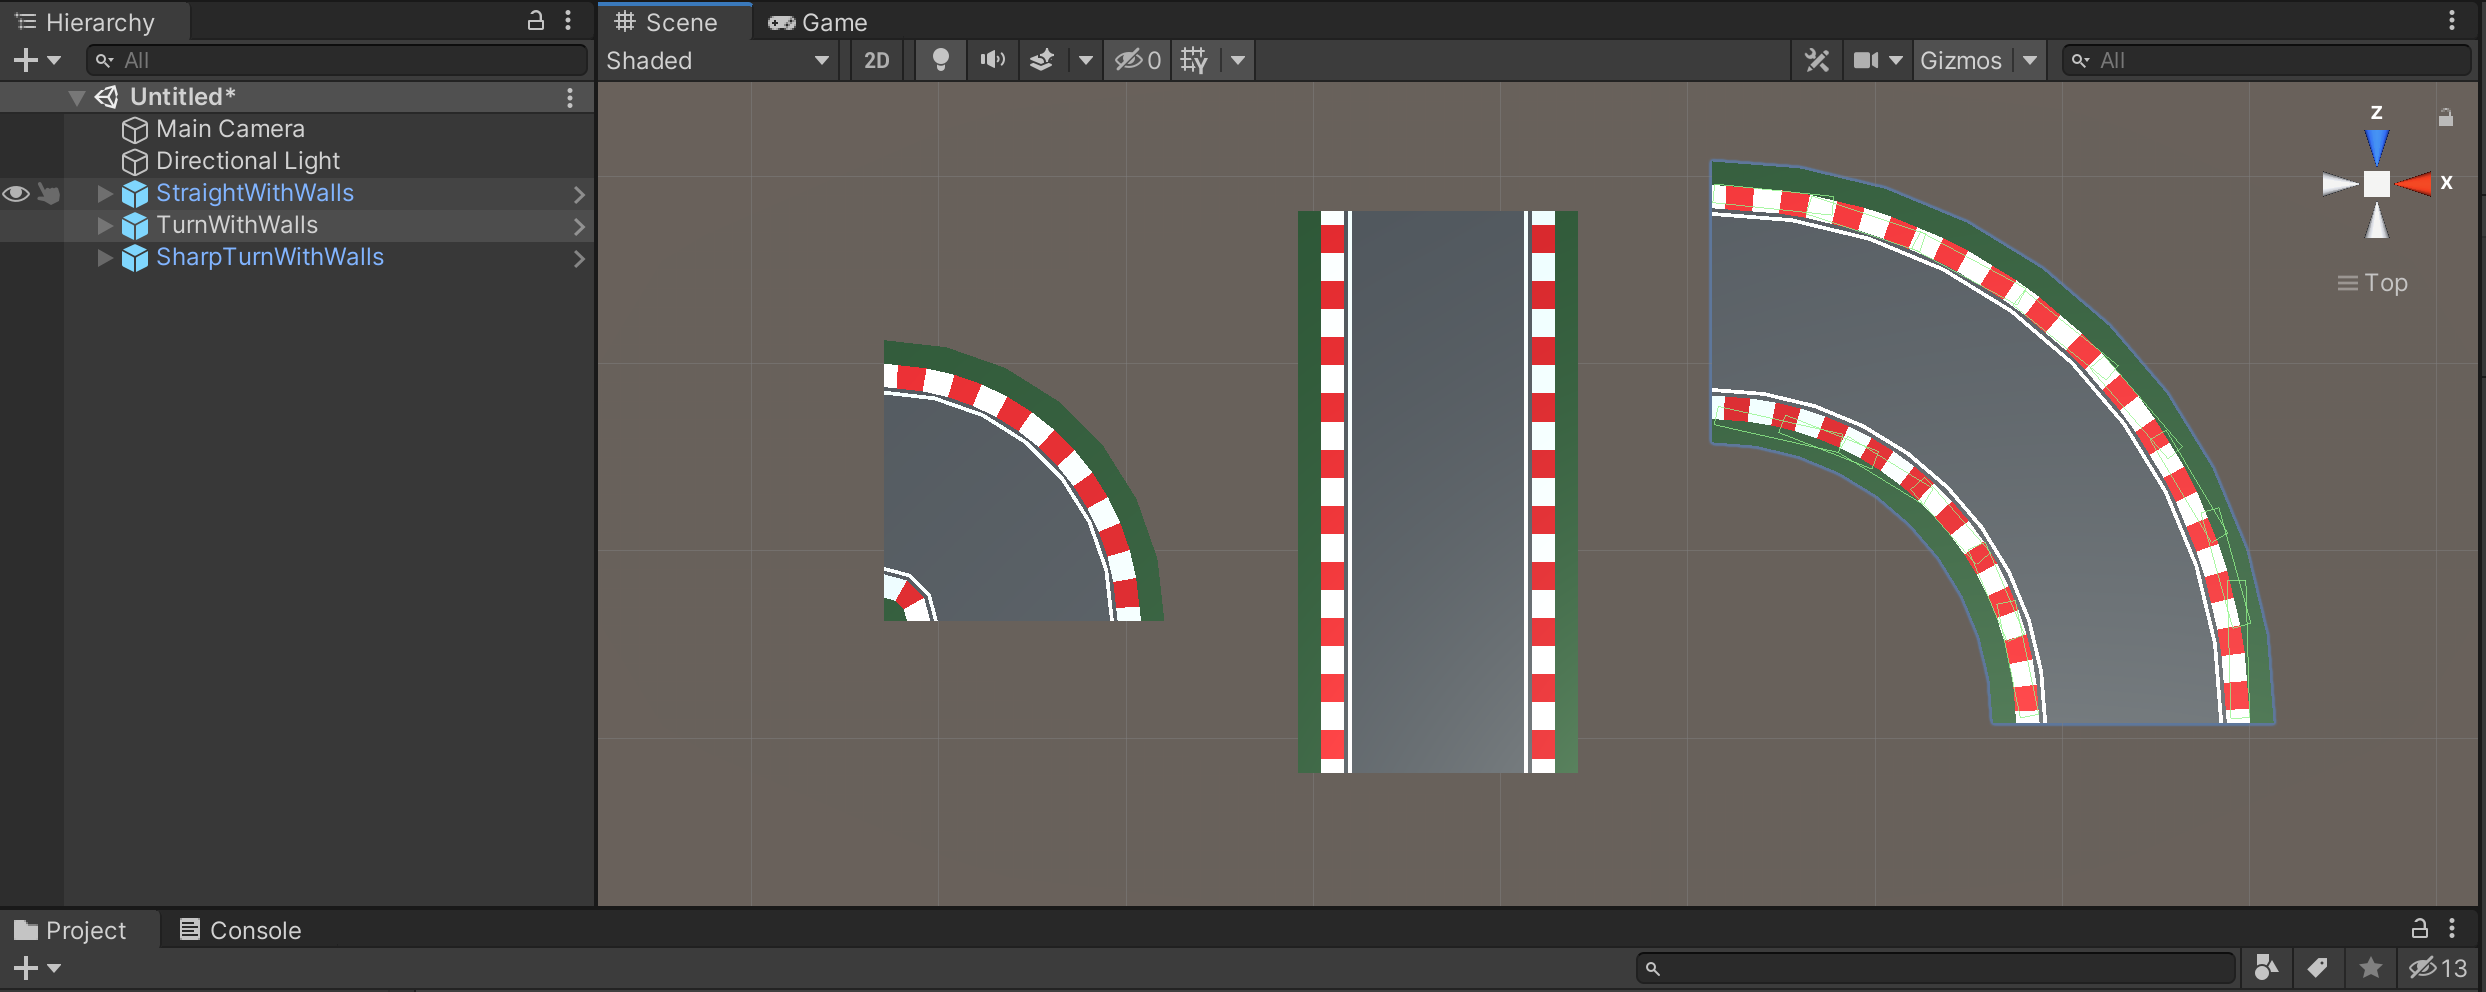
\includegraphics[width=1.0\textwidth]{images/Appendix_scene_prefabs.png}
    \caption{Prefabs L-R: Sharp Turn, Straight, Sweeping Turn}
    \label{fig:prefabs}
\end{figure}

Once the checkpoints are placed, you can drag and drop the `player' from the prefabs folder onto the track right before the first checkpoint. Adjust the position of the player appropriately. The player prefab, comes with numerous features associated with it, on clicking the player component in Unity, check the inspector panel on the right side of the console to setup the agent features.

There are two types of adversarial training. To enable the observation adversary, click on the game object in which the track is present. This will open the inspector panel on the right. In this panel check the `Is Adversarial Training' box, as seen in \ref{fig:AT-Console}
To enable action adversary, click on the player, and in the inspector panel, in the `Car Driver AI' section, set the `Action Adversary' value as a number between 0 and 1.
Shown in \ref{fig:AAT-Console}

\begin{figure}[H]
    \centering
    \begin{minipage}[b]{0.45\textwidth}
    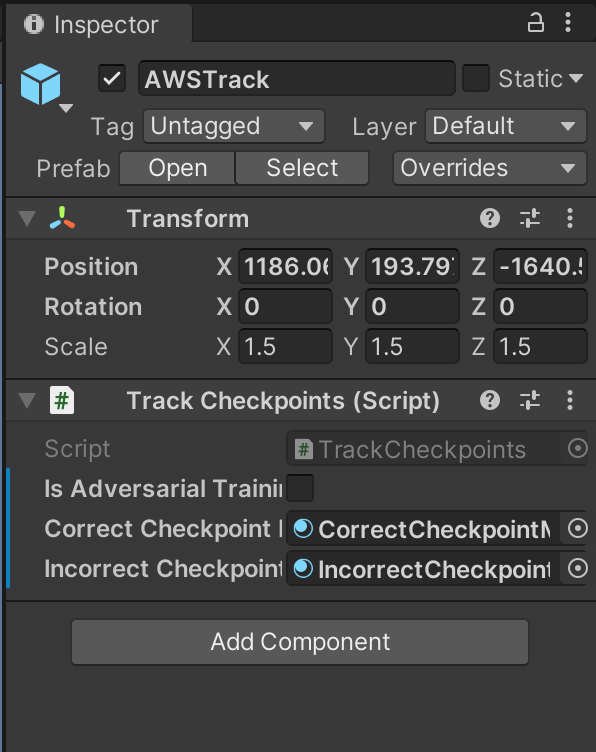
\includegraphics[width=\textwidth]{images/AT-console.png}
    \caption{Enabling AT}
    \label{fig:AT-Console}
  \end{minipage}
  \hfill
  \begin{minipage}[b]{0.45\textwidth}
    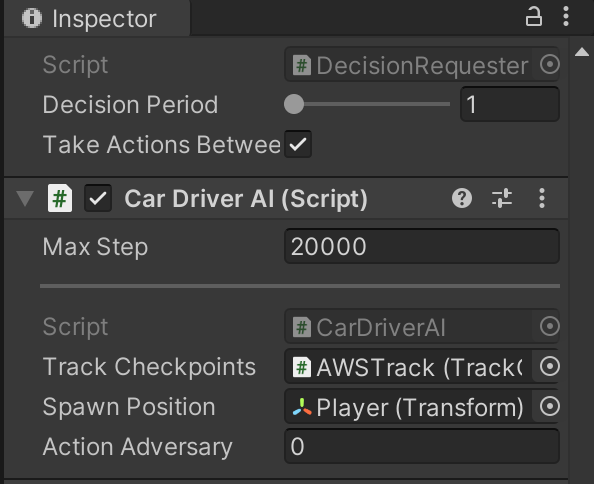
\includegraphics[width=\textwidth]{images/AAT-console.png}
    \caption{Enabling AAT}
    \label{fig:AAT-Console}
  \end{minipage}
\end{figure}


Before training, open the config file named common\_config\_ppo.yaml and set the required parameters in the file. After setting the hyperparameters, use the `mlagents-learn' command while specifying the config file and the run-id in a terminal to start the training process. After running the commamnd open the Unity environment and click on the `Play' button. Once training is finished, the model will be available as a .onnx file in the results folder within a folder having the same name as the run-id.

To use transfer learning open the config file named TL\_config.yaml and set the hyperparameters. Make sure to set the initialize\_from field with the run-id of the source task to enable transfer learning. After setting up the config file. Use the same command `mlagents learn' and specify the TL\_config file to start training process.

To test the models, click on the player component and navigate to the Behaviour parameters in the inspect panel of the console. There you can select a .onnx file model. On doing so, the player will use this model file to travel around the track.

To analyze the results go to the project folder and run the command `tensorboard --logdir results --port 6006'. After running the command open http://localhost:6006/ in a browser. This will allow you to visualize the results of the various models you have trained, on your browser. 



% \begin{itemize}
%     \item Install unity
%     \item Install ML Agents
%     \item Clone the repo for Racerdeep
%     \item Open the prefabs made for sharp turn, turn and straight
%     \item Creating a new track in a new scene
%     \item Adding behaviour parameters and setting up the scripts for the agent training.
%     \item using adversarial training.
%     \item How to config the PPO algorithim and start training
%     \item How to analyse the results
% \end{itemize}


%\addtotoc{REFERENCES}
%\input{References} 

% WORKING REF -DONT DELETE - MAHESH
\bibliographystyle{apalike}
\bibliography{ref}

% TEST REF
% \printbibliography

\end{document}
`
